\chapter{A Numerical Evaluation of the PEM} \label{ch:results}
%
This chapter provides a detailed numerical assessment of several partitioned element methods, with specific emphasis placed upon the DG-PEM. A numerical measure of polynomial reproducibility is introduced and utilized to investigate the level of interpolation error incurred by different formulations of the PEM. Linear and quadratic finite element patch tests are conducted in both 2- and 3-dimensions, with comparisons drawn between the FEM and the PEM. The behavior of irregularly-shaped polygonal elements is investigated, and the effects of short element edges within 2-dimensional Voronoi meshes are examined further. Convergence studies are carried out to compare the accuracy of the PEM with that of the FEM. The chapter concludes with a number of demonstrative problems, illustrating the ability of the PEM to accommodate finite deformations and elasto-plastic material behavior.

\section{Tests for Polynomial Reproducibility}

Herein, an investigation is conducted to assess the degree to which polynomial reproducibility is achieved by a given partitioned element methodology. Reproducibility is assessed by an \textit{interpolation error} metric, defined in the following section.

\subsection*{Interpolation Error}

Consider an arbitrary polytopal element $\Omega \subset \mathbb{R}^d$. Let $u \in P^k (\Omega)$ denote a scalar polynomial field of maximal degree $k$, written in terms of the monomials:
\begin{equation}
        u (\mathbf{X}) = \sum_{|\alpha| \leq k} c_{\alpha} \, \mathbf{X}^{\alpha}.
\end{equation}
The $H^1(\Omega)$ norm of any scalar field $u \in H^1(\Omega)$ is denoted
\begin{equation}
        ||u||_{H^1} = \left[ \langle u, \, u \rangle_{H^1} \right]^{1/2},
\end{equation}
where
\begin{equation}
       \langle u,v \rangle_{H^1} = \int_{\Omega} (u \, v + u_{,i} v_{,i}) \, d\Omega
\end{equation}
is the $H^1(\Omega)$ inner product of $u, \,v \in H^1(\Omega)$. Denote $u^h$ as the approximate representation of $u$ over $\Omega$ using the element's shape functions $\left\{ \varphi_A \right\}_{A=1}^{N^\Omega_V}$:
\begin{equation}
        u^h (\mathbf{X}) = \sum_{A = 1}^{N^{\Omega}_V} \varphi_A (\mathbf{X}) \, u(\mathbf{X}_A).
\end{equation}

Recall that the space of all polynomials of maximal degree $k$ is denoted $P^k (\Omega)$. The sub-space $\bar{P}^k (\Omega) \subset P^k (\Omega)$ contains only those polynomials with unit $H^1 (\Omega)$ norm:
\begin{equation}
        \bar{P}^k (\Omega) = \{ u : u \in P^k (\Omega), ||u||_{H^1} = 1 \}.
\end{equation}

The \textit{interpolation error} $E_k (\Omega)$ on the element $\Omega$ over the polynomials of maximal degree $k$ is defined as
\begin{equation}
        E_k (\Omega) \equiv \sup_{u \in \bar{P}^k (\Omega)} || u(\mathbf{X}) - u^h(\mathbf{X}) ||_{H^1} = \sup_{u \in P^k (\Omega)} \frac{|| u(\mathbf{X}) - u^h(\mathbf{X}) ||_{H^1}}{|| u(\mathbf{X}) ||_{H^1}}.
\end{equation}
In the numerical computation of this error measure, the polynomial coefficients $c_\alpha$ of $u \in \bar{P}^k (\Omega)$ which yield the maximal error must be determined. Denote $e_\alpha$ as the error in the approximation of the monomial $\mathbf{X}^\alpha$:
\begin{equation}
        e_\alpha = \mathbf{X}^{\alpha} - \sum_{A = 1}^{N^{\Omega}_V} \varphi_A (\mathbf{X}) \, \mathbf{X}_A^{\alpha}.
\end{equation}
Consequently,
\begin{equation}
        \left[ E_k (\Omega) \right]^2 = \max_{c_\gamma} \sum_{|\alpha| \leq k} \sum_{|\beta| \leq k} c_{\alpha} c_{\beta} \langle e_\alpha, e_\beta \rangle_{H^1},
\end{equation}
subject to the constraint
\begin{equation}
        g(c_\gamma) = 1 - \sum_{|\alpha| \leq k} \sum_{|\beta| \leq k} c_{\alpha} c_{\beta} \langle \mathbf{X}^\alpha, \mathbf{X}^\beta \rangle_{H^1} = 0.
\end{equation}
Using the method of Lagrange multipliers, we may rewrite the above constrained optimization problem as
\begin{equation}
        \left[ E_k (\Omega) \right]^2 = \max_{c_\gamma, \lambda} \Lambda (c_\gamma,\lambda),
\end{equation}
where $\Lambda (c_\gamma,\lambda)$ is the Lagrangian:
\begin{equation}
        \Lambda (c_\gamma, \lambda) = \max_{c_\gamma} \sum_{|\alpha| \leq  k} \sum_{|\beta| \leq k} c_{\alpha} c_{\beta} \langle e_\alpha, e_\beta \rangle_{H^1} + \lambda g(c_\gamma).
\end{equation}
Observe that
\begin{equation}
        \frac{\partial}{\partial \lambda} \Lambda (c_\gamma, \lambda) = g(c_\gamma) = 0,
\end{equation}
and
\begin{equation}
        \frac{\partial}{\partial c_\gamma} \Lambda (c_\gamma, \lambda) = \sum_{|\alpha| \leq k} \sum_{|\beta| \leq k} \frac{\partial}{\partial c_\gamma} (c_{\alpha} c_{\beta}) \langle e_\alpha, e_\beta \rangle_{H^1} + \lambda \frac{\partial}{\partial c_\gamma} g(c_\gamma) = 0.
\end{equation}
This yields
\begin{equation}
        \sum_{|\alpha| \leq k} c_{\alpha} \left[ \langle e_\alpha, e_\gamma \rangle_{H^1} - \lambda \langle \mathbf{X}^\alpha, \mathbf{X}^\gamma \rangle_{H^1} \right] = 0 \quad \forall |\gamma| \leq k,
\end{equation}
or, in matrix-vector notation:
\begin{equation}
        (\mathbf{A} - \lambda \mathbf{B}) \mathbf{c} = \mathbf{0},
\end{equation}
corresponding to the generalized eigenvalue problem, where
\begin{equation}
        A_{\alpha \beta} = \langle e_\alpha, e_\beta \rangle_{H^1}, \qquad B_{\alpha \beta} = \langle \mathbf{X}^\alpha, \mathbf{X}^\beta \rangle_{H^1},
\end{equation}
are both real, symmetric matrices. Since $\mathbf{B}$ is positive-definite, we determine that it is invertible, and therefore we may solve the equivalent eigenvalue problem:
\begin{equation}
        (\mathbf{B}^{-1} \mathbf{A} - \lambda \mathbf{1}) \mathbf{c} = \mathbf{0}.
\end{equation}
The square root of the maximum eigenvalue $\lambda_{\max}$ of $\mathbf{B}^{-1} \mathbf{A}$ yields the interpolation error $E_k (\Omega) = \sqrt{\lambda_{\max}}$. This can be seen more directly if we view $\left[ E_k (\Omega) \right]^2$ to be the generalized Rayleigh quotient of $\mathbf{A}$ and $\mathbf{B}$:
\begin{equation}
        E_k (\Omega) = \max_{\mathbf{c}} \sqrt{\frac{\mathbf{c}^T \mathbf{A} \mathbf{c}}{\mathbf{c}^T \mathbf{B} \mathbf{c}}} = \sqrt{\lambda_{\max}}.
\end{equation}
For simplicity in the numerical computation of $E_k (\Omega)$, we assume that the entries of $\mathbf{A}$ and $\mathbf{B}$ will be computed approximately using the element's quadrature rules, i.e.
\begin{equation}
        \langle e_\alpha, e_\beta \rangle_{H^1} \approx \sum_{q=1}^{N^{\Omega}_{qp}} w_q (e_{\alpha}^{q} e_{\beta}^{q} + e_{\alpha,i}^{q} e_{\beta,i}^{q}),
\end{equation}
\begin{equation}
        \langle \mathbf{X}^\alpha, \mathbf{X}^\beta \rangle_{H^1} \approx \sum_{q=1}^{N^{\Omega}_{qp}} w_q (\mathbf{X}^{\alpha}_{q} \mathbf{X}^{\beta}_{q} + \mathbf{X}^{\alpha}_{q,i} \mathbf{X}^{\beta}_{q,i}),
\end{equation}
where
\begin{equation}
        e_{\alpha}^{q} = \mathbf{X}^{\alpha}_{q} - \sum_{A = 1}^{N^{\Omega}_V} \varphi_A (\mathbf{X}_{q}) \, \mathbf{X}_A^{\alpha}, \qquad e_{\alpha,i}^{q} = \mathbf{X}^{\alpha}_{q,i} - \sum_{A = 1}^{N^{\Omega}_V} \varphi_{A,i} (\mathbf{X}_{q}) \, \mathbf{X}_A^{\alpha}.
\end{equation}

If a given element is capable of reproducing all polynomials up to degree $k$, then clearly $E_k(\Omega) = 0$. This property is used to verify that the shape function approximations obtained via a particular formulation of the PEM satisfy the requirements of polynomial reproducibility.

\subsection*{Verification of Polynomial Reproducibility for PEM Elements}

Through a series of numerical experiments, it is confirmed that both the CG-PEM and the DG-PEM satisfy the requirements of polynomial reproducibility. Particular attention is paid to low-order PEM elements (i.e. $k=1$), where satisfaction of the condition $E_1 (\Omega) = 0$ is sufficient to demonstrate reproducibility for a given element $\Omega$.

Consider the arbitrary polygonal element and its corresponding edge-based partition illustrated in Figure \ref{fig:reproducing_element_shape}. The harmonic shape functions defined on this partitioned element were approximated using the CG-PEM and the DG-PEM. Unless otherwise noted, the NIPG version of the DG-PEM ($\epsilon = +1$) was utilized throughout.

\begin{figure}[!h]
  \centering
  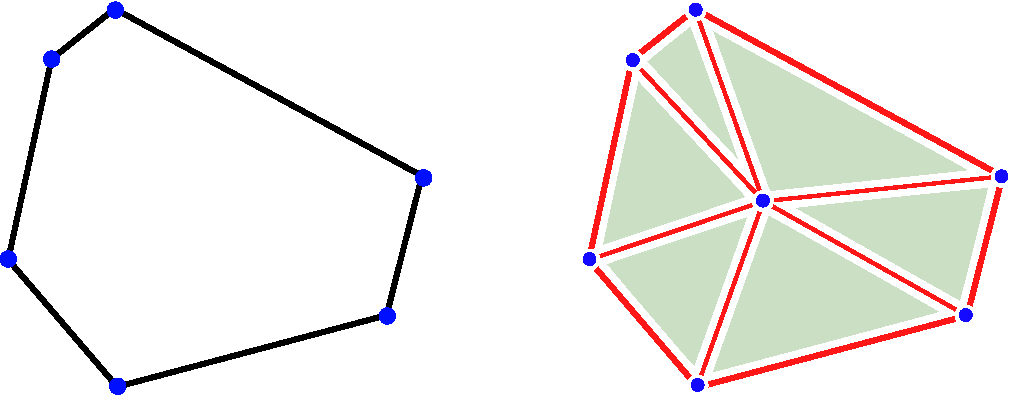
\includegraphics[width=3.5in]{figures/reproducing_element_shape.pdf}  \caption{A representative polygonal element and its corresponding edge-based partition.}
  \label{fig:reproducing_element_shape}
\end{figure}

For the partitioned element under consideration, the interpolation error of order $k=1$ for the CG-PEM was computed as $E_1 (\Omega) = 2.5465 \times 10^{-16}$ (on the order of machine precision). For the DG-PEM, the interpolation error was observed to be dependent upon the accuracy of the computations performed in solving the linear system of equations in (\ref{eq:dgpem_linear_system}). The log of $\kappa(\mathbf{J})$ provides a useful indicator of the number of digits of precision lost in computing $\mathbf{J}^{-1}$. This loss of precision is reflected by a corresponding increase in the interpolation error measure. Table \ref{tab:interpolation_error_and_condJ_k1} illustrates the connection between $E_1 (\Omega)$ and $\kappa(\mathbf{J})$ for various DG-PEM penalty parameter values. 

\begin{table}
\centering
\begin{subtable}{1.0\textwidth}
\centering
\begin{tabular}{| c || c | c | c | c |}
    \hline
$E_1 (\Omega)$ & $\alpha_{\gamma0} = 10^{-3}$ & $\alpha_{\gamma0} = 10^{0}$ & $\alpha_{\gamma0} = 10^{3}$ & $\alpha_{\gamma0} = 10^{6}$ \\ \hline \hline
$\alpha_{\gamma1} = 0.0$	& 1.66E-013 & 7.48E-016 & 4.70E-014 & 1.79E-010 \\ \hline
$\alpha_{\gamma1} = 10^{0}$ & 1.65E-013 & 9.67E-016 & 8.73E-015 & 2.51E-011 \\ \hline
$\alpha_{\gamma1} = 10^{3}$ & 1.01E-012 & 2.66E-013 & 1.36E-015 & 4.49E-014 \\ \hline
$\alpha_{\gamma1} = 10^{6}$ & 1.13E-009 & 3.13E-010 & 7.10E-013 & 9.03E-016 \\
    \hline
    \end{tabular}
    \caption{Interpolation error: $E_1 (\Omega)$}
    \label{tab:interpolation_error_k1}
\end{subtable}% <---- don't forget this %
\\
\begin{subtable}{1.0\textwidth}
\centering
\begin{tabular}{| c || c | c | c | c |}
    \hline
$\kappa(\mathbf{J})$ & $\alpha_{\gamma0} = 10^{-3}$	&	$\alpha_{\gamma0} = 10^{0}$	&	$\alpha_{\gamma0} = 10^{3}$	&	$\alpha_{\gamma0} = 10^{6}$ \\ \hline \hline
$\alpha_{\gamma1} = 0.0$	&	5.44E+002 & 4.07E+000 & 5.94E+003 & 5.96E+006 \\ \hline
$\alpha_{\gamma1} = 10^{0}$	&	4.96E+003 & 2.01E+001 & 9.33E+002 & 9.29E+005 \\ \hline
$\alpha_{\gamma1} = 10^{3}$	&	1.58E+007 & 2.50E+004 & 6.96E+001 & 1.11E+003 \\ \hline
$\alpha_{\gamma1} = 10^{6}$	&	2.37E+010 & 2.50E+007 & 6.86E+004 & 6.98E+001 \\
    \hline
    \end{tabular}
    \caption{DG-PEM linear system conditioning: $\kappa(\mathbf{J})$}
    \label{tab:condJ_k1}
\end{subtable}

\caption{Computed values of $E_1 (\Omega)$ and $\kappa(\mathbf{J})$ for the element in Figure \ref{fig:reproducing_element_shape}, using various DG-PEM penalty parameter settings.}
\label{tab:interpolation_error_and_condJ_k1}
\end{table}

The results in table \ref{tab:interpolation_error_and_condJ_k1} confirm that $\mathbf{J}$ will become poorly conditioned if either of the two penalty parameters $\alpha_{\gamma0}$ or $\alpha_{\gamma1}$ are sufficiently large. This is true regardless of how the DG polynomial bases are specified for each geometric entity. Under certain circumstances, $\mathbf{J}$ will remain well-conditioned if both $\alpha_{\gamma0}$ and $\alpha_{\gamma1}$ are kept roughly proportional to one another, for all values of $\alpha_{\gamma0}, \, \alpha_{\gamma1} > 0$. If $\alpha_{\gamma0}$ and $\alpha_{\gamma1}$ are increased proportionally to one another, one recovers the behavior of the pure penalty DG-PEM in (\ref{eq:pure_penalty}).

Other factors which impact the condition number of $\mathbf{J}$ (such as element shape) may therefore lead to increased interpolation errors. Specifically, consider the case where the element in Figure \ref{fig:reproducing_element_shape} is scaled anisotropically by a factor of $0.01$ in the vertical direction, yielding a comparatively thin element with an aspect ratio of 100:1. For this element, the interpolation error using the CG-PEM increases only slightly, to $E_1 (\Omega) = 6.9817 \times 10^{-15}$. The corresponding values of $E_1 (\Omega)$ and $\kappa(\mathbf{J})$ for the DG-PEM are presented in table \ref{tab:thin_interpolation_error_and_condJ_k1}.

\begin{table}
\centering
\begin{subtable}{1.0\textwidth}
\centering
\begin{tabular}{| c || c | c | c | c |}
    \hline
$E_1 (\Omega)$ & $\alpha_{\gamma0} = 10^{-3}$ & $\alpha_{\gamma0} = 10^{0}$ & $\alpha_{\gamma0} = 10^{3}$ & $\alpha_{\gamma0} = 10^{6}$ \\ \hline \hline
$\alpha_{\gamma1} = 0.0$	& 3.02E-014 & 9.01E-015 & 5.22E-013 & 1.59E-009 \\ \hline
$\alpha_{\gamma1} = 10^{0}$ & 3.99E-014 & 1.37E-014 & 2.02E-013 & 3.12E-012 \\ \hline
$\alpha_{\gamma1} = 10^{3}$ & 2.44E-011 & 6.48E-012 & 1.89E-012 & 3.34E-013 \\ \hline
$\alpha_{\gamma1} = 10^{6}$ & 1.52E-007 & 4.97E-008 & 1.85E-009 & 3.69E-012 \\
    \hline
    \end{tabular}
    \caption{Interpolation error: $E_1 (\Omega)$}
    \label{tab:thin_interpolation_error_k1}
\end{subtable}% <---- don't forget this %
\\
\begin{subtable}{1.0\textwidth}
\centering
\begin{tabular}{| c || c | c | c | c |}
    \hline
$\kappa(\mathbf{J})$ & $\alpha_{\gamma0} = 10^{-3}$	&	$\alpha_{\gamma0} = 10^{0}$	&	$\alpha_{\gamma0} = 10^{3}$	&	$\alpha_{\gamma0} = 10^{6}$ \\ \hline \hline
$\alpha_{\gamma1} = 0.0$	& 9.07E+003 & 1.39E+002 & 1.14E+005 & 1.33E+008 \\ \hline
$\alpha_{\gamma1} = 10^{0}$	& 3.52E+005 & 1.75E+003 & 1.97E+004 & 3.67E+005 \\ \hline
$\alpha_{\gamma1} = 10^{3}$	& 1.17E+009 & 2.46E+006 & 2.61E+005 & 2.32E+004 \\ \hline
$\alpha_{\gamma1} = 10^{6}$	& 1.77E+012 & 2.45E+009 & 2.52E+008 & 3.07E+005 \\
    \hline
    \end{tabular}
    \caption{DG-PEM linear system conditioning: $\kappa(\mathbf{J})$}
    \label{tab:thin_condJ_k1}
\end{subtable}

\caption{Computed values of $E_1 (\Omega)$ and $\kappa(\mathbf{J})$ for a comparatively thin element with an aspect ratio of 100:1, using various DG-PEM penalty parameter settings.}
\label{tab:thin_interpolation_error_and_condJ_k1}
\end{table}

Careful selection of $\alpha_{\gamma0}$ and $\alpha_{\gamma1}$ is warranted for the sake of minimizing the resulting interpolation error. For general applications in which an edge-based partitioning scheme is employed, it is suggested that the parameter values be chosen such that $\alpha_{\gamma0} = 10.0$ and $\alpha_{\gamma1} = 0.0$. Nonetheless, a more thorough parameter sensitivity analysis is recommended.

\section{Finite Element Patch Tests}

Several finite element patch tests for CG-PEM and DG-PEM elements are investigated. The tests are similar to the ones introduced by Irons in the Appendix of \cite{Irons:65}. Passage of such tests is argued to be a necessary and sufficient condition for convergence \cite{Simo&Taylor:86}, though this claim has been disputed, namely by Stummel in \cite{Stummel:80}. Nonetheless, patch tests are useful indicators of the expected convergence properties for conforming finite elements. Linear and quadratic patch tests in both 2- and 3-dimensions are considered.

Patch test errors were measured in terms of the normalized $L^2 (\Omega)$ error metrics for displacement and stress:
\begin{equation}
	\frac{||\mathbf{u}^h - \mathbf{u}||}{||\mathbf{u}||} = \sqrt{\frac{\int_{\mathcal{B}_0} (\mathbf{u}^h - \mathbf{u}) \cdot (\mathbf{u}^h - \mathbf{u}) \, dV}{\int_{\mathcal{B}_0} \mathbf{u} \cdot \mathbf{u} \, dV}},
\end{equation}
\begin{equation}
	\frac{||\boldsymbol{\sigma}^h - \boldsymbol{\sigma}||}{||\boldsymbol{\sigma}||} = \sqrt{\frac{\int_{\mathcal{B}_0} (\boldsymbol{\sigma}^h - \boldsymbol{\sigma}) \colon (\boldsymbol{\sigma}^h - \boldsymbol{\sigma}) \, dV}{\int_{\mathcal{B}_0} \boldsymbol{\sigma} \colon \boldsymbol{\sigma} \, dV}},
	\label{eq:normalized_stress_error}
\end{equation}
where $\mathbf{u}$ and $\boldsymbol{\sigma}$ denote the exact solutions for the displacement and stress fields, respectively.

For all of the tests considered, both the CG-PEM and DG-PEM utilized an edge-based partitioning scheme and composite mid-point quadrature rules for each element. Unless otherwise noted, the parameters for the DG-PEM were selected as $\epsilon = +1$, $\alpha_{\gamma0} = 10.0$, and $\alpha_{\gamma1} = 0.0$. Further, the DG-PEM was tested both with and without using the gradient correction scheme presented in \cite{Talischi:15}. These corrections were applied to the test function gradients alone (yielding a ``nonsymmetric correction'' scheme), or to both the trial and test function gradients (yielding a ``symmetric correction'' scheme).

\subsection*{Linear Patch Tests in 2D}

\begin{figure}[!h]
    \centering
    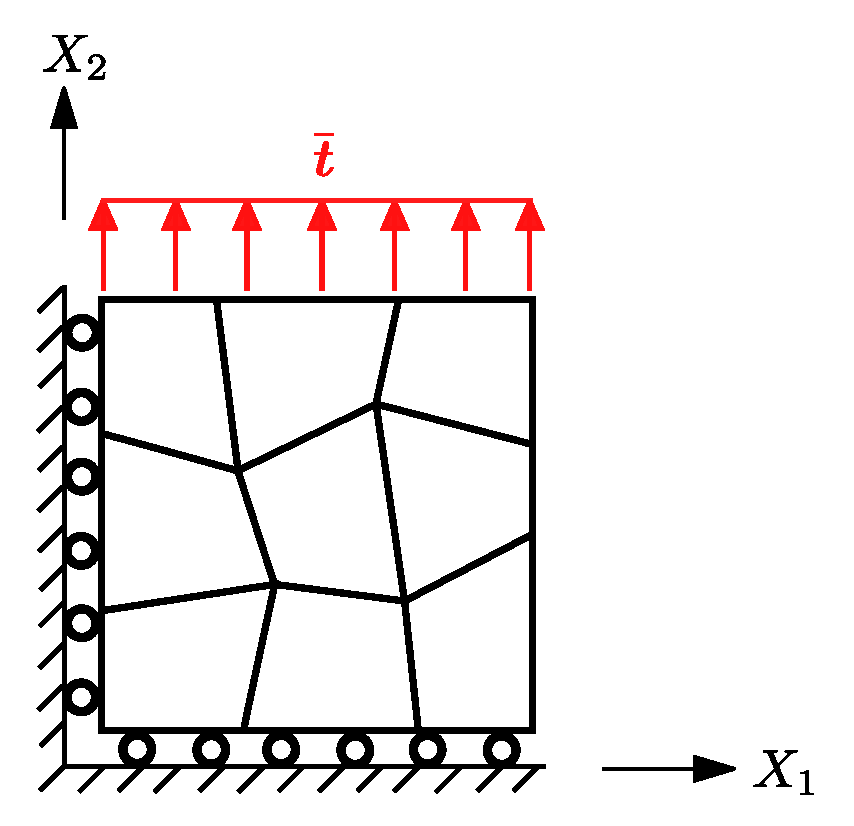
\includegraphics[width=2.5in]{figures/linear_patch_test.pdf}
    	\caption{Depiction of the 2D linear patch test.}
    \label{fig:linear_patch_test}
\end{figure}

The linear patch test consists of a square patch of elements with dimensions $L \times L$, as shown in Figure \ref{fig:linear_patch_test}. The normal components of displacement on the $-X_1$ and $-X_2$ faces of the patch are constrained such that
\begin{equation}
	u_1 (X_1 = 0) = 0, \quad u_2 (X_2 = 0) = 0.
\end{equation}
A constant vertical traction $\bar{\mathbf{t}} = (0, \, T)$ is prescribed on the $+X_2$ face of the patch. For a linear elastic body under plane strain conditions, an exact solution for the in-plane displacement and stress fields is easily obtained:
\begin{equation}
	u_1 (\mathbf{X}) = - \frac{\nu}{2 \mu} T X_1, \quad u_2 (\mathbf{X}) = \frac{(1-\nu)}{2 \mu} T X_2,
\end{equation}
\begin{equation}
	\sigma_{11} (\mathbf{X}) = \sigma_{12} (\mathbf{X}) = 0, \quad \sigma_{22} (\mathbf{X}) = T.
\end{equation}

The two meshes depicted in Figure \ref{fig:patch_test_meshes} are considered. The PEM was used on the polygonal mesh, whereas the FEM with standard 4-nodes isoparametric elements was used on the quadrilateral mesh.
\begin{figure}[!h]
    \centering
    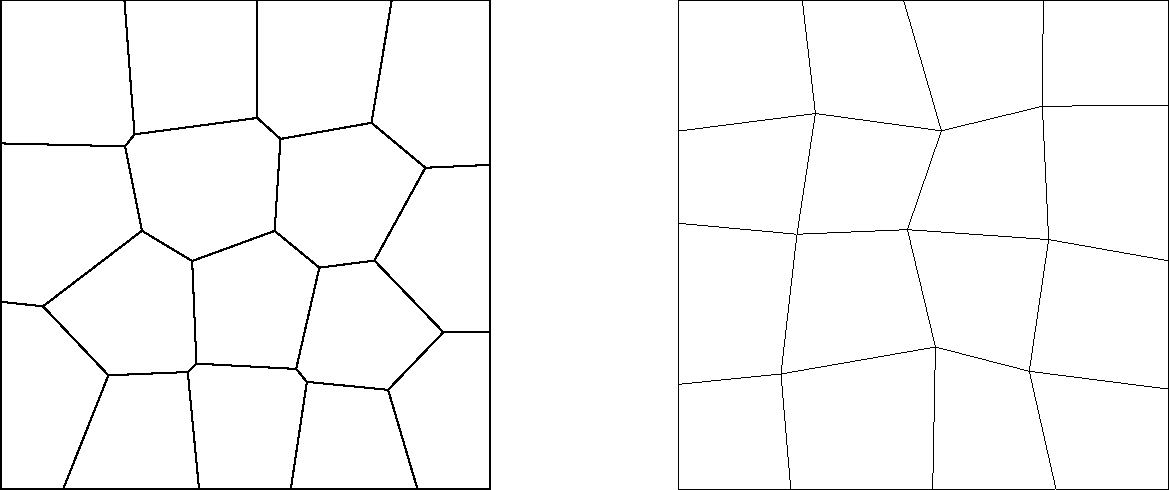
\includegraphics[width=4.0in]{figures/patch_test_meshes.pdf}
    	\caption{Meshes used for the linear patch test: (left) polygonal mesh, (right) distorted quadrilateral mesh.}
    \label{fig:patch_test_meshes}
\end{figure}

Linear patch test errors for the FEM, CG-PEM, and DG-PEM are explored. The results of these tests may be found in table \ref{tab:linear_patch_test}.

\begin{table}[!ht]
  \begin{center}
    \begin{tabular}{| l || c | c |}
    \hline
           & $||\mathbf{u}^h - \mathbf{u}|| / ||\mathbf{u}||$ & $||\boldsymbol{\sigma}^h - \boldsymbol{\sigma}|| / ||\boldsymbol{\sigma}||$ \\ \hline \hline
    FEM (4-node quadrilaterals) & 5.1568E-015 & 7.7395E-016 \\ \hline
    CG-PEM (no gradient correction) & 5.9125E-012 & 5.1637E-012 \\ \hline
    DG-PEM (no gradient correction) & 2.7721E-005 & 3.0904E-004 \\ \hline
    DG-PEM (symmetric correction) & 6.2750E-012 & 5.3521E-012 \\ \hline
    DG-PEM (nonsymmetric correction) & 6.2673E-012 & 5.3494E-012 \\
    \hline
    \end{tabular}
    \caption{Linear patch test results comparison for FEM, CG-PEM, and DG-PEM.}
    \vspace{-5pt}
    \label{tab:linear_patch_test}
    \vspace{-10pt}
  \end{center}
\end{table}

The classical FEM produces errors on the order of machine precision. The CG-PEM produces results that are only slightly less accurate. As confirmed by (\ref{eq:cg_pem_integration_consistency}), the integration errors for the CG-PEM are negligible, and the resulting patch test errors are unaffected by the use (or disuse) of a gradient correction scheme. In contrast, the DG-PEM produces noticeable errors if no gradient correction scheme is employed. Using either of the symmetric or nonsymmetric gradient correction schemes with the DG-PEM yields comparable accuracy to the CG-PEM.

These observations help to illuminate an important point regarding integration consistency. Consider the consistency equations in (\ref{eq:consistency}). It is remarked that any continuous field $\varphi_a \in C^0 (\Omega_e)$ integrated exactly in (\ref{eq:consistency}) will lead to direct satisfaction of quadrature consistency. Such is the case for linear CG-PEM elements. However, if $\varphi_a$ is not a continuous field, neither (\ref{eq:consistency}) nor quadrature consistency will be satisfied, in general. Such is the case for the DG-PEM, even if exact integration is used. The consequence is violation of patch tests. This can be mitigated through the use of a gradient correction scheme, or alternatively through an appropriate selection of the DG-PEM parameters. Specifically, in the limit as $\alpha_{\gamma0} \rightarrow \infty$, the DG-PEM reduces to the CG-PEM, and the resulting patch test errors can be eliminated. Table \ref{tab:linear_patch_test_parameter_study} demonstrates this behavior for increasing values of $\alpha_{\gamma0}$, in the absence of a gradient correction scheme.

\begin{table}[!ht]
  \begin{center}
    \begin{tabular}{| l || c | c | c | c | c |}
    \hline
    DG-PEM & $\alpha_{\gamma0} = 10^{-6}$ & $\alpha_{\gamma0} = 10^{-3}$ & $\alpha_{\gamma0} = 10^{0}$ & $\alpha_{\gamma0} = 10^{3}$ & $\alpha_{\gamma0} = 10^{6}$ \\ \hline \hline
    	$\alpha_{\gamma1} = 0.0$ & 2.8433E-009 & 2.8152E-006 & 3.3114E-004 & 4.8035E-006 & 4.8278E-009 \\ \hline
    $\alpha_{\gamma1} = 10^{-3}$ & 2.8505E-009 & 2.8224E-006 & 3.2288E-004 & 4.9805E-006 & 5.0082E-009 \\ \hline
    $\alpha_{\gamma1} = 10^{0}$ & 3.4853E-009 & 3.4604E-006 & 2.4827E-003 &  7.4284E-004 & 8.6376E-007 \\ \hline
    $\alpha_{\gamma1} = 10^{3}$ & 3.5460E-009 & 3.5450E-006 & 3.0047E-003 & 1.3898E-002 & 7.4705E-004 \\ \hline
    $\alpha_{\gamma1} = 10^{6}$ & 3.5457E-009 & 3.5456E-006 & 3.0054E-003 & 1.4604E-002 & 1.3953E-002 \\
    \hline
    \end{tabular}
    \caption{Computed values of $||\boldsymbol{\sigma}^h - \boldsymbol{\sigma}|| / ||\boldsymbol{\sigma}||$ for the DG-PEM using various penalty parameter settings. No gradient correction scheme was utilized. Identical trends were observed for $||\mathbf{u}^h - \mathbf{u}|| / ||\mathbf{u}||$.}
    \vspace{-5pt}
    \label{tab:linear_patch_test_parameter_study}
    \vspace{-10pt}
  \end{center}
\end{table}

Additionally, it is noted that the DG-PEM recovers integration consistency in the limit as $\alpha_{\gamma0} \rightarrow 0$. This is a direct consequence of (\ref{eq:weak_compatibility_enforcement}). It is tempting to want to specify $\alpha_{\gamma0}$ to be sufficiently small/large enough to reduce patch test errors to an acceptable level. However, this thinking must be tempered by an understanding of the effects of interpolation error on patch test errors. Recall that the interpolation error $E_1 (\Omega)$ for a given element is controlled largely by the conditioning of $\mathbf{J}$. In turn, $\kappa (\mathbf{J})$ will be adversely affected by sufficiently small/large values of $\alpha_{\gamma0}$. Table \ref{tab:interpolation_patch_test_error} demonstrates the consequent limitations imposed upon the choice of $\alpha_{\gamma0}$ due to excessive interpolation error.

\begin{table}[!ht]
  \begin{center}
    \begin{tabular}{| l || c | c | c | c |}
    \hline
    DG-PEM & $\kappa(\mathbf{J})$ &  $E_1 (\Omega)$ & $||\mathbf{u}^h - \mathbf{u}|| / ||\mathbf{u}||$ & $||\boldsymbol{\sigma}^h - \boldsymbol{\sigma}|| / ||\boldsymbol{\sigma}||$ \\ \hline \hline
    $\alpha_{\gamma0} = 10^{0}$ & 4.3653E+000 & 3.7339E-015 & 3.9872E-005 & 3.3113E-004 \\ \hline
    $\alpha_{\gamma0} = 10^{3}$ & 6.1670E+003 & 2.5645E-012 & 3.5373E-007 & 4.8035E-006 \\ \hline
    $\alpha_{\gamma0} = 10^{6}$ & 6.1816E+006 & 2.2129E-009 & 3.5767E-010 & 4.8276E-009 \\ \hline
    $\alpha_{\gamma0} = 10^{9}$ & 6.1817E+009 & 1.6471E-006 & 1.4331E-009 & 2.4472E-008 \\ \hline
    $\alpha_{\gamma0} = 10^{12}$ & 6.1821E+012 & 1.7678E-003 & 2.1612E-006 & 3.0495E-005 \\
    \hline
    \end{tabular}
    \caption{The effects of interpolation error on patch test errors in the DG-PEM. No gradient correction scheme was utilized.}
    \vspace{-5pt}
    \label{tab:interpolation_patch_test_error}
    \vspace{-10pt}
  \end{center}
\end{table}

If the interpolation error $E_1 (\Omega)$ becomes large enough (due to poor conditioning of $\mathbf{J}$), it will dominate any other sources of error incurred in the patch test. Moreover, interpolation errors persist even if a gradient correction scheme is employed, and can become particularly troublesome for: thin elements, higher-order elements, or elements with nearly degenerate features.

\subsection*{Linear Patch Tests in 3D}

For the linear patch test described in the previous example, a fairly straightforward extension to the case of 3-dimensions is obtained by considering a cube of dimensions $L \times L \times L$ with normal displacements constrained on its $-X_1$, $-X_2$, and $-X_3$ faces:
\begin{equation}
	u_1 (X_1 = 0) = 0, \quad u_2 (X_2 = 0) = 0, \quad u_3 (X_3 = 0) = 0.
\end{equation}
A constant vertical traction $\bar{\mathbf{t}} = (0, \, 0, \, T)$ is prescribed on the $+X_3$ face of the patch. For a linear elastic body, the exact solution is:
\begin{equation}
	u_1 (\mathbf{X}) = - \frac{\nu}{E} T X_1, \quad u_2 (\mathbf{X}) = - \frac{\nu}{E} T X_2, \quad u_3 (\mathbf{X}) = \frac{T}{E} X_3, 
\end{equation}
\begin{equation}
	\sigma_{33} (\mathbf{X}) = T, \quad \text{all other } \sigma_{ij} (\mathbf{X}) = 0.
\end{equation}

%A curious set of results are obtained for polyhedral elements. Specifically, the DG-PEM elements do not pass patch tests, even if a gradient correction scheme is applied. This can be explained by virtue of the DG-PEM's lack of continuity/consistency in the representation of $\varphi^h \in \partial \Omega$. Because 2D DG-PEM elements typically have continuous representations for $\varphi^h|_{\partial \Omega} \in C^0 (\partial \Omega)$, we may directly apply a gradient correction scheme in such cases, yielding satisfaction of patch tests. However, for 3D DG-PEM elements, this is not the case. Rather, $\varphi^h|_{\partial \Omega} \not \in C^0 (\partial \Omega)$, and we cannot guarantee the necessary conditions to pass patch tests (i.e. we lack ``weak compatibility''). However, in the limit as $\alpha_{\gamma0} \rightarrow \infty$ ($\alpha_{\gamma1}$ small), we recover a $C^0 (\partial \Omega)$ representation for $\varphi^h|_{\partial \Omega}$, leading to satisfaction of finite element patch tests. A few numerical tests support this hypothesis. This suggests that use of the CG-PEM on $\partial \Omega$ may be the best course of action. Subsequently, the DG-PEM may be used on the interior of $\Omega$ with impunity. Alternatively, one would need to enforce some additional set of constraints on each face to guarantee ``weak compatibility.''

The two hexahedral meshes depicted in Figure \ref{fig:hexahedral_patch_meshes} were used in conjunction with the FEM, whereas the DG-PEM was used on the polyhedral mesh depicted in Figure \ref{fig:polyhedral_patch_mesh}. The DG-PEM parameter settings were consistent with those used for the 2D patch test. The results are displayed in Table \ref{tab:linear_patch_test_3d}.

\begin{figure}[!h]
    \centering
    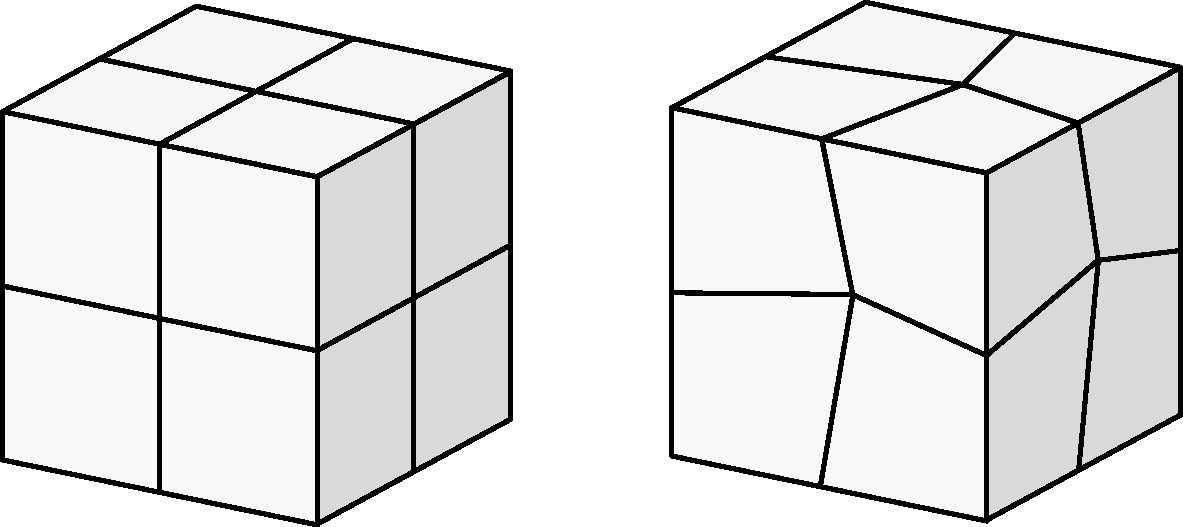
\includegraphics[width=4.0in]{figures/hexahedral_patch_meshes.pdf}
    	\caption{Hexahedral meshes: (left) regular, (right) distorted.}
    \label{fig:hexahedral_patch_meshes}
\end{figure}

\begin{figure}[!h]
    \centering
    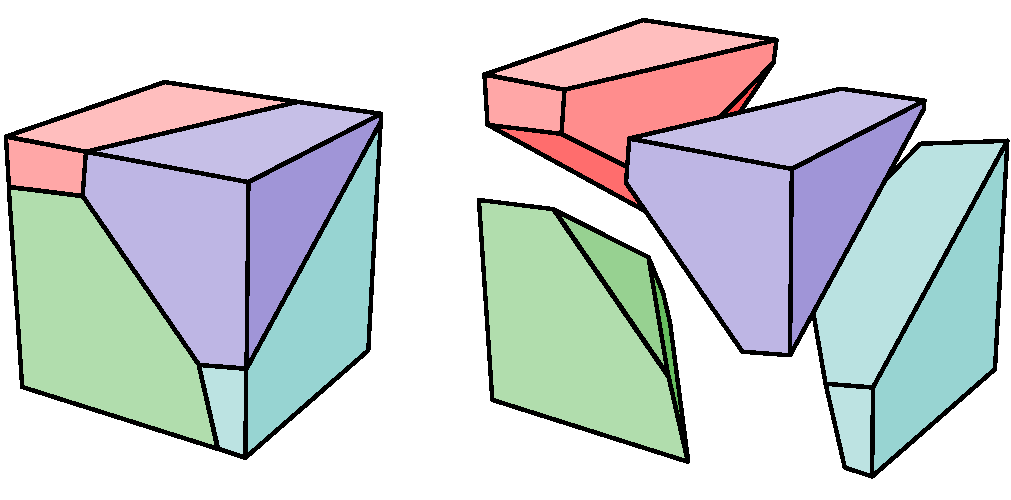
\includegraphics[width=4.0in]{figures/polyhedral_patch_mesh.pdf}
    	\caption{Patch of polyhedral elements.}
    \label{fig:polyhedral_patch_mesh}
\end{figure}

\begin{table}[!ht]
  \begin{center}
    \begin{tabular}{| l || c | c | c |}
    \hline
           & $E_1 (\Omega)$ & $||\mathbf{u}^h - \mathbf{u}|| / ||\mathbf{u}||$ & $||\boldsymbol{\sigma}^h - \boldsymbol{\sigma}|| / ||\boldsymbol{\sigma}||$ \\ \hline \hline
    FEM (regular hexahedra) & 2.4441E-016 & 1.5371E-015 & 8.1102E-016 \\ \hline
    FEM (distorted hexahedra) & 3.4394E-016 & 7.5402E-011 & 1.6047E-010 \\ \hline
    DG-PEM (no gradient correction) & 2.0369E-008 & 2.7189E-001 & 4.4846E-001 \\ \hline
    DG-PEM (symmetric correction) & 4.1522E-008 & 1.2598E-008 & 4.1608E-008 \\ \hline
    DG-PEM (nonsymmetric correction) & 2.0369E-008 & 1.0193E-008 & 2.9253E-008 \\
    \hline
    \end{tabular}
    \caption{3D linear patch test results comparison for FEM and DG-PEM.}
    \vspace{-5pt}
    \label{tab:linear_patch_test_3d}
    \vspace{-10pt}
  \end{center}
\end{table}

It is interesting to note that the FEM incurs mild errors on the distorted hexahedral mesh. Given that the elements' interpolation error remains unchanged, this error is partially attributable to inaccuracies in the numerical integration used for the elements. Using higher-order Gaussian product rules on the isoparametric elements and their faces reduces patch test errors to a limited extent. Nonetheless, some residual errors still remain.

In contrast, the accuracy of the DG-PEM appears to be limited more by interpolation error. As before, these errors are attributable to poor conditioning of the DG-PEM systems of equations. The current evidence suggests that the conditioning of $\mathbf{J}$ becomes worse in higher spatial dimensions. The use of either the symmetric or nonsymmetric gradient correction scheme assists in restoring integration consistency, yielding patch test errors on the order of $E_1 (\Omega)$.

\subsection*{Quadratic Patch Tests in 2D}

\begin{figure}[!h]
    \centering
    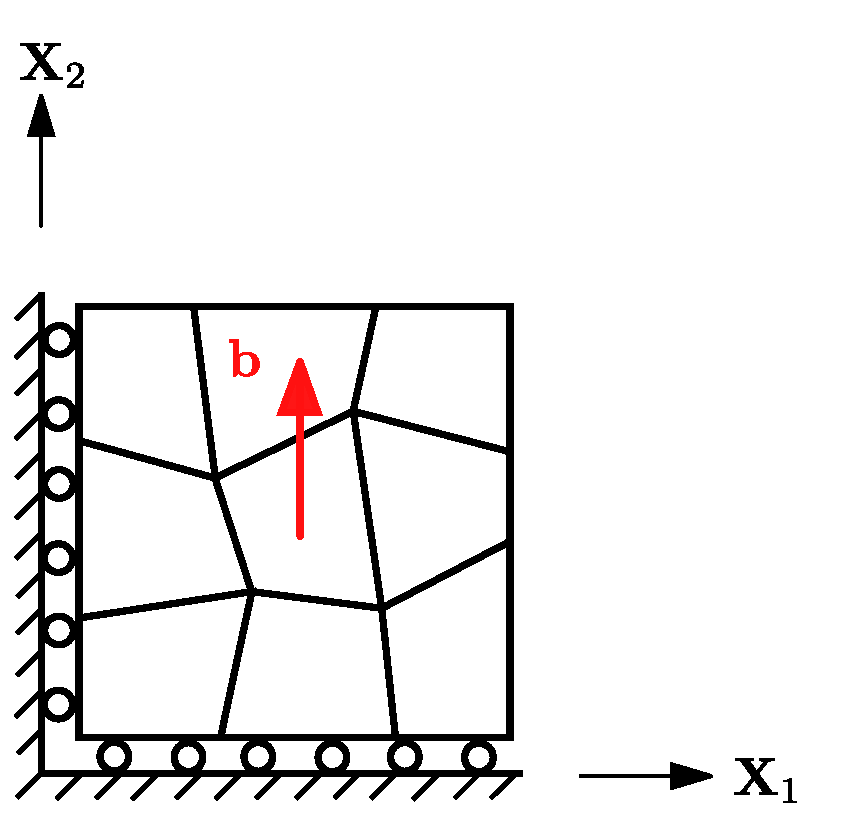
\includegraphics[width=2.5in]{figures/quadratic_patch_test.pdf}
    	\caption{Depiction of the 2D quadratic patch test.}
    \label{fig:quadratic_patch_test}
\end{figure}

Like the linear patch test, the quadratic patch test considers a similarly constrained square patch of elements, as depicted in Figure \ref{fig:quadratic_patch_test}. A constant body force $\mathbf{b} = (b_1, \, b_2)$ acts uniformly over the patch. Additionally, linearly varying tractions are applied to the unconstrained faces of the patch:
\begin{equation}
	\bar{t}_1 (X_1 = L) = - \frac{\lambda}{\lambda + 2 \mu} b_2 X_2, \quad \bar{t}_2 (X_1 = L) = 0,
\end{equation}
\begin{equation}
	\bar{t}_2 (X_2 = L) = - \frac{\lambda}{\lambda + 2 \mu} b_1 X_2, \quad \bar{t}_1 (X_2 = L) = 0.
\end{equation}
For a linear elastic material under plane strain conditions, an exact solution may be obtained of the form:
\begin{equation}
	u_1 (\mathbf{X}) = \frac{b_1}{2 (\lambda + 2 \mu)} (L - X_1) X_1 + \frac{\nu (b_1 - b_2)}{2 \mu} L X_1,
\end{equation}
\begin{equation}
	u_2 (\mathbf{X}) = \frac{b_2}{2 (\lambda + 2 \mu)} (L - X_2) X_2 + \frac{\nu (b_2 - b_1)}{2 \mu} L X_2,
\end{equation}
\begin{equation}
	\sigma_{11} (\mathbf{X}) = b_1 (L - X_1) + \frac{\lambda}{\lambda + 2 \mu} b_2 X_2,
\end{equation}
\begin{equation}
	\sigma_{22} (\mathbf{X}) = b_2 (L -  X_2) + \frac{\lambda}{\lambda + 2 \mu} b_1 X_1,
\end{equation}
\begin{equation}
	\sigma_{12} (\mathbf{X}) = 0.
\end{equation}
A special (uniaxial) case will be considered, involving only a constant body force and no boundary tractions (provided $\nu = 0$ and $b_1 = 0$):
\begin{equation}
	u_1 (\mathbf{X}) = 0, \quad u_2 (\mathbf{X}) = \frac{b_2}{2 (\lambda + 2 \mu)} (L - X_2) X_2,
\end{equation}
\begin{equation}
	\sigma_{11} (\mathbf{X}) = \sigma_{12} (\mathbf{X}) = 0, \quad \sigma_{22} (\mathbf{X}) = b_2 (L -  X_2).
\end{equation}

The two quadrilateral meshes depicted in Figure \ref{fig:quadrilateral_patch_meshes} were used in conjunction with the FEM, using both 8-node serendipity and 9-node Lagrange isoparametric formulations. The DG-PEM was used on the polygonal mesh depicted in Figure \ref{fig:quadratic_polygonal_patch_mesh}.

\begin{figure}[!h]
    \centering
    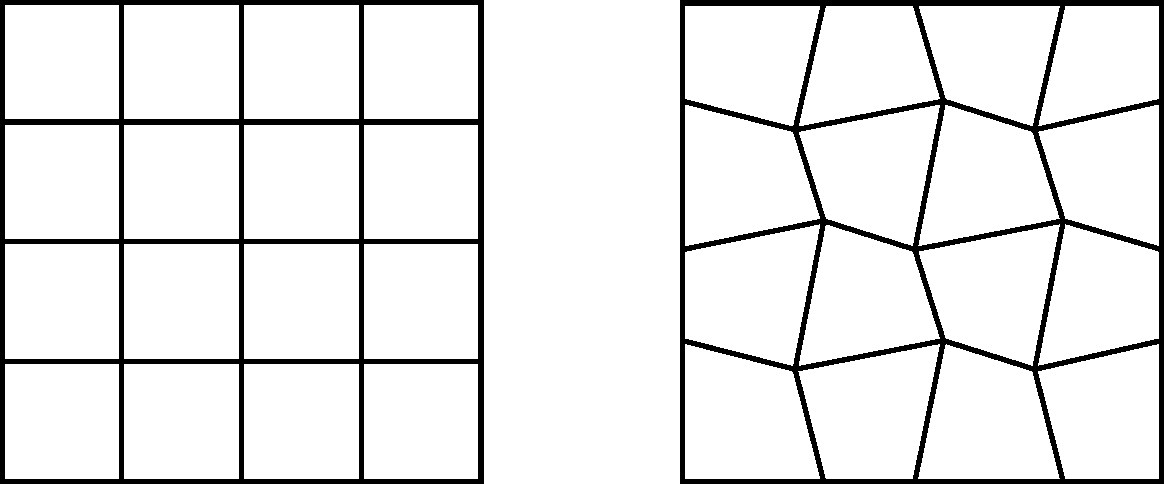
\includegraphics[width=4.0in]{figures/quadrilateral_patch_meshes.pdf}
    	\caption{Quadrilateral meshes: (left) regular, (right) distorted.}
    \label{fig:quadrilateral_patch_meshes}
\end{figure}

\begin{figure}[!h]
    \centering
    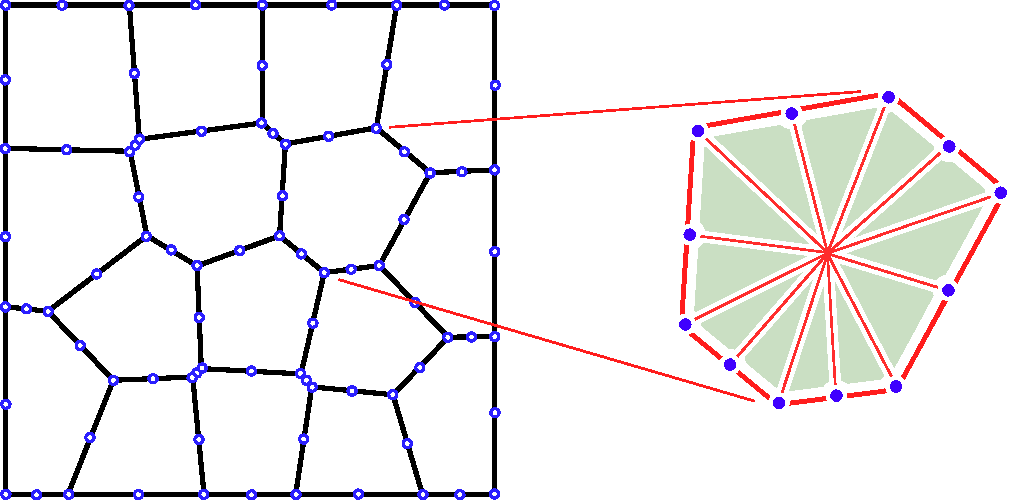
\includegraphics[width=4.0in]{figures/quadratic_polygonal_patch_mesh.pdf}
    	\caption{Patch of serendipity polygonal elements.}
    \label{fig:quadratic_polygonal_patch_mesh}
\end{figure}

Quadratic patch test errors for the FEM and DG-PEM were explored. The DG-PEM bases were chosen such that $\varphi^h \in \mathcal{D}^h_2 (\Omega)$, yielding quadratically complete shape functions. The results are presented in table \ref{tab:quadratic_patch_test}.

\begin{table}[!ht]
  \begin{center}
    \begin{tabular}{| l || c | c | c |}
    \hline
           & $E_2 (\Omega)$ & $||\mathbf{u}^h - \mathbf{u}|| / ||\mathbf{u}||$ & $||\boldsymbol{\sigma}^h - \boldsymbol{\sigma}|| / ||\boldsymbol{\sigma}||$ \\ \hline \hline
    FEM (regular 8-node quadrilaterals) & 9.0812E-016 & 1.7437E-009 & 1.3950E-008 \\ \hline
    FEM (distorted 8-node quadrilaterals) & 4.7831E-003 & 9.9714E-005 & 2.0795E-003 \\ \hline
    FEM (regular 9-node quadrilaterals) & 8.6713E-016 & 1.7437E-009 & 1.3950E-008 \\ \hline
    FEM (distorted 9-node quadrilaterals) & 1.2818E-015 & 2.0841E-009 & 1.5752E-008 \\ \hline
    DG-PEM (no gradient correction) & 3.3857E-008 & 9.8535E-002 & 2.8876E-001 \\ \hline
    DG-PEM (symmetric correction) & 3.6486E-007 & 3.5935E-008 & 1.4642E-007 \\ \hline
    DG-PEM (nonsymmetric correction) & 3.3857E-008 & 4.5498E-009 & 5.5341E-009 \\
    \hline
    \end{tabular}
    \caption{Quadratic patch test results comparison for FEM and DG-PEM.}
    \vspace{-5pt}
    \label{tab:quadratic_patch_test}
    \vspace{-10pt}
  \end{center}
\end{table}

It is interesting to note that the 8-node isoparametric quadrilaterals fail the quadratic patch test if the mesh becomes distorted. Only affinely distorted 8-node quadrilaterals will exhibit quadratic completeness. Arbitrarily distorted elements will suffer from excessive interpolation errors, as observed in Table \ref{tab:quadratic_patch_test}. This behavior is discussed in greater detail in \cite{Arnold:02} and \cite{Arnold:01}. In comparison, the 9-node quadrilateral elements preserve quadratic completeness, even when distorted as in Figure \ref{fig:quadrilateral_patch_meshes}. However, it should be remarked that if the elements' edges are curved, both the 8- and 9-node isoparametric elements will lose 2nd order completeness, and fail quadratic patch tests.

To account for the effects of integration error, the DG-PEM requires the use of a gradient correction scheme. However, if a symmetric correction scheme is employed, there is an observed loss of completeness in the representation of the solution gradients over the element, corresponding to an increase in the interpolation error. Only the nonsymmetric gradient correction method is able to achieve the desired level of accuracy in the quadratic patch test.

\subsection*{Quadratic Patch Tests in 3D}

The quadratic patch test described in the previous example may be extended directly to the 3-dimensional setting if the special (uniaxial) case is considered. As with the 3D linear patch test, the two hexahedral meshes depicted in Figure \ref{fig:hexahedral_patch_meshes} were used in conjunction with the FEM, this time using 20-node isoparametric elements. The DG-PEM was used on the ``serendipity'' polyhedral mesh depicted in Figure \ref{fig:quadratic_polyhedral_patch_mesh}, with similar parameter settings to those used for the 2D quadratic patch test. The results are displayed in Table \ref{tab:quadratic_patch_test_3d}.

\begin{figure}[!h]
    \centering
    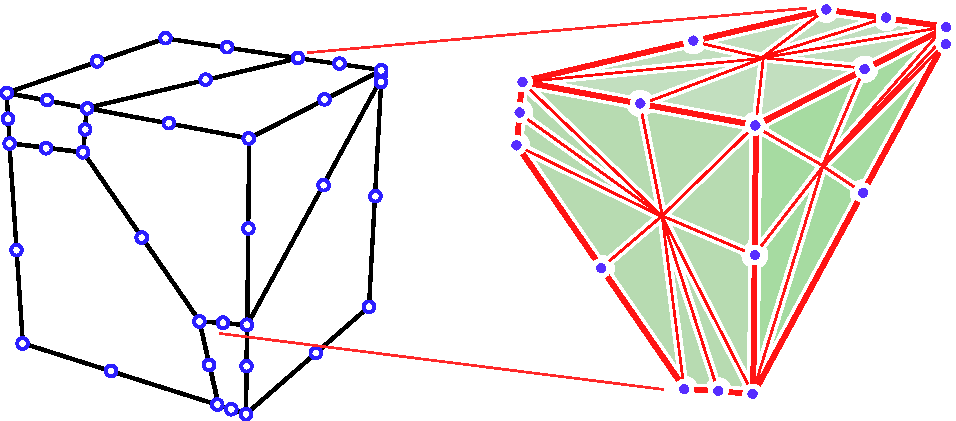
\includegraphics[width=4.0in]{figures/quadratic_polyhedral_patch_mesh.pdf}
    	\caption{Patch of serendipity polyhedral elements.}
    \label{fig:quadratic_polyhedral_patch_mesh}
\end{figure}

\begin{table}[!ht]
  \begin{center}
    \begin{tabular}{| l || c | c | c |}
    \hline
           & $E_2 (\Omega)$ & $||\mathbf{u}^h - \mathbf{u}|| / ||\mathbf{u}||$ & $||\boldsymbol{\sigma}^h - \boldsymbol{\sigma}|| / ||\boldsymbol{\sigma}||$ \\ \hline \hline
    FEM (regular hexahedra) & 6.1677E-016 & 6.9751E-009 & 2.7900E-008 \\ \hline
    FEM (distorted hexahedra) & 5.6085E-003 & 1.4755E-004 & 1.4958E-003 \\ \hline
    DG-PEM (no gradient correction) & 3.2351E-008 & 1.3054E-001 & 2.9833E-001 \\ \hline
    DG-PEM (symmetric correction) & 9.7520E-002 & 2.4536E-002 & 3.1112E-002 \\ \hline
    DG-PEM (nonsymmetric correction) & 3.2351E-008 & 2.6577E-008 & 1.1622E-008 \\
    \hline
    \end{tabular}
    \caption{3D quadratic patch test results comparison for FEM and DG-PEM.}
    \vspace{-5pt}
    \label{tab:quadratic_patch_test_3d}
    \vspace{-10pt}
  \end{center}
\end{table}

As was the case in 2D, the 20-node isoparametric brick elements perform well on the regular (undistorted) mesh, but lose polynomial completeness on the distorted mesh. Correspondingly, there is an observed loss of accuracy in both $E_2 (\Omega)$ and the patch test error metrics.

For the DG-PEM elements, an interesting phenomenon is observed with respect to the choice of gradient correction scheme. As was the case for the 2D quadratic patch test, applying a symmetric gradient correction (to both the trial and test functions) adversely impacts the polynomial completeness properties of the trial solution space. The effect is more pronounced for the 3D patch test. This result highlights the particular advantage of the nonsymmetric gradient correction scheme, which only modifies the test functions. Polynomial completeness of the trial solution space is therefore preserved, and patch test errors are rendered comparable with the (undistorted) FEM. The nonsymmetric gradient correction scheme shall therefore be used exclusively throughout the remainder of this chapter.

%Another quadratic patch test which involves no body force considers an elastic cantilever beam in pure bending, as depicted in Figure \ref{fig:bending_patch_test}. For clarity, this problem shall be referred to as the ``bending patch test.'' The support conditions of the (weakly) fixed beam are
%\begin{equation}
%	u_1 (X_1 = 0) = 0, \quad u_2 (X_1 = 0, X_2 = 0) = 0.
%\end{equation}
%A linearly varying traction $\bar{\mathbf{t}} = (M X_2, \, 0)$ is applied to the free end of the beam. For plane strain isotropic elasticity, the exact solution is:
%\begin{equation}
%	u_1 (\mathbf{X}) = \frac{M (\lambda + 2 \mu)}{4 \mu (\lambda + \mu)} X_1 X_2,
%\end{equation}
%\begin{equation}
%	u_2 (\mathbf{X}) = - \frac{M}{8 \mu (\lambda + \mu)} \left[ (\lambda + 2 \mu) X_1^2 + \lambda X_2^2 \right],
%\end{equation}
%\begin{equation}
%	\sigma_{11} = M X_2, \quad \sigma_{22} = \sigma_{12} = 0.
%\end{equation}

\section{Tests for Element Quality}

The primary advantage of partitioned element methods is that they allow for the elements to take on virtually arbitrary shape. However, elements with non-convex or degenerate features may degrade the overall accuracy of the resulting numerical solution. The motivation for the present study is to assess the effects of element formulation upon a given element's susceptibility to geometric locking phenomena.

Heuristically: an element will be more sensitive to the effects of locking if its local stiffness matrix contains a number of eigenmodes (modes of deformation) whose corresponding eigenvalues are excessively large in comparison with the low-order (affine) deformation modes. In turn, meshes containing such elements will likewise possess several high-energy modes of deformation, contributing to the phenomenon of ``mesh locking.''

As a separate issue from locking, if a given element's local stiffness matrix is poorly conditioned, the global stiffness matrix of a mesh which contains said element may become poorly conditioned, as well. This may negatively impact the degree of solution accuracy that can be obtained due to floating point arithmetic. For implicit solid mechanics applications, the accuracy of any linear solver (whether direct or iterative) will be compromised by poor conditioning of the global stiffness matrix.

With these considerations borne in mind, several tests are conducted to examine the eigenvalue spectra of individual element stiffness matrices using varying element formulations and parameter settings. The eigenvalue spectra of several global stiffness matrices for polygonal meshes of variable quality are considered, as well.

\subsection*{Conditioning of Individual Element Stiffness Matrices}

This section attempts to characterize the behavior of a representative sampling of polygonal PEM elements by examining the eigenvalues of each element's elastic stiffness matrix.

For the elements considered, a comparison study is carried out to examine differences in the eigenvalue spectra of elements whose stiffness matrices were computed using various element formulations. Specifically, approximations to harmonic shape functions were obtained for each element using the CG-PEM, the DG-PEM, and a contemporary variant of the VETFEM arising from (\ref{eq:vetfem}). These results are compared against a computed reference solution for the harmonic shape functions.

For each element, the elastic constants for Young's modulus and Poisson's ratio are chosen as $E = 1.0$ and $\nu = 0.0$, respectively. The choice of $\nu = 0.0$ is deliberate, and aims to decouple the effects of volumetric locking from the effects of geometric locking. For the purposes of comparison, all elements have roughly unit diameter.

\subsubsection*{Examination of the Effects of Geometric Non-convexity}

A study was carried out to assess the effects of geometric non-convexity on a given element's eigenvalue spectrum. Three element shapes are considered, including: (A) a regular convex polygon, (B) an element with two collinear edges, and (C) a non-convex polygon. These elements are illustrated in Figure \ref{fig:concave_element_shapes}.

\begin{figure}[!h]
  \centering
  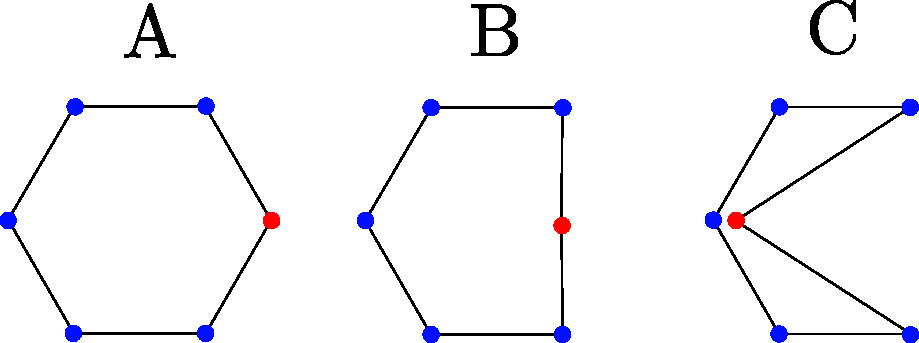
\includegraphics[width=3.5in]{figures/concave_element_shapes.pdf}  \caption{A representative sampling of hexagonal elements: (A) strictly convex, (B) two collinear edges, (C) non-convex.}
  \label{fig:concave_element_shapes}
\end{figure}

The harmonic shape functions defined on these elements were approximated using the VETFEM, the CG-PEM, and the DG-PEM. The VETFEM approximations consisted of 4th order polynomials, and were obtained as the solutions to (\ref{eq:vetfem}). The CG-PEM and DG-PEM approximations were obtained using the random Delaunay partitions shown in Figure \ref{fig:concave_element_partitions}. The penalty parameters appearing in (\ref{eq:penalty_parameters}) for the DG-PEM were chosen such that $\alpha_{\gamma0} = 10$, $\alpha_{\gamma1} = 0$ for all segments $\gamma$. Unless otherwise noted, the NIPG version of the DG-PEM (with $\epsilon = +1$) was utilized throughout. Reference solutions for the harmonic shape functions were computed on a highly refined partition of the element using the CG-PEM.

\begin{figure}[!h]
  \centering
  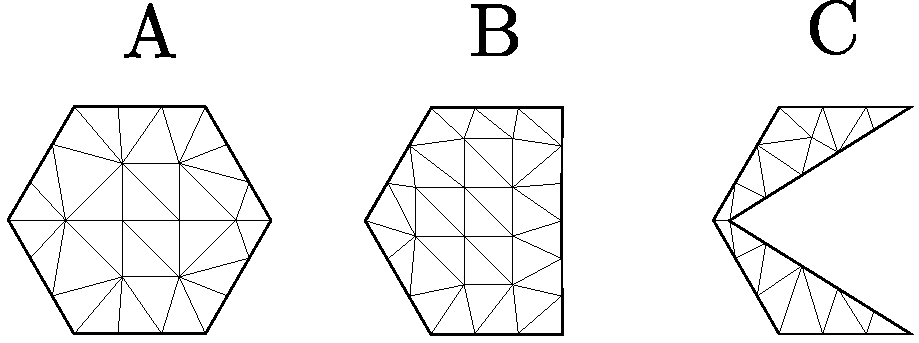
\includegraphics[width=3.5in]{figures/concave_element_partitions.pdf}  \caption{Delaunay partitions for elements A, B, and C.}
  \label{fig:concave_element_partitions}
\end{figure}

For the red nodes indicated in Figure \ref{fig:concave_element_shapes}, color plots of the associated harmonic shape functions (and their corresponding approximations) are provided in Figure \ref{fig:concave_element_comparison}.

\begin{figure}[!h]
  \centering
  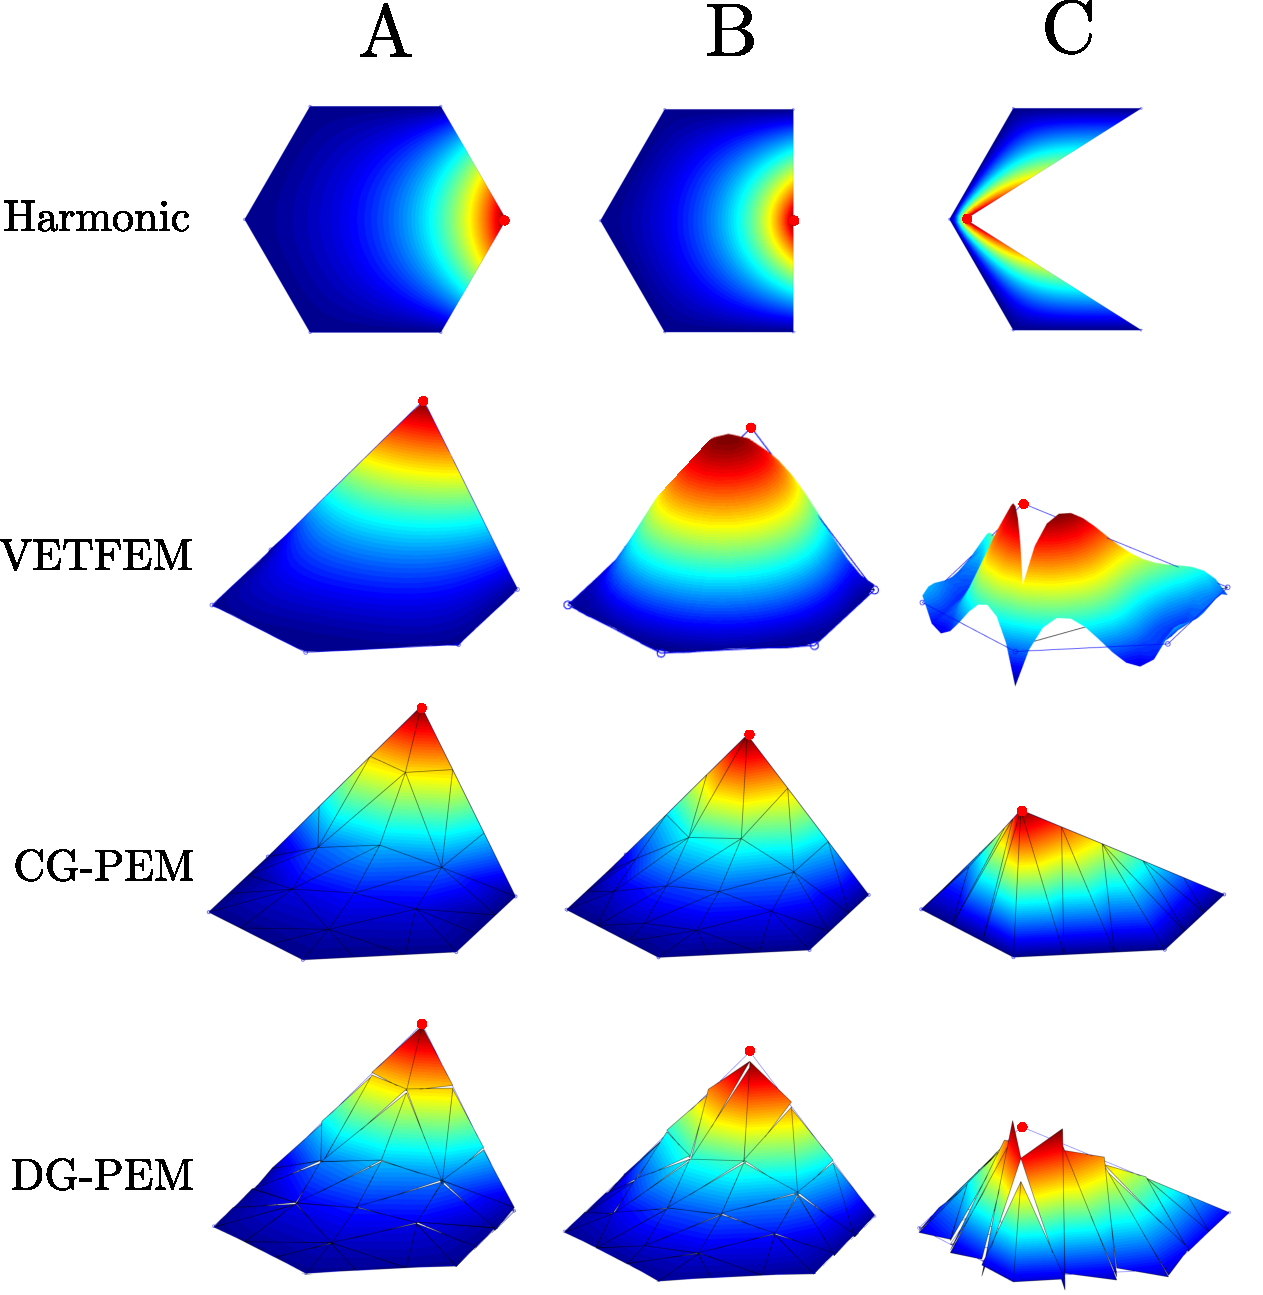
\includegraphics[width=5.0in]{figures/concave_element_comparison.pdf}  \caption{Comparison of the shape functions computed for elements A, B, and C using the VETFEM, CG-PEM, and DG-PEM.}
  \label{fig:concave_element_comparison}
\end{figure}

Concerning the VETFEM approximations depicted in Figure \ref{fig:concave_element_comparison} (particularly for elements B and C), the resulting shape functions present a number of undesirable features: oscillations, non-positivity, and non-interpolatory behavior. By comparison, the DG-PEM approximations avoid the issue of oscillations, though they are not strictly positive, nor are they interpolatory. Only the CG-PEM approximations can claim good behavior on all three fronts: they are non-oscillatory, strictly positive, and interpolatory. Nonetheless, it is important to emphasize that the aforementioned properties are not strictly necessary for convergence of the overall method. So long as a stable and consistent integration of the weak form is obtained, convergence is achieved. For certain applications, maintaining strict positivity or continuity of the shape function approximations may be desirable, though such applications are not considered here.

Using the aforementioned approximations in place of the harmonic shape functions, the elements' elastic stiffness matrices were computed (by numerical quadrature). The eigendecomposition of each element's local stiffness matrix was then determined, with particular attention paid to the largest eigenvalue $\lambda_{\max}$ and the smallest (non-zero) eigenvalue $\lambda_{\min}$. A comparison of the computed values for $\lambda_{\max}$ and $\lambda_{\min}$ is provided in table \ref{tab:concave_stiffness_max_min_eigenvalue}.

\begin{table}
\centering
\begin{subtable}{.5\textwidth}
\centering
\begin{tabular}{| c || c | c | c |}
    \hline
		Element  & A      & B      & C \\ \hline \hline
		Harmonic	 & 0.9635 & 1.2151 & 7.1166 \\ \hline
		VETFEM	 & 0.9950 & 4.4864 & 6.0305 \\ \hline
		CG-PEM	 & 1.0723 & 1.2760 & 8.7108 \\ \hline
		DG-PEM	 & 0.9668 & 1.1997 & 6.2766 \\
    \hline
    \end{tabular}
    \caption{Largest eigenvalue: $\lambda_{\max}$}
    \label{tab:concave_stiffness_max_eigenvalue}
\end{subtable}% <---- don't forget this %
\begin{subtable}{.5\textwidth}
\centering
\begin{tabular}{| c || c | c | c |}
    \hline
		Element  & A      & B      & C \\ \hline \hline
		Harmonic	 & 0.5226 & 0.3449 & 0.00562 \\ \hline
		VETFEM   & 0.5335 & 0.3491 & 0.09189 \\ \hline
		CG-PEM   & 0.6175 & 0.3935 & 0.00694 \\ \hline
		DG-PEM   & 0.5345 & 0.3425 & 0.00527 \\
    \hline
    \end{tabular}
    \caption{Smallest (non-zero) eigenvalue: $\lambda_{\min}$}
    \label{tab:concave_stiffness_min_eigenvalue}
\end{subtable}

\caption{Comparison of maximum and minimum (non-zero) eigenvalues of the element stiffness matrices for the elements shown in Figure \ref{fig:concave_element_shapes}.}
\label{tab:concave_stiffness_max_min_eigenvalue}
\end{table}

Irrespective of the chosen approximation method, the condition number for a given element's stiffness matrix becomes large as the degree of geometric non-convexity increases. The VETFEM yields a fairly accurate approximation for the eigenvalues of element A, but obtains an overly stiff approximation for element B, and overestimates the eigenvalues at the low end of the spectrum for element C. The CG-PEM appears to uniformly over-estimate the eigenvalue spectra of all elements A, B, and C (though not significantly). By contrast, the DG-PEM under-estimates the eigenvalues for elements B and C, though this behavior is observed to be contingent upon upon how the penalty parameters $\alpha_{\gamma0}$ and $\alpha_{\gamma1}$ are specified. Table \ref{tab:concave_stiffness_max_min_eigenvalue_parameter_study} illuminates the dependence of $\lambda_{\max}$ and $\lambda_{\min}$ (for element C) upon the choice of DG-PEM penalty parameters. Similar parameter dependencies are obtained for elements A and B.

\begin{table}
\centering
\begin{subtable}{1.0\textwidth}
\centering
\begin{tabular}{| l || c | c | c | c |}
    \hline
DG-PEM & $\alpha_{\gamma0} = 10^{-3}$ & $\alpha_{\gamma0} = 10^{0}$ & $\alpha_{\gamma0} = 10^{3}$ & $\alpha_{\gamma0} = 10^{6}$ \\ \hline \hline
$\alpha_{\gamma1} = 0.0$	& 5.9210 & 5.4949 & 8.6484 & 8.7108 \\ \hline
$\alpha_{\gamma1} = 10^{0}$ & 5.9210 & 5.2235 & 7.7525 & 8.7106 \\ \hline
$\alpha_{\gamma1} = 10^{3}$ & 5.9210 & 5.0938 & 3.9671 & 7.7874 \\ \hline
$\alpha_{\gamma1} = 10^{6}$ & 5.9210 & 5.0935 & 3.8699 & 3.9640 \\
    \hline
    \end{tabular}
    \caption{Largest eigenvalue: $\lambda_{\max}$}
    \label{tab:concave_stiffness_max_eigenvalue_parameter_study}
\end{subtable}% <---- don't forget this %
\\
\begin{subtable}{1.0\textwidth}
\centering
\begin{tabular}{| l || c | c | c | c |}
    \hline
DG-PEM & $\alpha_{\gamma0} = 10^{-3}$	&	$\alpha_{\gamma0} = 10^{0}$	&	$\alpha_{\gamma0} = 10^{3}$	&	$\alpha_{\gamma0} = 10^{6}$ \\ \hline \hline
$\alpha_{\gamma1} = 0.0$	&	0.004747	&	0.003554	&	0.006920	&	0.006943 \\ \hline
$\alpha_{\gamma1} = 10^{0}$	&	0.004748	&	0.003675	&	0.006489	&	0.006941 \\ \hline
$\alpha_{\gamma1} = 10^{3}$	&	0.004748	&	0.004210	&	0.002898	&	0.006508 \\ \hline
$\alpha_{\gamma1} = 10^{6}$	&	0.004748	&	0.004211	&	0.003660	&	0.002896 \\
    \hline
    \end{tabular}
    \caption{Smallest (non-zero) eigenvalue: $\lambda_{\min}$}
    \label{tab:concave_stiffness_min_eigenvalue_parameter_study}
\end{subtable}

\caption{Comparison of maximum and minimum (non-zero) eigenvalues of the element stiffness matrix for element C, computed for various DG-PEM penalty parameter values.}
\label{tab:concave_stiffness_max_min_eigenvalue_parameter_study}
\end{table}

The eigenvalue spectrum obtained for the DG-PEM converges to that of the CG-PEM as the value of $\alpha_{\gamma0}$ is increased (provided $\alpha_{\gamma1}$ is sufficiently small). Moreover, the shape functions will themselves converge to the $C^0$ continuous approximations obtained by the CG-PEM. Additionally, if $\alpha_{\gamma0}$ is made sufficiently small, the eigenvalues will becomes relatively insensitive to the choice of $\alpha_{\gamma1}$. 

Conversely, as $\alpha_{\gamma0}$ is increased, the eigenvalues (and the corresponding shape function approximations) become more sensitive to the choice of $\alpha_{\gamma1}$. In such cases, $\alpha_{\gamma1}$ may be thought of as a ``regularization'' parameter, acting to effectively smooth out variations in the gradient of the shape functions over the element. For low-order DG-PEM, increasing $\alpha_{\gamma1}$ tends the element towards a uniform gradient formulation. Doing so risks rank-deficiency of the element's resulting stiffness matrix. If $\alpha_{\gamma0}$ and $\alpha_{\gamma1}$ are increased proportionally to one another, one recovers the behavior of the pure penalty DG-PEM corresponding to (\ref{eq:pure_penalty}).

\subsubsection*{Examination of the Effects of Nearly Degenerate Features}

A study was carried out to assess the effects of geometric degeneracy on a given element's eigenvalue spectrum. The two elements illustrated in Figure \ref{fig:degenerate_element_shapes} are considered: a regular pentagon, and an irregular pentagon with a comparatively short edge.

\begin{figure}[!h]
  \centering
  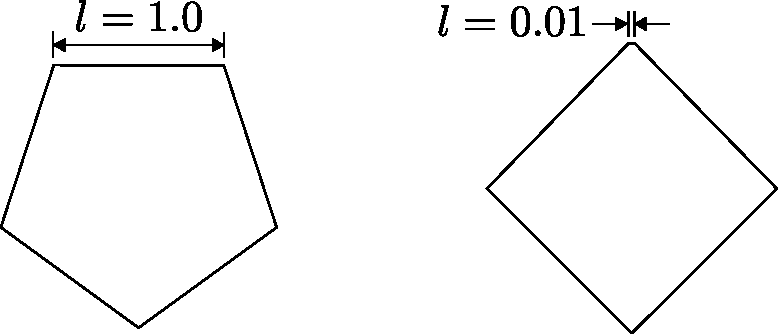
\includegraphics[width=3.7in]{figures/degenerate_element_shapes.pdf}  \caption{Two convex pentagonal elements: (left) regular pentagon with edges of equal length $l = 1.0$, (right) pentagon with a comparatively short edge of length $l = 0.01$.}
  \label{fig:degenerate_element_shapes}
\end{figure}

As in the previous example, the harmonic shape functions defined on these elements were approximated by the VETFEM (using 3rd order polynomials), the CG-PEM (using an edge-based partition), and the DG-PEM (using an edge-based partition, and the parameter settings described for the previous problem). Reference solutions for the harmonic shape functions were computed on a highly refined partition of the element using the CG-PEM.

\begin{figure}[!h]
  \centering
  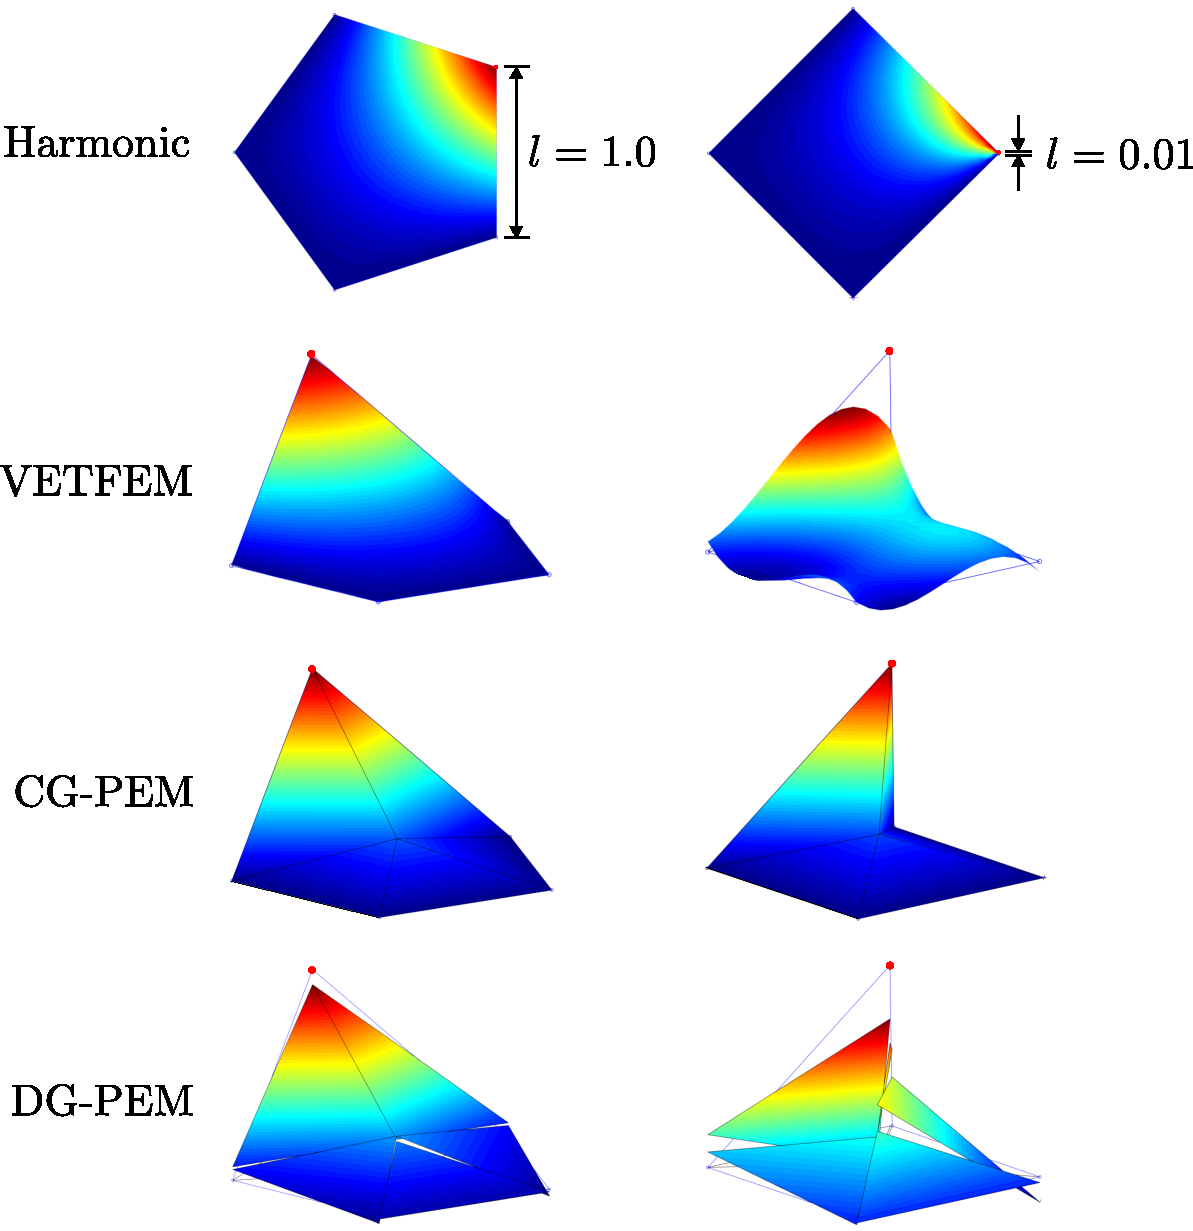
\includegraphics[width=5.0in]{figures/degenerate_element_comparison.pdf}  \caption{Comparison of shape functions computed for the two pentagonal elements with $l=1.0$ and $l=0.01$ using VETFEM, CG-PEM, and DG-PEM.}
  \label{fig:degenerate_element_comparison}
\end{figure}

As in the previous example, the aforementioned approximations were used in place of the harmonic shape functions when integrating the elements' elastic stiffness matrices. A comparison of the computed values for $\lambda_{\max}$ and $\lambda_{\min}$ is provided in table \ref{tab:degenerate_stiffness_max_min_eigenvalue}.

\begin{table}
\centering
\begin{subtable}{.5\textwidth}
\centering
\begin{tabular}{| c || c | c |}
    \hline
             & $l=1.0$ & $l=0.01$ \\ \hline \hline
    Harmonic & 0.9510 & 5.0899 \\ \hline
    VETFEM   & 0.9510 & 1.6818 \\ \hline
    CG-PEM   & 1.1326 & 64.098 \\ \hline
    DG-PEM   & 0.9510 & 1.3085 \\
    \hline
    \end{tabular}
    \caption{Largest eigenvalue: $\lambda_{\max}$}
    \label{tab:degenerate_stiffness_max_eigenvalue}
\end{subtable}% <---- don't forget this %
\begin{subtable}{.5\textwidth}
\centering
\begin{tabular}{| c || c | c |}
    \hline
             & $l=1.0$ & $l=0.01$ \\ \hline \hline
    Harmonic & 0.4925 & 0.3951 \\ \hline
    VETFEM   & 0.4906 & 0.3746 \\ \hline
    CG-PEM   & 0.8387 & 0.5516 \\ \hline
    DG-PEM   & 0.4739 & 0.2592 \\
    \hline
    \end{tabular}
    \caption{Smallest (non-zero) eigenvalue: $\lambda_{\min}$}
    \label{tab:degenerate_stiffness_min_eigenvalue}
\end{subtable}

\caption{Comparison of maximum and minimum (non-zero) eigenvalues of the element stiffness matrices computed for the elements shown in Figure \ref{fig:degenerate_element_shapes}.}
\label{tab:degenerate_stiffness_max_min_eigenvalue}
\end{table}

As noted in the previous example, the CG-PEM consistently over-estimates the eigenvalue spectra of the elements. Using a coarse (edge-based) partition further degrades the accuracy of the CG-PEM shape functions, to the extent that higher-order modes of deformation are severely over-stiff. Upon decreasing the edge length $l$ further, the maximum eigenvalue was observed to increase as $\lambda_{\max} \approx O (l^{-1})$. By comparison, the eigenvalue spectra for the VETFEM and DG-PEM remain small (well-conditioned), and relatively constant as $l \rightarrow 0$. The VETFEM, however, is observed to yield oscillatory solutions for the shape functions with decreasing $l$.

It remains to be seen whether the aforementioned insensitivity of the DG-PEM's eigenvalue spectra to short edges is a desirable quality. The following series of investigations seeks to evaluate the implications of this behavior for several polygonal meshes.

\subsection*{Meshes Consisting of Elements with Degenerate Edges}

The present study seeks to quantify the effects of having an over-abundance of short edges within a polygonal finite element mesh. The two square patches depicted in Figure \ref{fig:polygonal_patches} are considered, each containing 1,000 polygonal elements. Both meshes were generated using PolyMesher, a polygonal meshing tool detailed in \cite{Talischi:12}. The Voronoi mesh in Figure \ref{fig:patch_mesh} was obtained by a random point sampling process, and contains numerous elements with short edges. The mesh in Figure \ref{fig:lloyd_mesh} was obtained after 100 iterations of Lloyd's algorithm, yielding a polygonal mesh with reasonably well-proportioned elements. Additionally, any remaining short edges in the mesh of Figure \ref{fig:lloyd_mesh} were collapsed out according to the procedure described in \cite{Talischi:12}.
\begin{figure}[!h]
    \centering
    \begin{subfigure}[b]{0.49\linewidth}
            \centering
            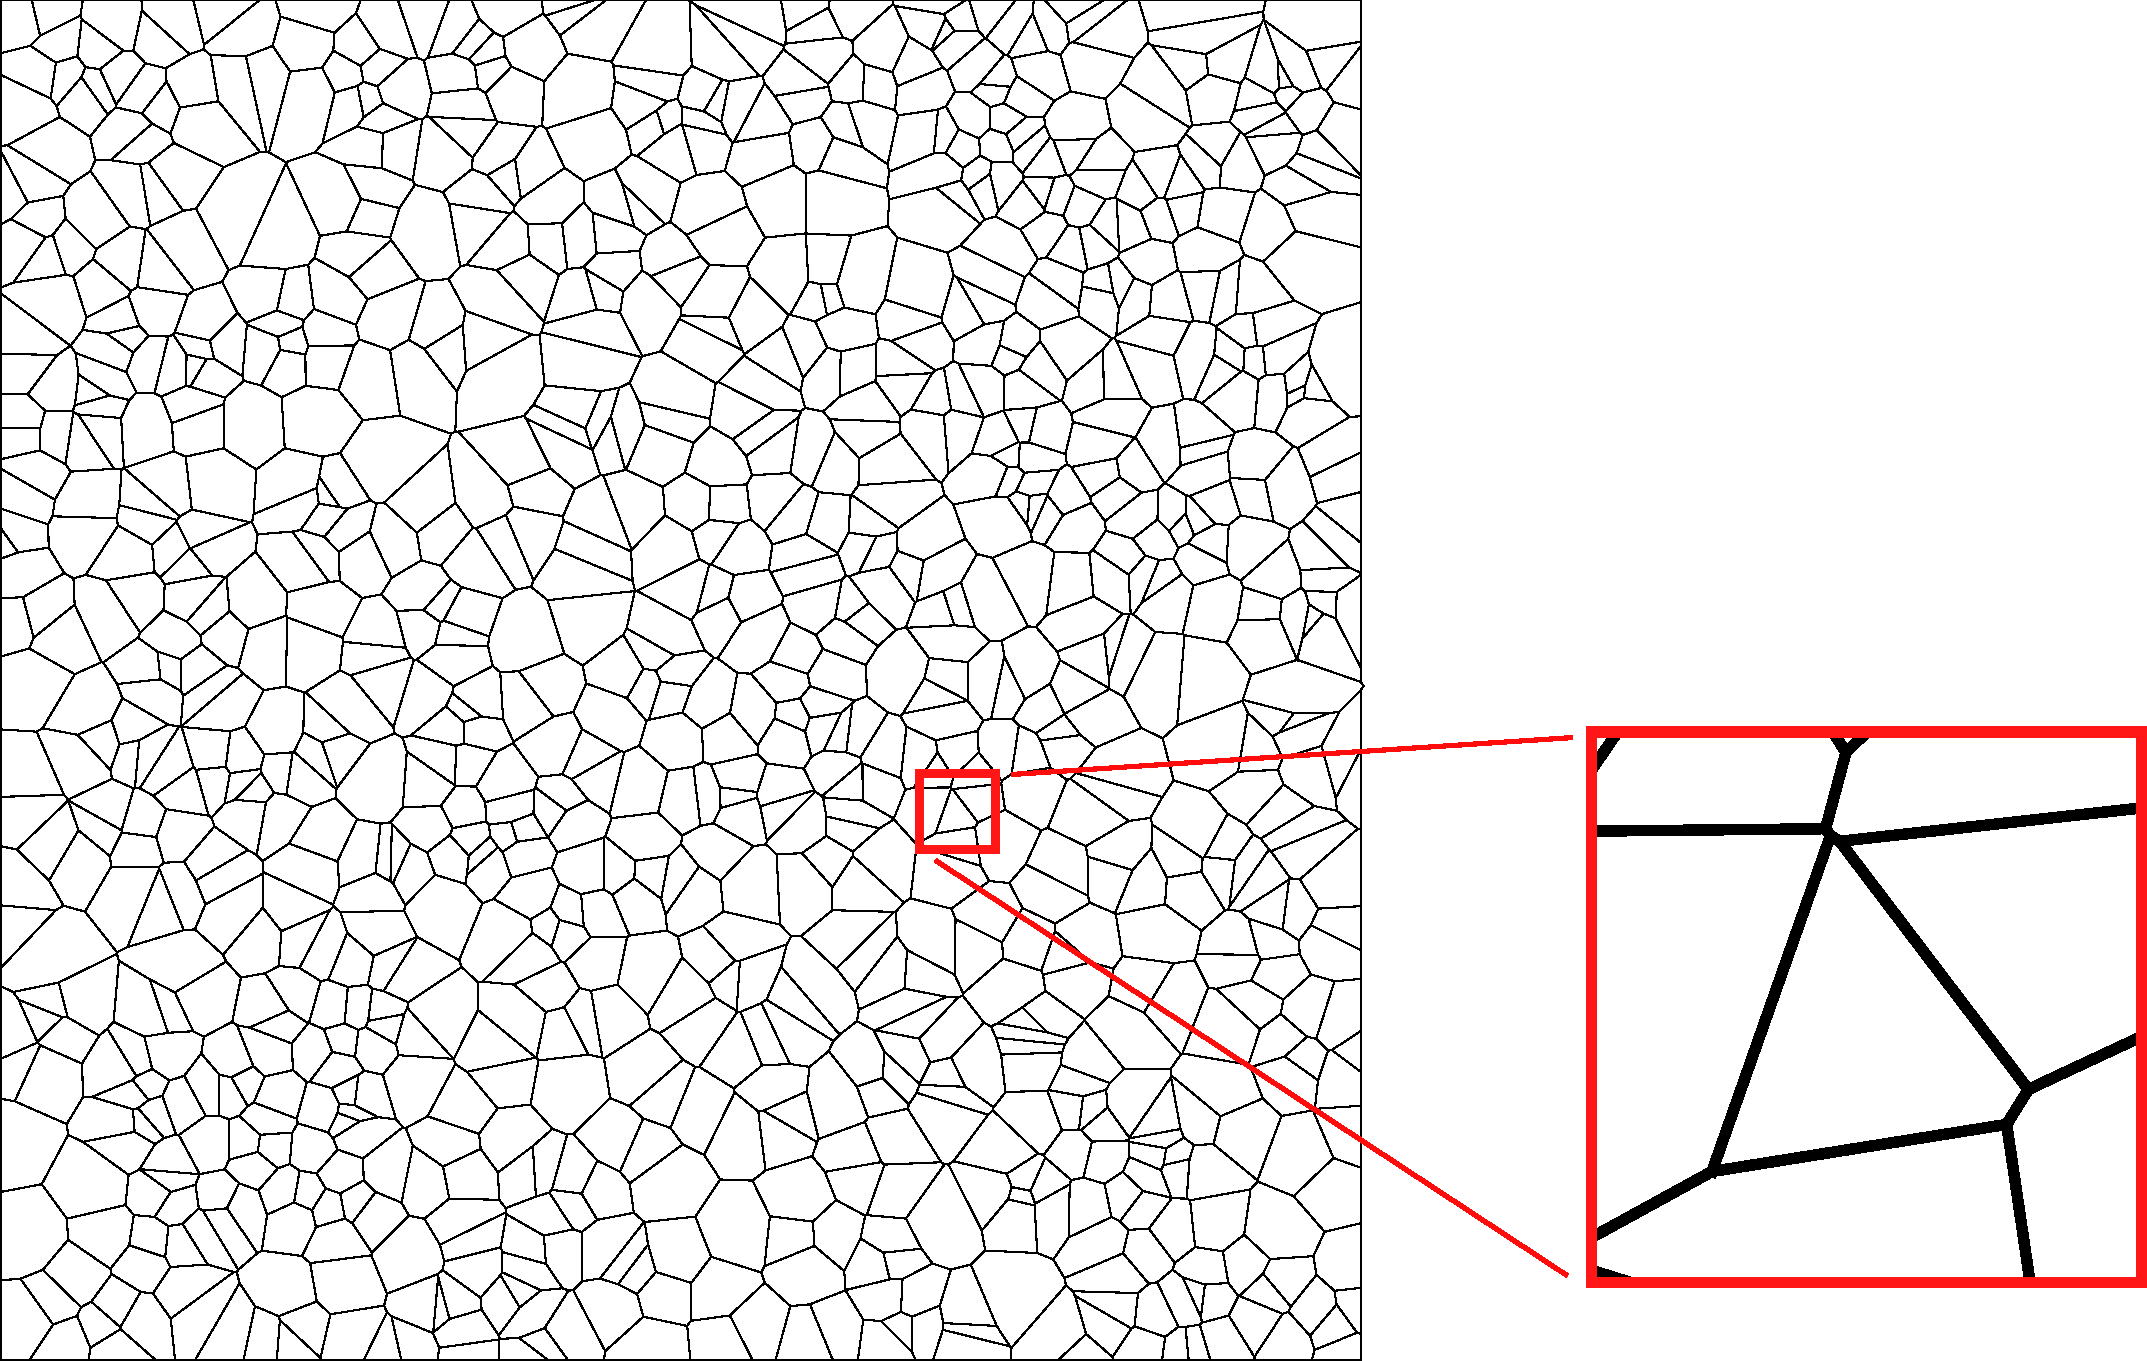
\includegraphics[width=3.0in]{figures/patch_mesh.pdf}
    			\caption{Random Voronoi mesh \label{fig:patch_mesh}}
    \end{subfigure}
	\begin{subfigure}[b]{0.49\linewidth}
            \centering
            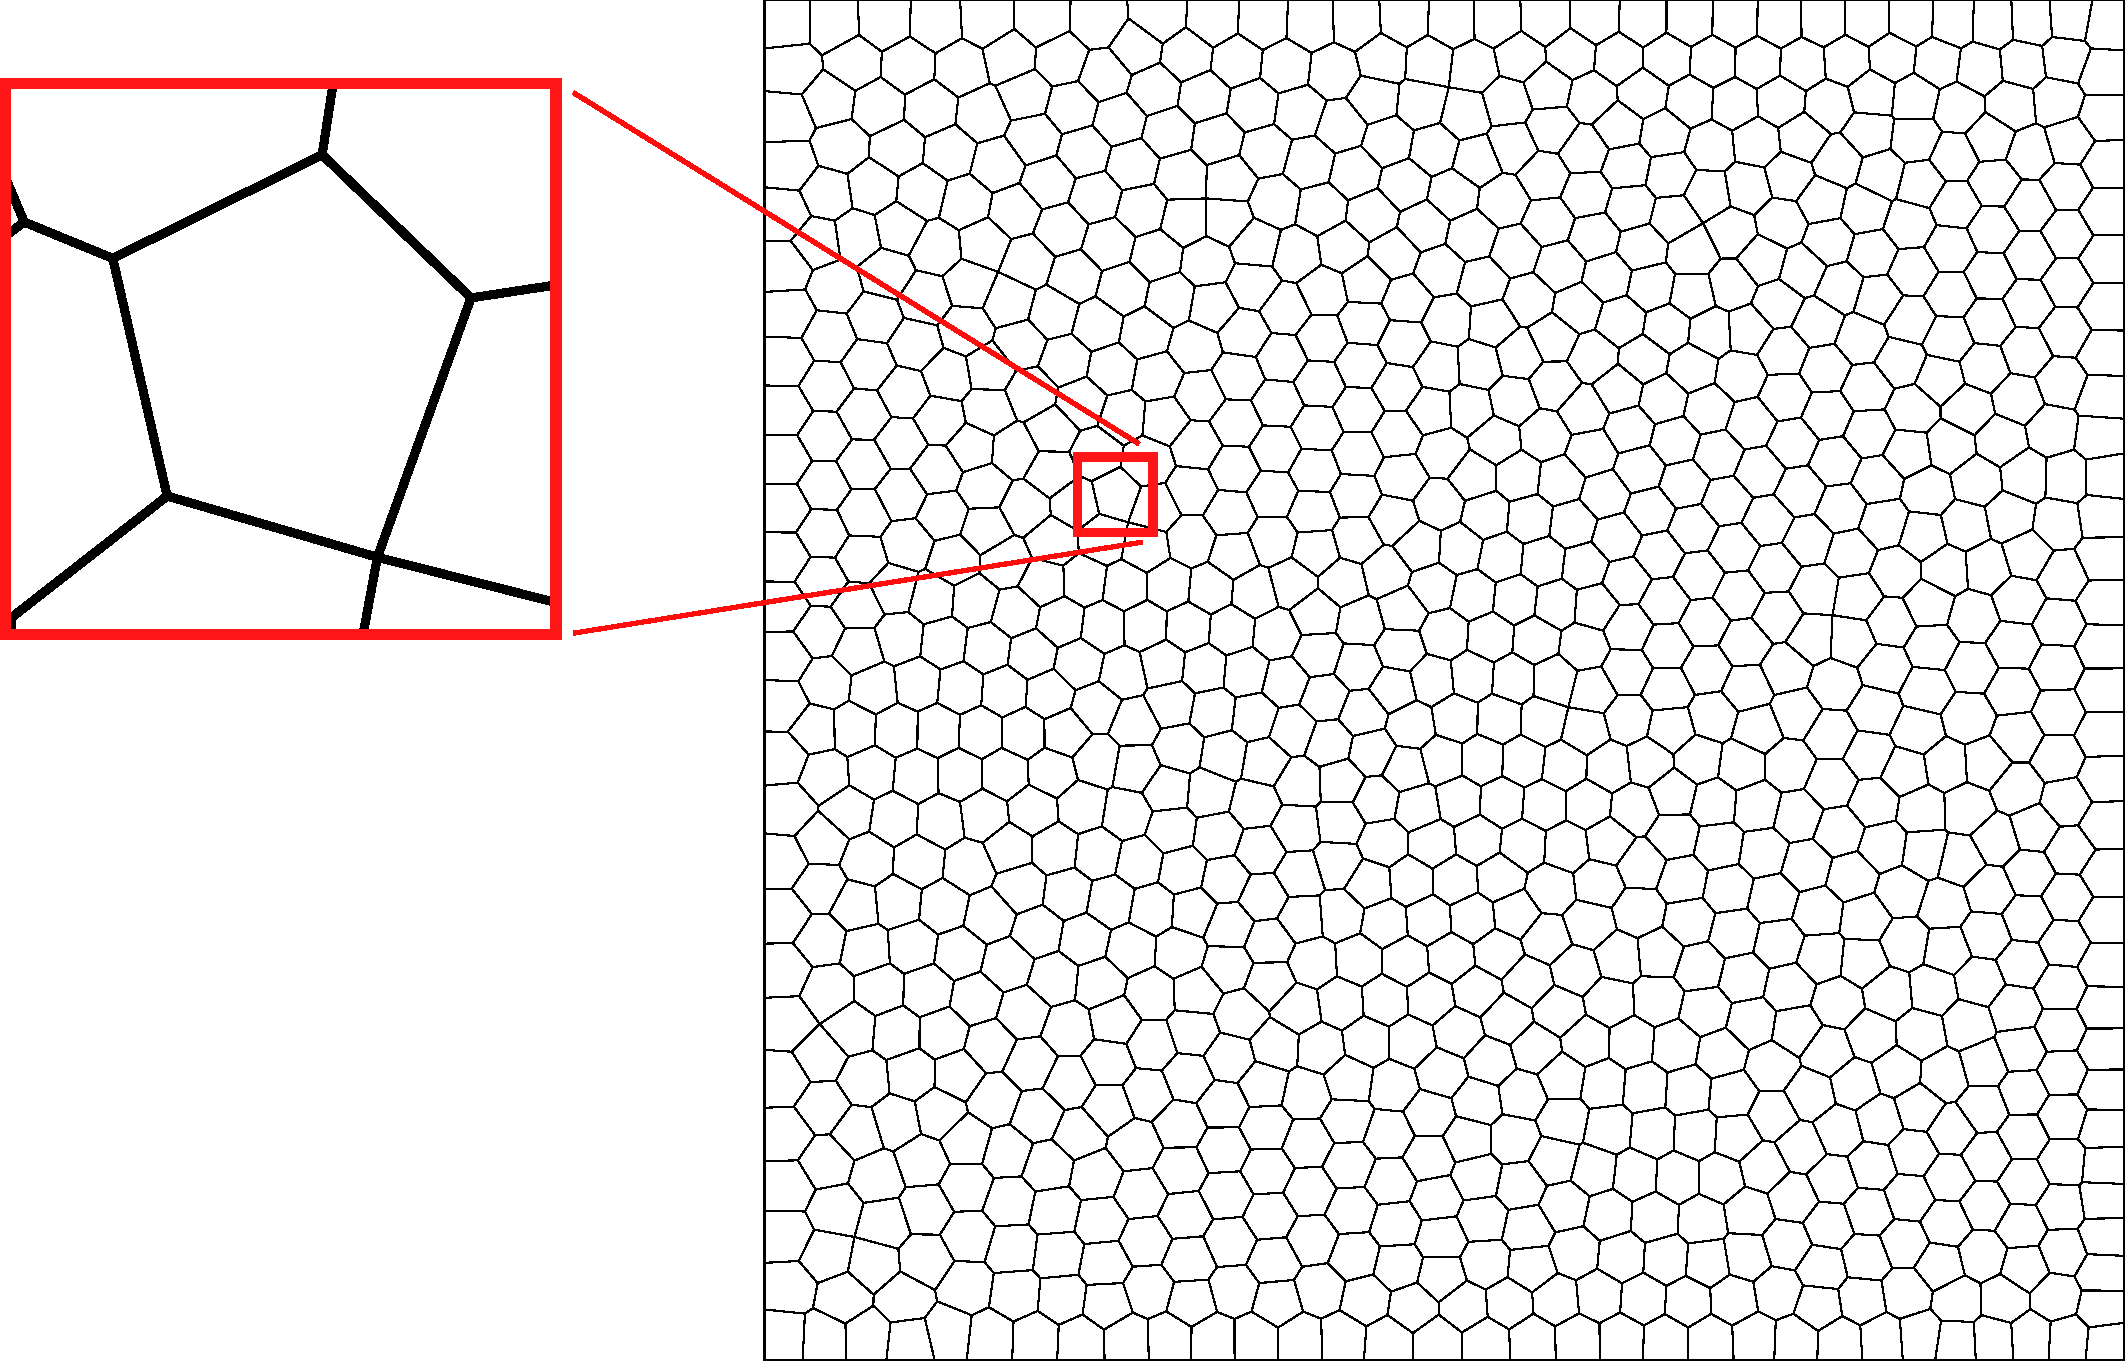
\includegraphics[width=3.0in]{figures/lloyd_mesh.pdf}
    			\caption{Lloyd mesh (100 iterations) \label{fig:lloyd_mesh}}
    \end{subfigure}
    \caption{Patches generated by PolyMesher, each containing 1,000 polygonal elements.}
    \label{fig:polygonal_patches}
\end{figure}

First, some preliminary definitions are provided for a number of relevant mesh metrics. For every polygonal element $\Omega_e \subset \mathbb{R}^2$, let $h_e$ denote the diameter of $\Omega_e$, such that
\begin{equation}
	h_e = \sup_{\mathbf{X}_1, \mathbf{X}_2 \in \Omega_e} || \mathbf{X}_1 - \mathbf{X}_2 ||_2.
\end{equation}
Further, denote by $|E|$ the length of any edge $E \subset \partial \Omega_e$, and define $\rho_e$ as the ratio of the smallest edge length $|E|$ divided by the element diameter $h_e$, i.e.
\begin{equation}
	\rho_e = \max_{E \subset \partial \Omega_e} \frac{|E|}{h_e}.
\end{equation}

For the meshes depicted in Figure \ref{fig:polygonal_patches}, the aforementioned edge length metrics were computed for all elements and edges in each mesh. Several histograms which characterize this data are provided in Figure \ref{fig:patch_edge_metrics}.
\begin{figure}[!h]
    \centering
    \begin{subfigure}[b]{0.49\linewidth}
            \centering
            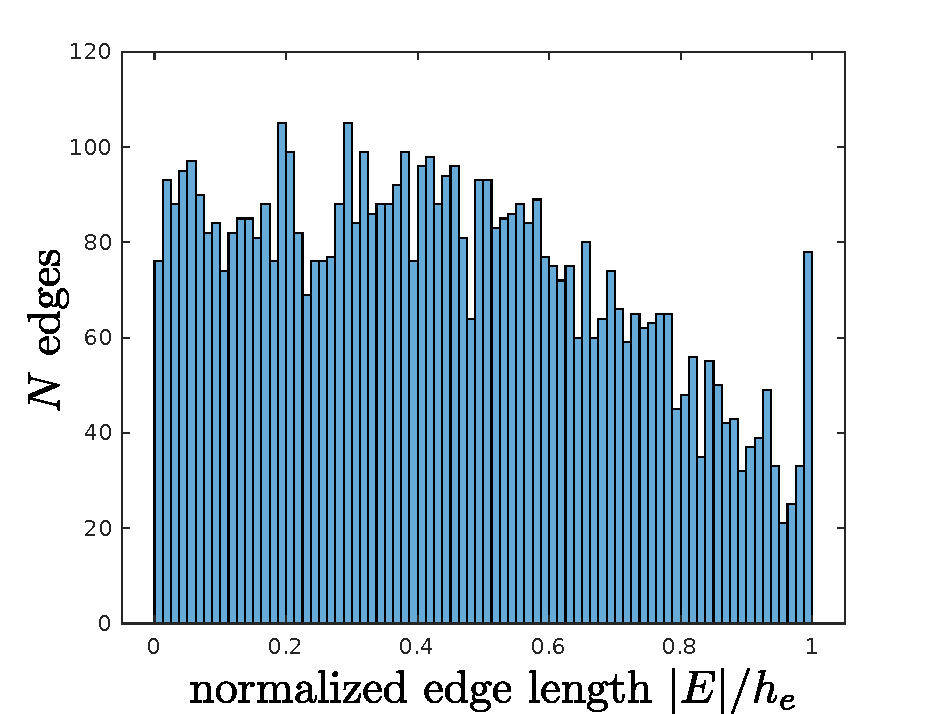
\includegraphics[width=3.0in]{figures/patch_edge_lengths.pdf}
    			\caption{Voronoi mesh \label{fig:patch_edge_lengths}}
    \end{subfigure}
	\begin{subfigure}[b]{0.49\linewidth}
            \centering
            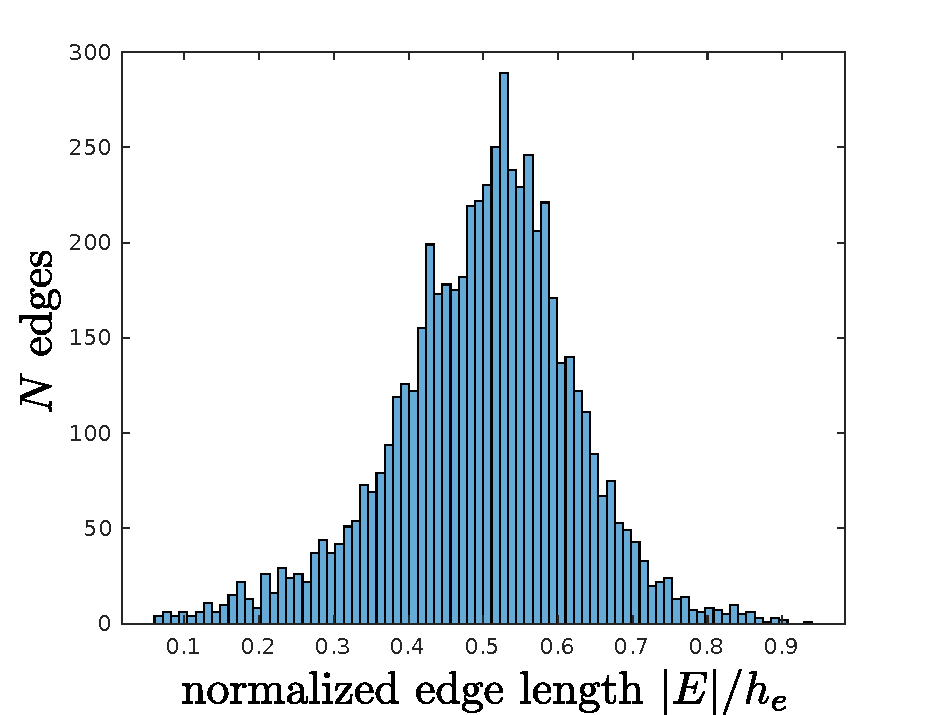
\includegraphics[width=3.0in]{figures/lloyd_edge_lengths.pdf}
    			\caption{Lloyd mesh \label{fig:lloyd_edge_lengths}}
    \end{subfigure}
    \begin{subfigure}[b]{0.49\linewidth}
            \centering
            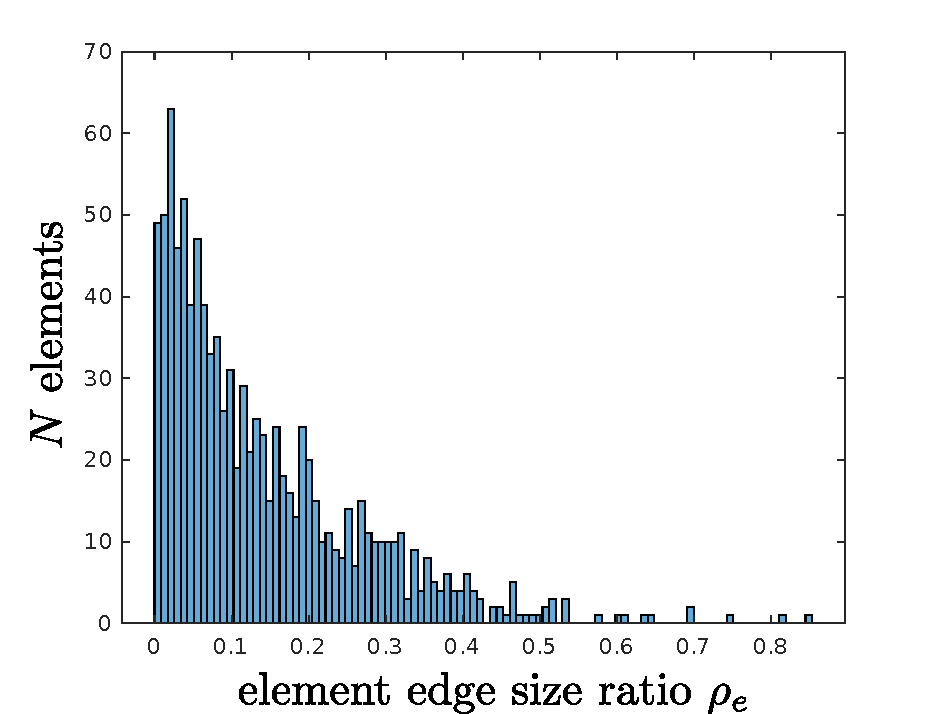
\includegraphics[width=3.0in]{figures/patch_edge_ratios.pdf}
    			\caption{Voronoi mesh \label{fig:patch_edge_ratios}}
    \end{subfigure}
	\begin{subfigure}[b]{0.49\linewidth}
            \centering
            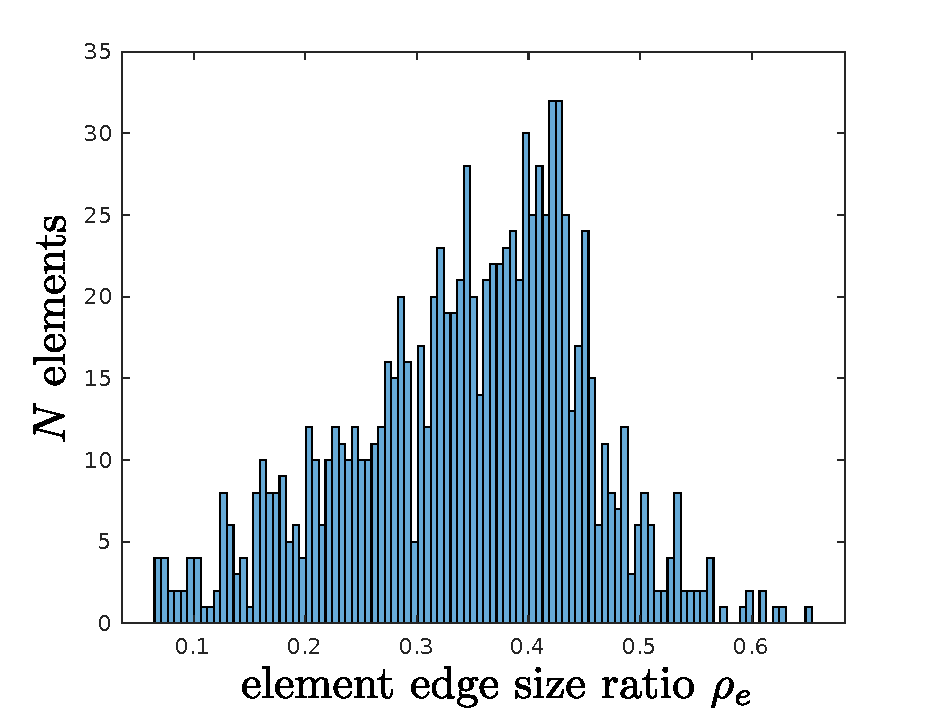
\includegraphics[width=3.0in]{figures/lloyd_edge_ratios.pdf}
    			\caption{Lloyd mesh \label{fig:lloyd_edge_ratios}}
    \end{subfigure}
    \caption{Histograms of various mesh metrics associated with the polygonal meshes depicted in Figure \ref{fig:polygonal_patches}:  (\subref{fig:patch_edge_lengths}) and (\subref{fig:lloyd_edge_lengths}) show the distributions of edge lengths contained in the random Voronoi and Lloyd meshes, respectively. (\subref{fig:patch_edge_ratios}) and (\subref{fig:lloyd_edge_ratios}) show the distributions for the smallest edge length ratios $\rho_e$ in the random Voronoi and Lloyd meshes, respectively.}
    \label{fig:patch_edge_metrics}
\end{figure}

A key observation regarding Figure \ref{fig:patch_edge_metrics} concerns the distribution of edge lengths within the random Voronoi mesh. The normalized lengths of all edges in the Voronoi mesh appear to be distributed almost uniformly, as seen in Figure \ref{fig:patch_edge_lengths}. Nonetheless, Figure \ref{fig:patch_edge_ratios} suggests that there is a relatively high probability that any given element in the random Voronoi mesh will contain at least one short edge. By comparison, the distributions for $|E|/h_e$ and $\rho_e$ in the Lloyd mesh are more Gaussian in nature, as demonstrated by Figures \ref{fig:lloyd_edge_lengths} and \ref{fig:lloyd_edge_ratios}, respectively.

To quantify the potential impact of short edges on finite element solution accuracy, the eigenvalue spectra of each patch's global stiffness matrix $\mathbf{K}$ were examined. Excessively large eigenvalues (particularly for the Voronoi mesh) may indicate solution sensitivity to the choice of discretization.

Each patch was specified to have unit dimensions ($1 \times 1$) and material properties ($E = 1.0$, $\nu = 0.0$). Global stiffness matrices were assembled for the two polygonal meshes shown in Figure \ref{fig:polygonal_patches} using the CG-PEM and the DG-PEM. Both formulations employed an edge-based partitioning scheme with composite mid-point quadrature on each element. The DG-PEM parameters were specified as $\epsilon = +1$, $\alpha_{\gamma0} = 10$, and $\alpha_{\gamma1} = 0$. The resulting eigenvalue spectra are plotted in Figure \ref{fig:patch_eigenvalue_distributions}.

\begin{figure}[!h]
  \centering
  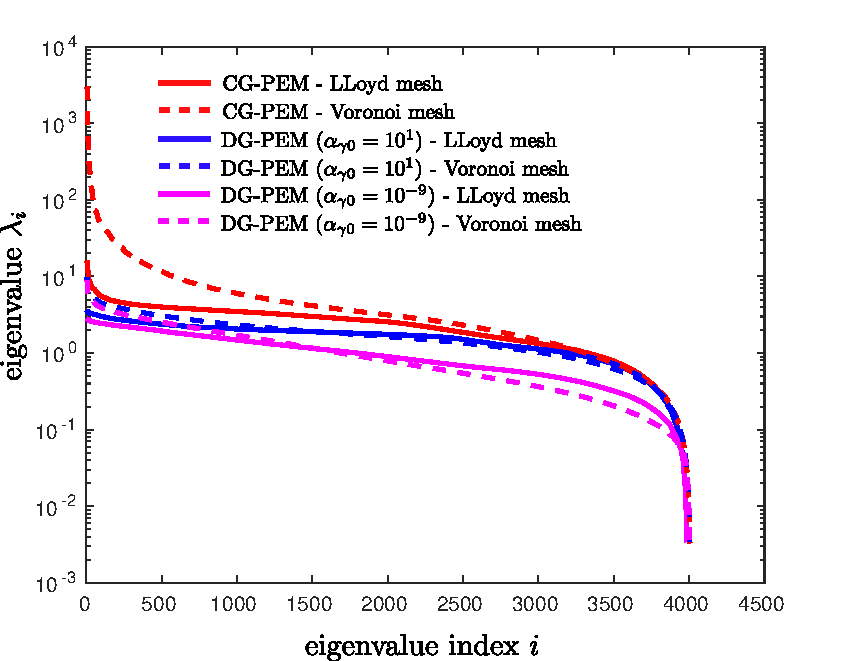
\includegraphics[width=5.0in]{figures/eigenvalue_distributions.pdf}  \caption{Eigenvalue spectra $\left\{ \lambda_i \right\}_{i = 1}^{N-3}$ for the (elastic) global stiffness matrix $\mathbf{K}$, computed for the CG-PEM and the DG-PEM ($\epsilon = +1$, $\alpha_{\gamma1} = 0$).}
  \label{fig:patch_eigenvalue_distributions}
\end{figure}

For the Lloyd mesh, both the CG-PEM and DG-PEM produce fairly comparable eigenvalue spectra. For the random Voronoi mesh, the CG-PEM produces higher-energy modes with significantly larger eigenvalues than the DG-PEM. Interestingly, the DG-PEM yields very similar eigenvalue spectra for both meshes. This appears to indicate a diminished sensitivity of the DG-PEM solution to the chosen discretization. Importantly, the behavior of the lower-energy modes remains the same across all meshes and element formulations. Figure \ref{fig:patch_eigenmodes_DGPEM} depicts the lowest-energy mode shapes determined by the DG-PEM. Similar mode shapes and corresponding eigenvalues were obtained for the CG-PEM.
\begin{figure}[!h]
  \centering
  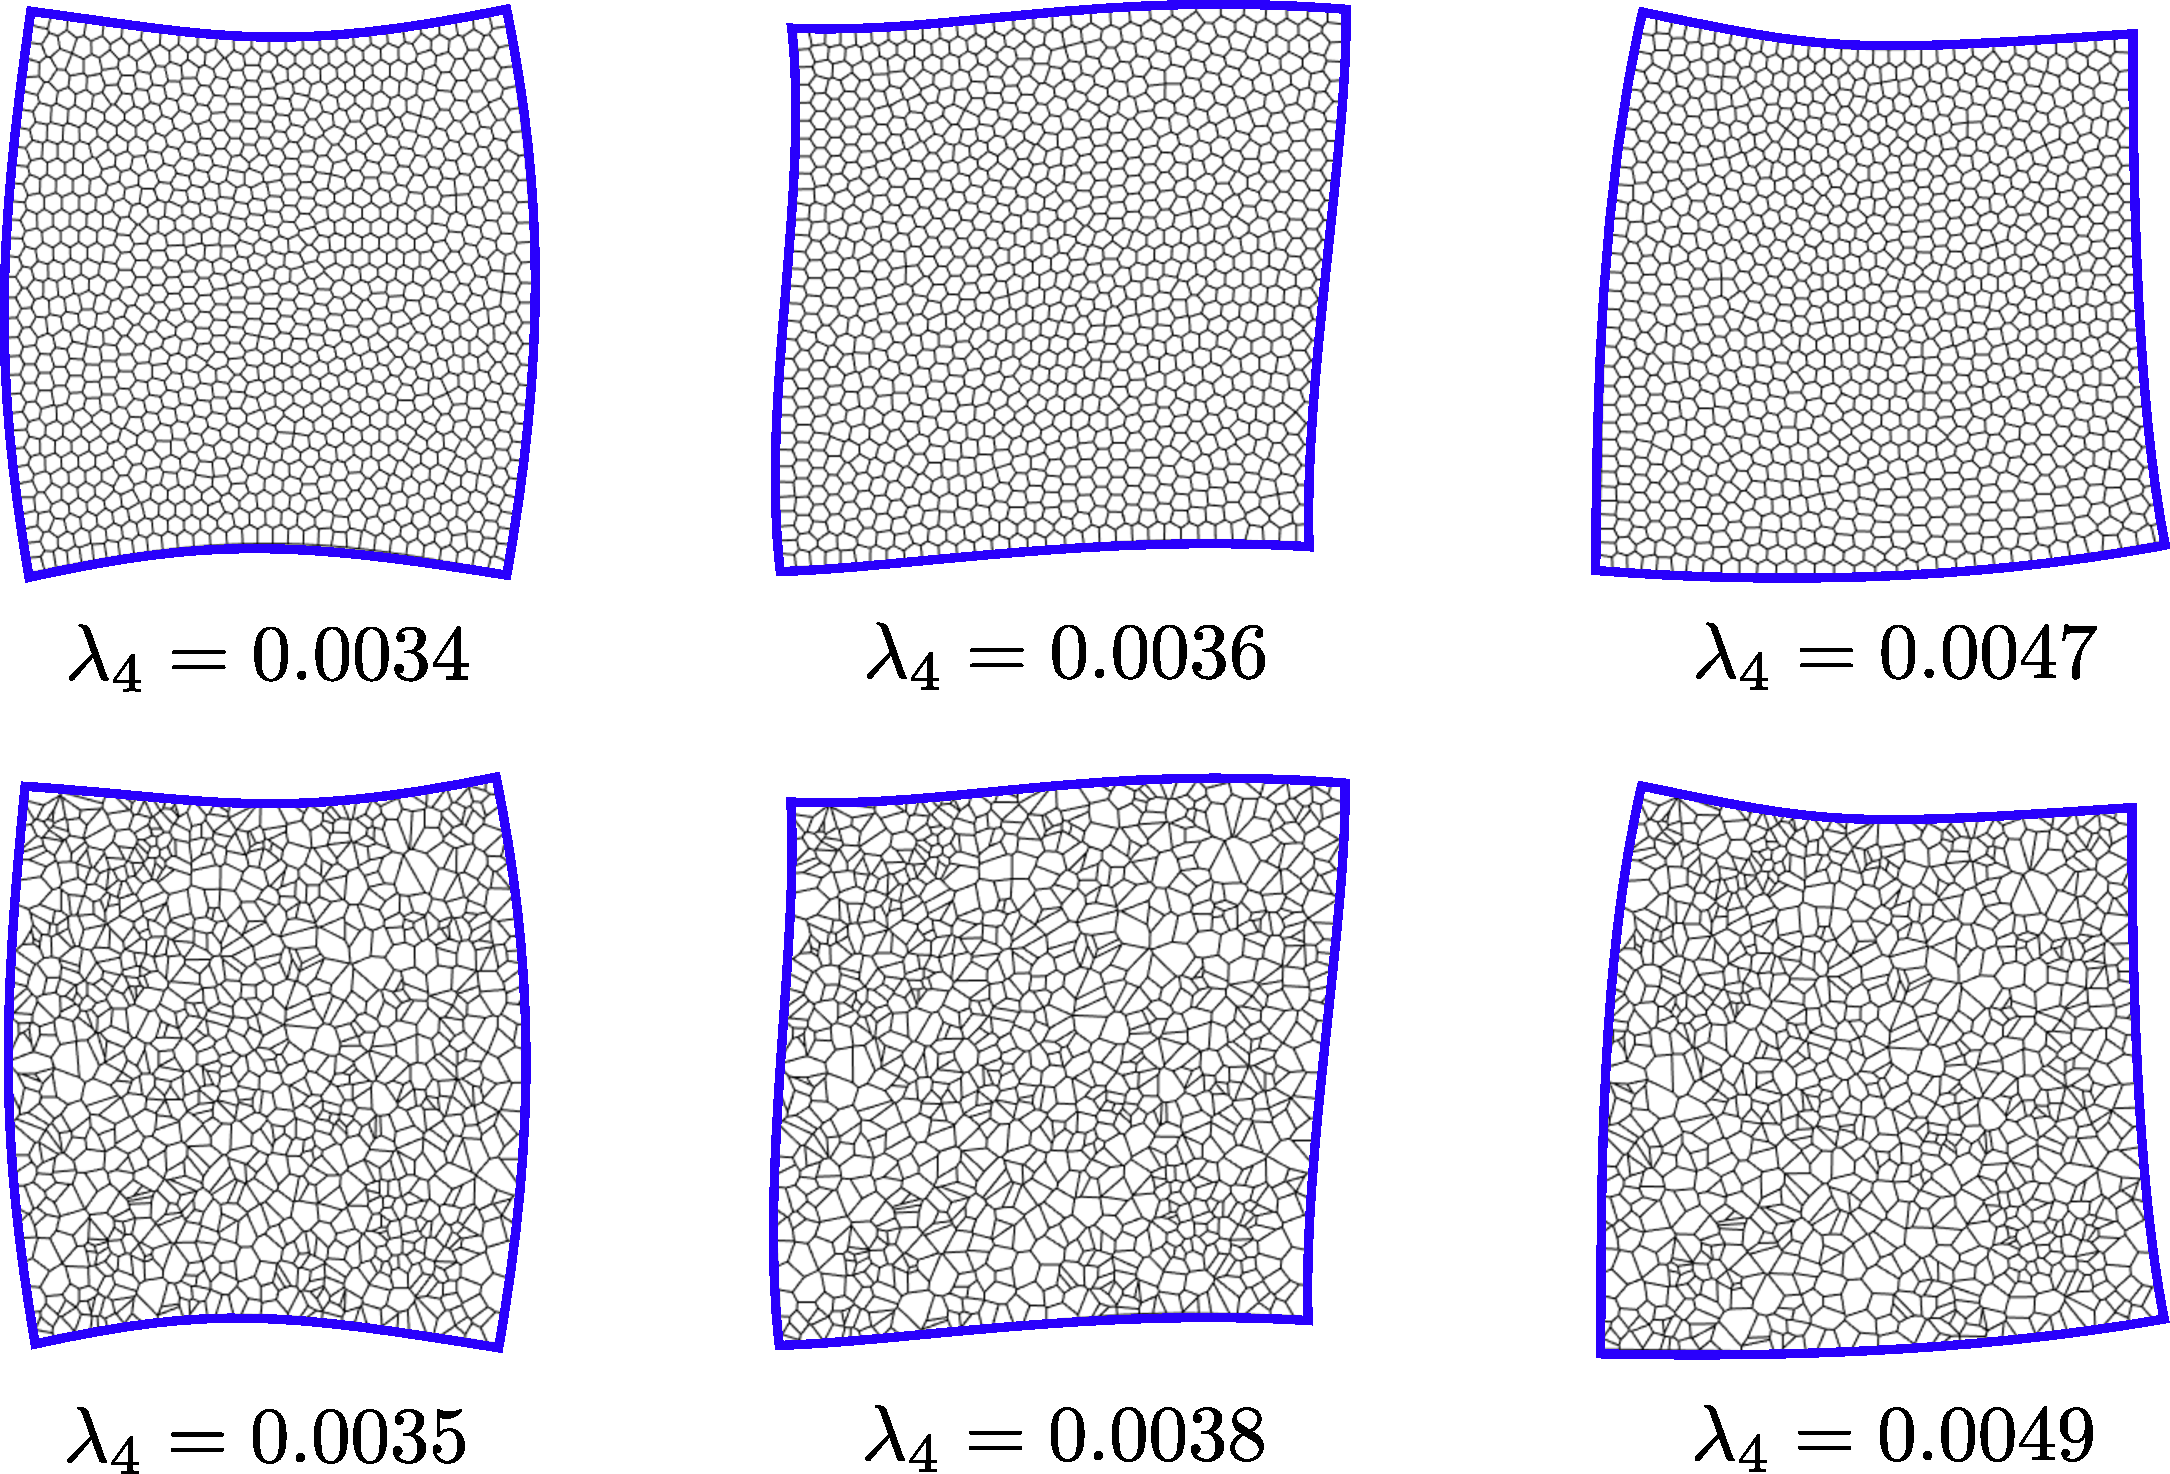
\includegraphics[width=5.0in]{figures/patch_eigenmodes_DGPEM.pdf}  \caption{Depiction of the smallest non-zero eigenvalues and corresponding eigenmodes computed using the DG-PEM ($\epsilon = +1$, $\alpha_{\gamma0} = 10$, $\alpha_{\gamma1} = 0$). $N$ denotes the size of the global stiffness matrix $\mathbf{K}$, and $\lambda_{N} = \lambda_{N-1} = \lambda_{N-2} = 0$ correspond to the zero-energy modes of deformation.}
  \label{fig:patch_eigenmodes_DGPEM}
\end{figure}

It is stressed that the results obtained for the DG-PEM will vary depending on the choice of penalty parameters $\alpha_{\gamma0}$ and $\alpha_{\gamma1}$. As $\alpha_{\gamma0} \rightarrow \infty$ the behavior of the CG-PEM is recovered. The corresponding variability in the condition number of $\mathbf{K}$ is characterized in Table \ref{tab:global_stiffness_condition_number}.
\begin{table}[!ht]
  \begin{center}
    \begin{tabular}{| l || c | c |}
    \hline
           & Voronoi mesh & Lloyd mesh \\ \hline \hline
    CG-PEM & 9.1e+05 & 4.6e+03 \\ \hline
    DG-PEM ($\alpha_{\gamma0} = 10^3$) & 4.8e+04 & 4.4e+03 \\ \hline
    DG-PEM ($\alpha_{\gamma0} = 10^1$) & 2.9e+03 & 1.0e+03 \\ \hline
    DG-PEM ($\alpha_{\gamma0} = 10^{-1}$) & 2.7e+03 & 8.1e+02  \\ \hline
    DG-PEM ($\alpha_{\gamma0} = 10^{-9}$) & 2.7e+03 & 8.1e+02 \\
    \hline
    \end{tabular}
    \caption{Computed values for the condition number $\kappa(\mathbf{K})$ of the global stiffness matrix $\mathbf{K}$ (excluding rigid body modes).}
    \vspace{-5pt}
    \label{tab:global_stiffness_condition_number}
    \vspace{-10pt}
  \end{center}
\end{table}

The condition number of the resulting global stiffness matrix will become large (asymptotically approaching that of the CG-PEM) as $\alpha_{\gamma0}$ is increased. Conversely, decreasing $\alpha_{\gamma0}$ lowers the condition number of $\mathbf{K}$, achieving an apparent lower-bound on $\kappa (\mathbf{K})$ in the limit as $\alpha_{\gamma0} \rightarrow 0$. Importantly, the resulting stiffness matrix does not contain spurious zero-energy modes, regardless of the choice of $\alpha_{\gamma0}$. Because any choice of $\alpha_{\gamma0} > 0$ yields stability, $\alpha_{\gamma0}$ should not be regarded as a type of hourglass control parameter.

% FEPEM - lloyd
% Max E = 1.6e+1
% Mix E = 3.5e-03
% E Rat = 4.6e+03

% FEPEM - patch
% Max E = 3.0e+03
% Mix E = 3.3e-03
% E Rat = 9.1e+05
% Min Emodes:  0.0034, 0.0036, 0.0047

% DGPEM - lloyd - A0 = 1.0e+3
% Max E = 1.5e+1
% Mix E = 3.5e-03
% E Rat = 4.4e+03
% Min Emodes: 0.0035, 0.0038, 0.0049

% DGPEM - patch - A0 = 1.0e+3
% Max E = 1.6e+02
% Mix E = 3.3e-03
% E Rat = 4.8e+04

% DGPEM - lloyd - A0 = 1.0e+1
% Max E = 3.6e+00
% Mix E = 3.5e-03
% E Rat = 1.0e+03

% DGPEM - patch - A0 = 1.0e+1
% Max E = 9.6e+00
% Mix E = 3.3e-03
% E Rat = 2.9e+03

% DGPEM - lloyd - A0 = 1.0e-1
% Max E = 2.8e+00
% Mix E = 3.5e-03
% E Rat = 8.1e+02

% DGPEM - patch - A0 = 1.0e-1
% Max E = 8.9e+00
% Mix E = 3.3e-03
% E Rat = 2.7e+03

%\begin{figure}[!h]
%    \centering
%    \begin{subfigure}[b]{0.49\linewidth}
%            \centering
%            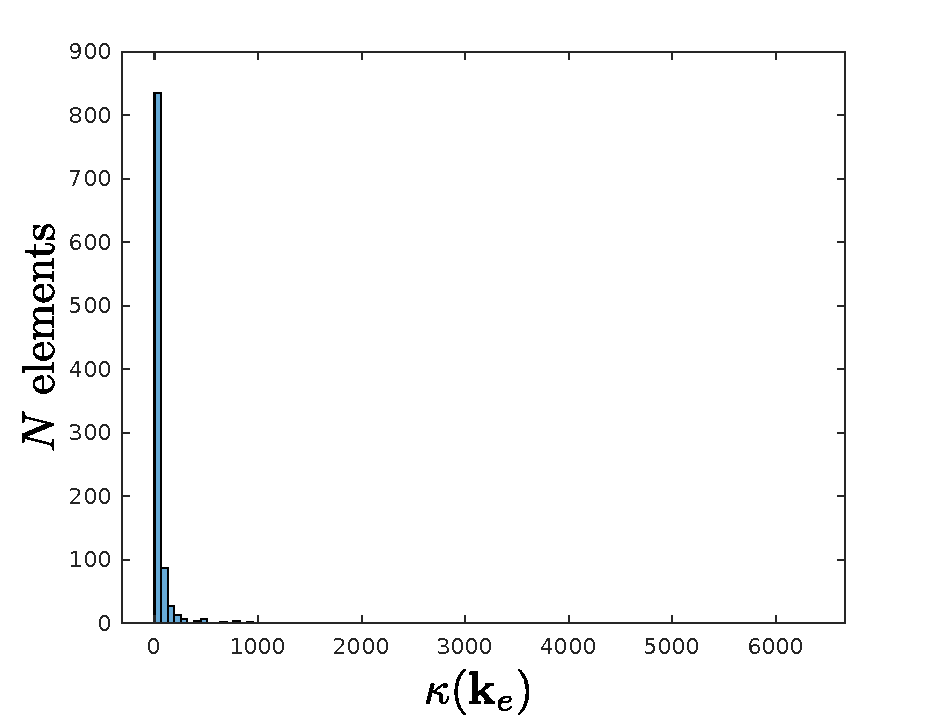
\includegraphics[width=3.0in]{figures/patch_condition_number_FEPEM.pdf}
%    			\caption{CG-PEM on the Voronoi mesh  \label{fig:patch_condition_number_FEPEM}}
%    \end{subfigure}
%	\begin{subfigure}[b]{0.49\linewidth}
%            \centering
%            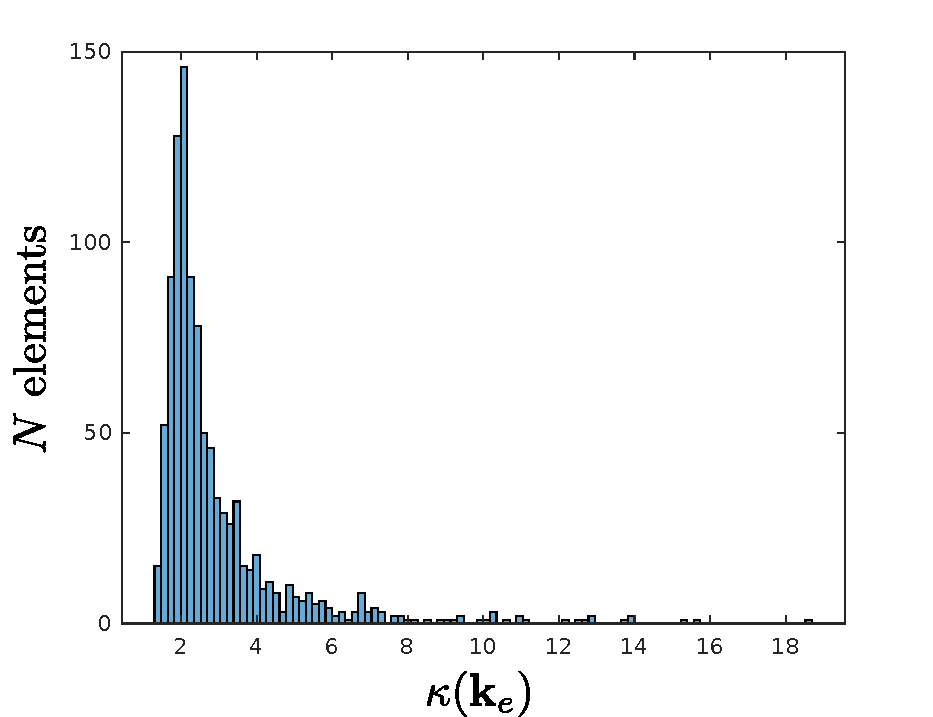
\includegraphics[width=3.0in]{figures/lloyd_condition_number_FEPEM.pdf}
%    			\caption{CG-PEM on the Lloyd mesh  \label{fig:lloyd_condition_number_FEPEM}}
%    \end{subfigure}
%    \begin{subfigure}[b]{0.49\linewidth}
%            \centering
%            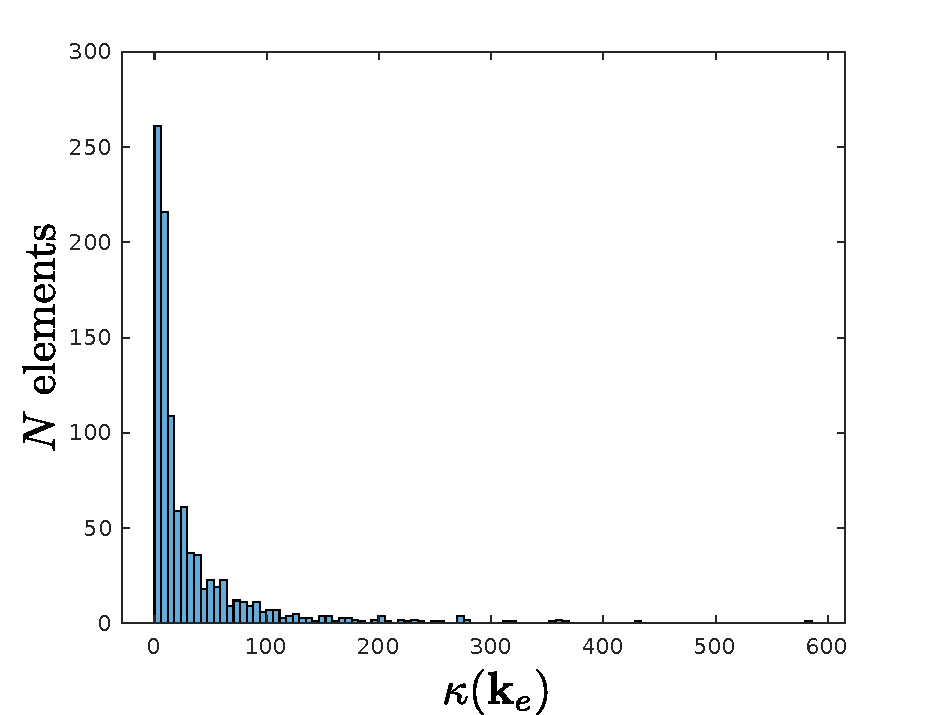
\includegraphics[width=3.0in]{figures/patch_condition_number_DGPEM.pdf}
%    			\caption{DG-PEM on the Voronoi mesh  \label{fig:patch_condition_number_DGPEM}}
%    \end{subfigure}
%	\begin{subfigure}[b]{0.49\linewidth}
%            \centering
%            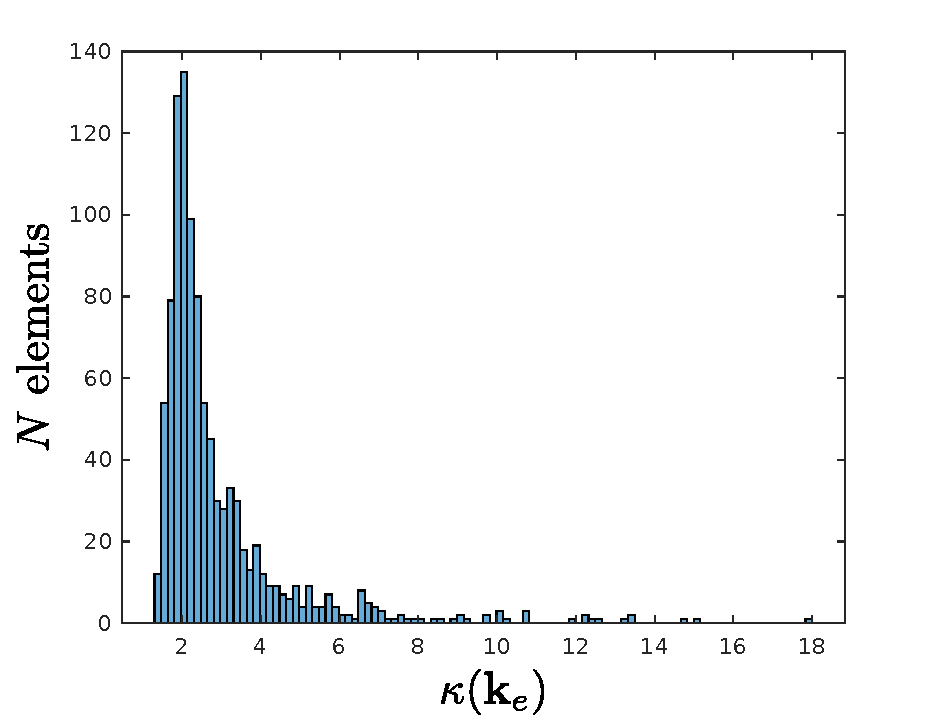
\includegraphics[width=3.0in]{figures/lloyd_condition_number_DGPEM.pdf}
%    			\caption{DG-PEM on the LLoyd mesh  \label{fig:lloyd_condition_number_DGPEM}}
%    \end{subfigure}
%    \caption{Histograms of various element metrics associated with the polygonal meshes depicted in Figure \ref{fig:polygonal_patches}:  (\subref{fig:patch_edge_lengths}) and (\subref{fig:lloyd_edge_lengths}) show the distributions of edge lengths contained in the random Voronoi and Lloyd meshes, respectively; (\subref{fig:patch_edge_ratios}) and (\subref{fig:lloyd_edge_ratios}) show the distributions for the smallest edge length ratios $\rho_e$ in the random Voronoi and Lloyd meshes, respectively.}
%\end{figure}

% local condition number investigation
	% look at DG-PEM system conditioning for certain degenerate elements
	%	* construct a random voronoi mesh on a 2d patch of elements
	%		- get edge-length metrics for voronoi cells
	%   		- examine condition number of local DGPEM systems on these elems
	%       - examine condition number of local stiffness matricies
	%			* look at max and min eigenvalues
	%		- check partition of unity and linear completeness passage
	%		- after grad correction, examine satisfaction of patch tests
	%	* do this for quadratic elements, as well
	%	* do parameter sensitivity analysis
	%	* look at global stiffness matrix condition number
	% look at conditioning for plate-like geometry (anisotropic patch tests)

% check via a series of single-element tests:
	% - examine a test involving a single non-convex element
	%   * shift node around, showing behavior vs. parameterized location
	%     - compare results for VETFEM, DGPEM, and FEPEM vs true harmonic SF
	%     - look at:
	%       * max and min eigenvalues of resulting stiffness matrix
	%       * comment on condition number, and effect on 
	%   * choose different partitioning algorithms / refinement levels
	%   * play around with DGPEM penalization parameters
	%   * examine effects of choosing DG
	% - do a test with a patch of non-convex elements
	%   * examine effects on global stiffness matrix conditioning
	%	* parameterized non-convexity, 

\section{Convergence Studies}

A handful of studies were conducted to assess the convergence behavior of the DG-PEM. These studies sought to verify that the DG-PEM yields convergent sequences of approximations under mesh refinement. A few relatively simple two- and three-dimensional elasticity problems are considered. The results obtained for the DG-PEM are compared against the results for the classical FEM. The DG-PEM employed the standard parameter settings utilized in previous problems. Convergence of both linear and quadratic PEM elements is established, and convergence in the incompressible limit is examined for discretizations consisting of hexahedra and arbitrary polyhedra.

\subsection*{Infinite Elastic Plate in Far-Field Tension}

\begin{figure}[!h]
  \centering
  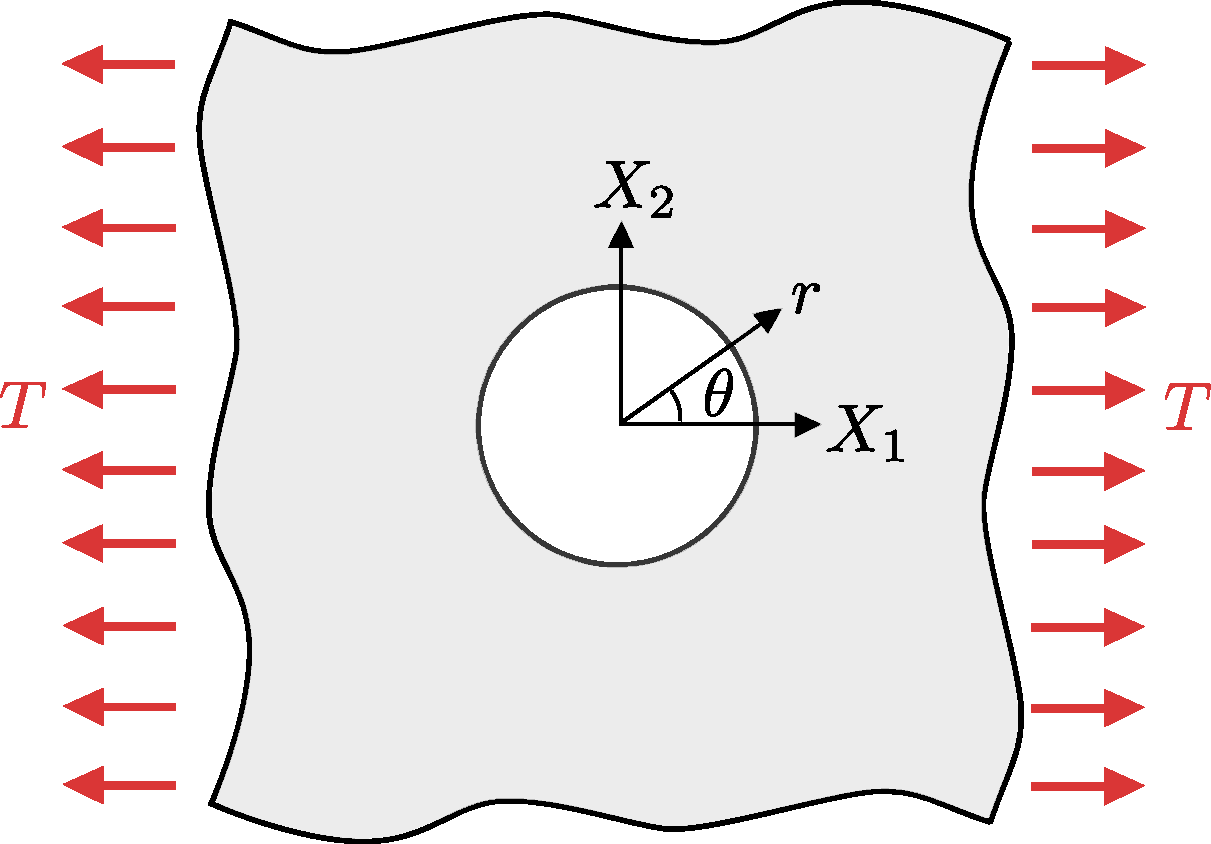
\includegraphics[width=4.0in]{figures/plate_with_hole.pdf}  \caption{Infinite plate with a circular hole placed in uniaxial tension.}
  \label{fig:plate_with_hole_problem}
\end{figure}
To demonstrate optimal convergence of the PEM for higher-order elements, consider the 2D elastostatics problem of an infinite plate with a circular hole in uniaxial tension (depicted in figure \ref{fig:plate_with_hole_problem}). The following analytical solutions for the displacement and stress fields were obtained from reference \cite{Wikiversity:17}:
\begin{equation}
  u_1 (r,\theta) = \frac{Ta}{8\mu} \left[ \frac{r}{a} (\kappa + 1) \cos \theta + \frac{2a}{r} ((1+\kappa) \cos \theta + \cos 3 \theta) - \frac{2a^3}{r^3} \cos 3 \theta \right],
\end{equation}
\begin{equation}
  u_2 (r,\theta) = \frac{Ta}{8\mu} \left[ \frac{r}{a} (\kappa - 3) \sin \theta + \frac{2a}{r} ((1-\kappa) \sin \theta + \sin 3 \theta) - \frac{2a^3}{r^3} \sin 3 \theta \right],
\end{equation}
\begin{equation}
  \sigma_{11} (r, \theta) = T - T \frac{a^2}{r^2} \bigg( \frac{3}{2} \cos 2 \theta + \cos 4 \theta \bigg) + T \frac{3a^4}{2r^4} \cos 4 \theta,
\end{equation}
\begin{equation}
  \sigma_{22} (r, \theta) = - T \frac{a^2}{r^2} \bigg( \frac{1}{2} \cos 2 \theta - \cos 4 \theta \bigg) - T \frac{3a^4}{2r^4} \cos 4 \theta,
\end{equation}
\begin{equation}
  \sigma_{12} (r, \theta) = - T \frac{a^2}{r^2} \bigg( \frac{1}{2} \sin 2 \theta + \sin 4 \theta \bigg) + T \frac{3a^4}{2r^4} \sin 4 \theta,
\end{equation}
where $T$ is the far-field value of the applied tensile stress, $a$ is the radius of the circular hole centered at $r=0$, $\kappa = 4 - 3\nu$ (under plane-strain conditions), and $\nu$ and $\mu$ are the the Poisson's ratio and shear modulus of the material, respectively.

\begin{figure}[!h]
  \centering
  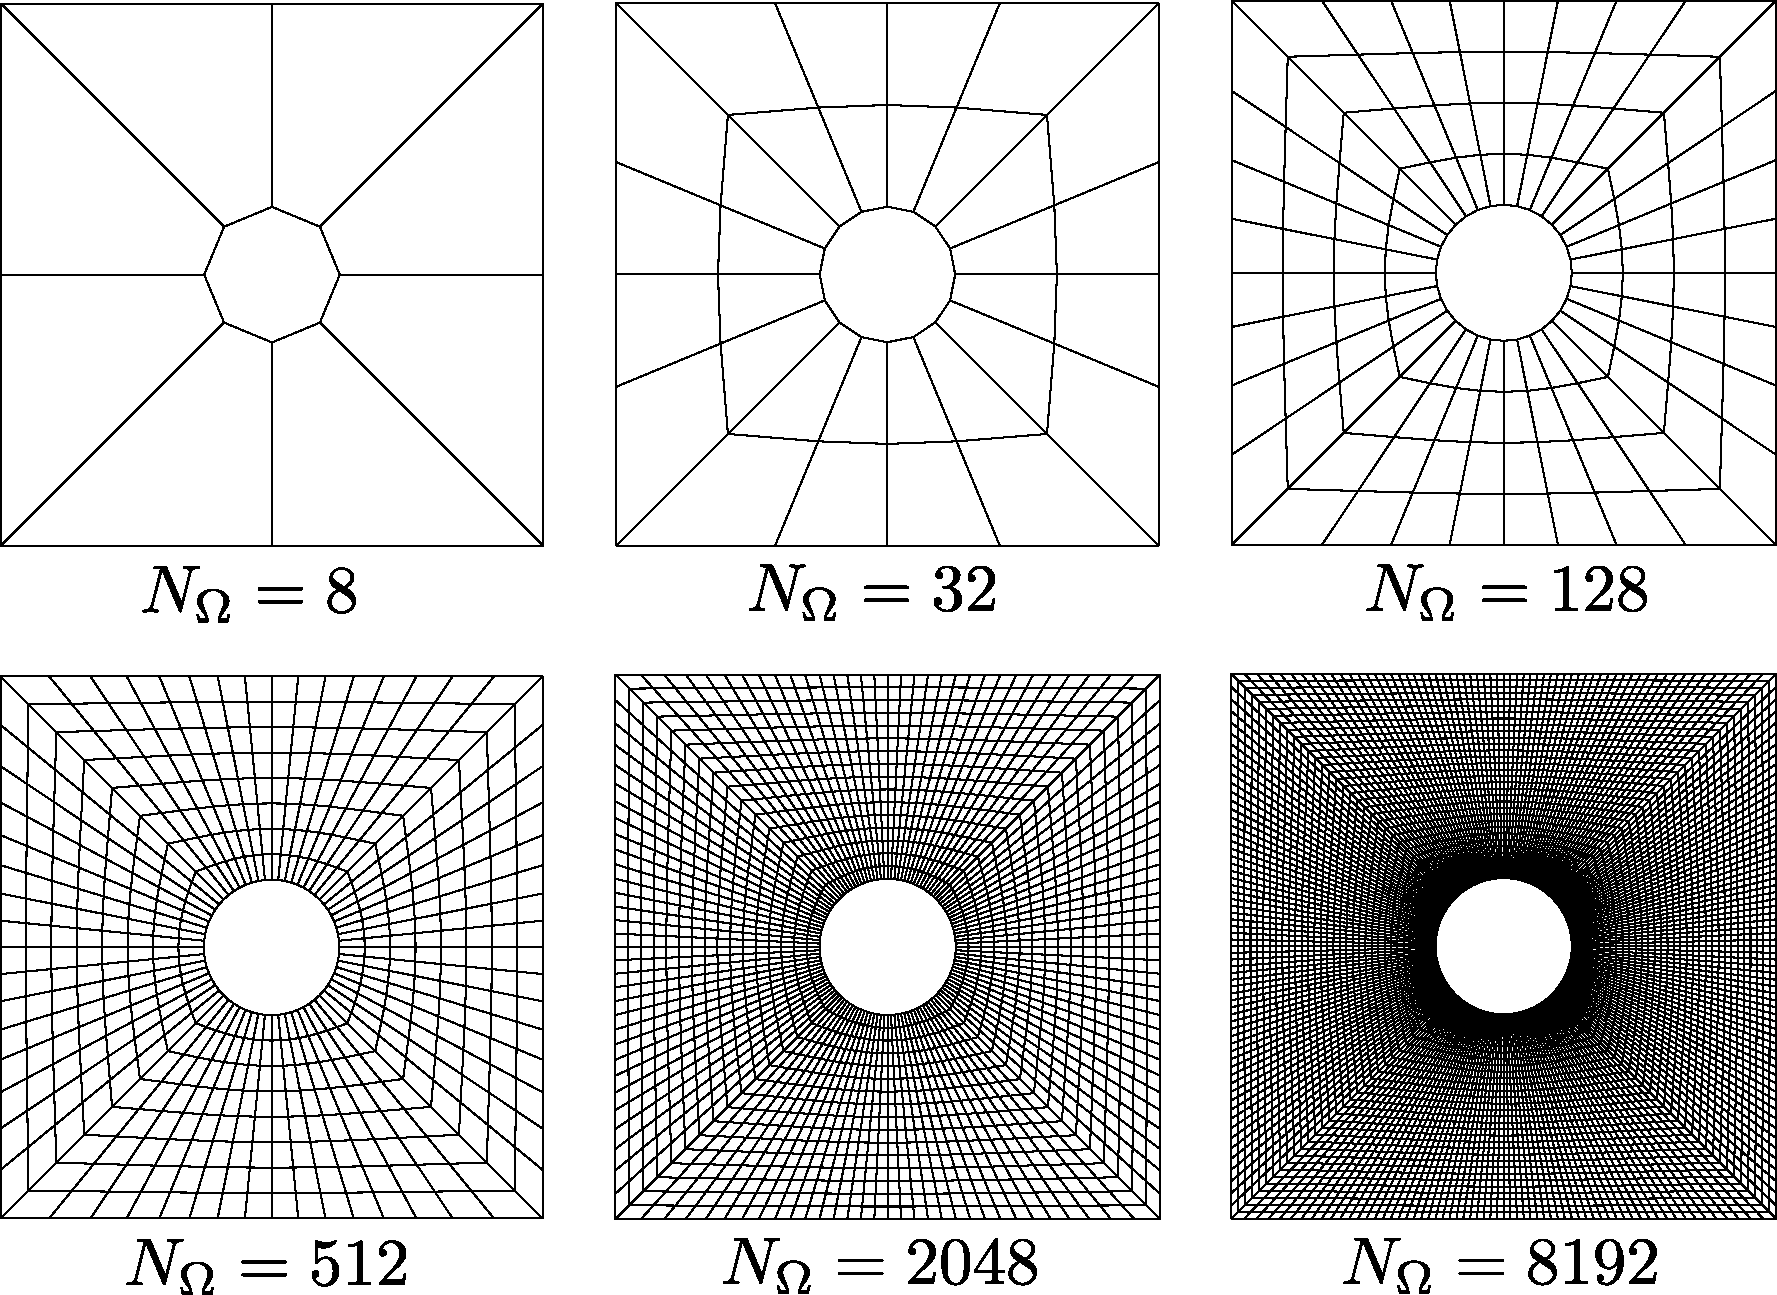
\includegraphics[width=6.0in]{figures/quad_hole_meshes.pdf}
  \caption{Quadrilateral meshes with varying levels of refinement.}
  \label{fig:plate_with_hole_meshes}
\end{figure}
A convergence study was carried out using a series of quadrilateral meshes with varying levels of refinement, discretizing the restricted problem domain $X_i \in [ -1, +1], \, \, i = 1, \, 2$ with $a = 0.25$ (see figure \ref{fig:plate_with_hole_meshes}.) The meshes consisted of either 4-node quadrilateral or 8-node serendipity quadrilateral elements. In each case, the elements employed either an isoparametric formulation, or a sufficiently high-order DG-PEM formulation (i.e. $k=1$ for 4-node quadrilaterals, and $k=2$ for 8-node quadrilaterals.) Displacement boundary conditions were prescribed to be consistent with the exact solution on the restricted domain boundary.

Displacement and stress error norms were computed with reference to the exact solution for the following problem parameters: $E = 29000.0$, $\nu = 0.3$, and $T = 1.0$. Convergence plots for the displacement and stress error norms are provided in Figures \ref{fig:plate_with_hole_l2_errors} and \ref{fig:plate_with_hole_h1_errors}, respectively.

\begin{figure}[!h]
  \centering
    \begin{subfigure}[b]{0.49\linewidth}
            \centering
            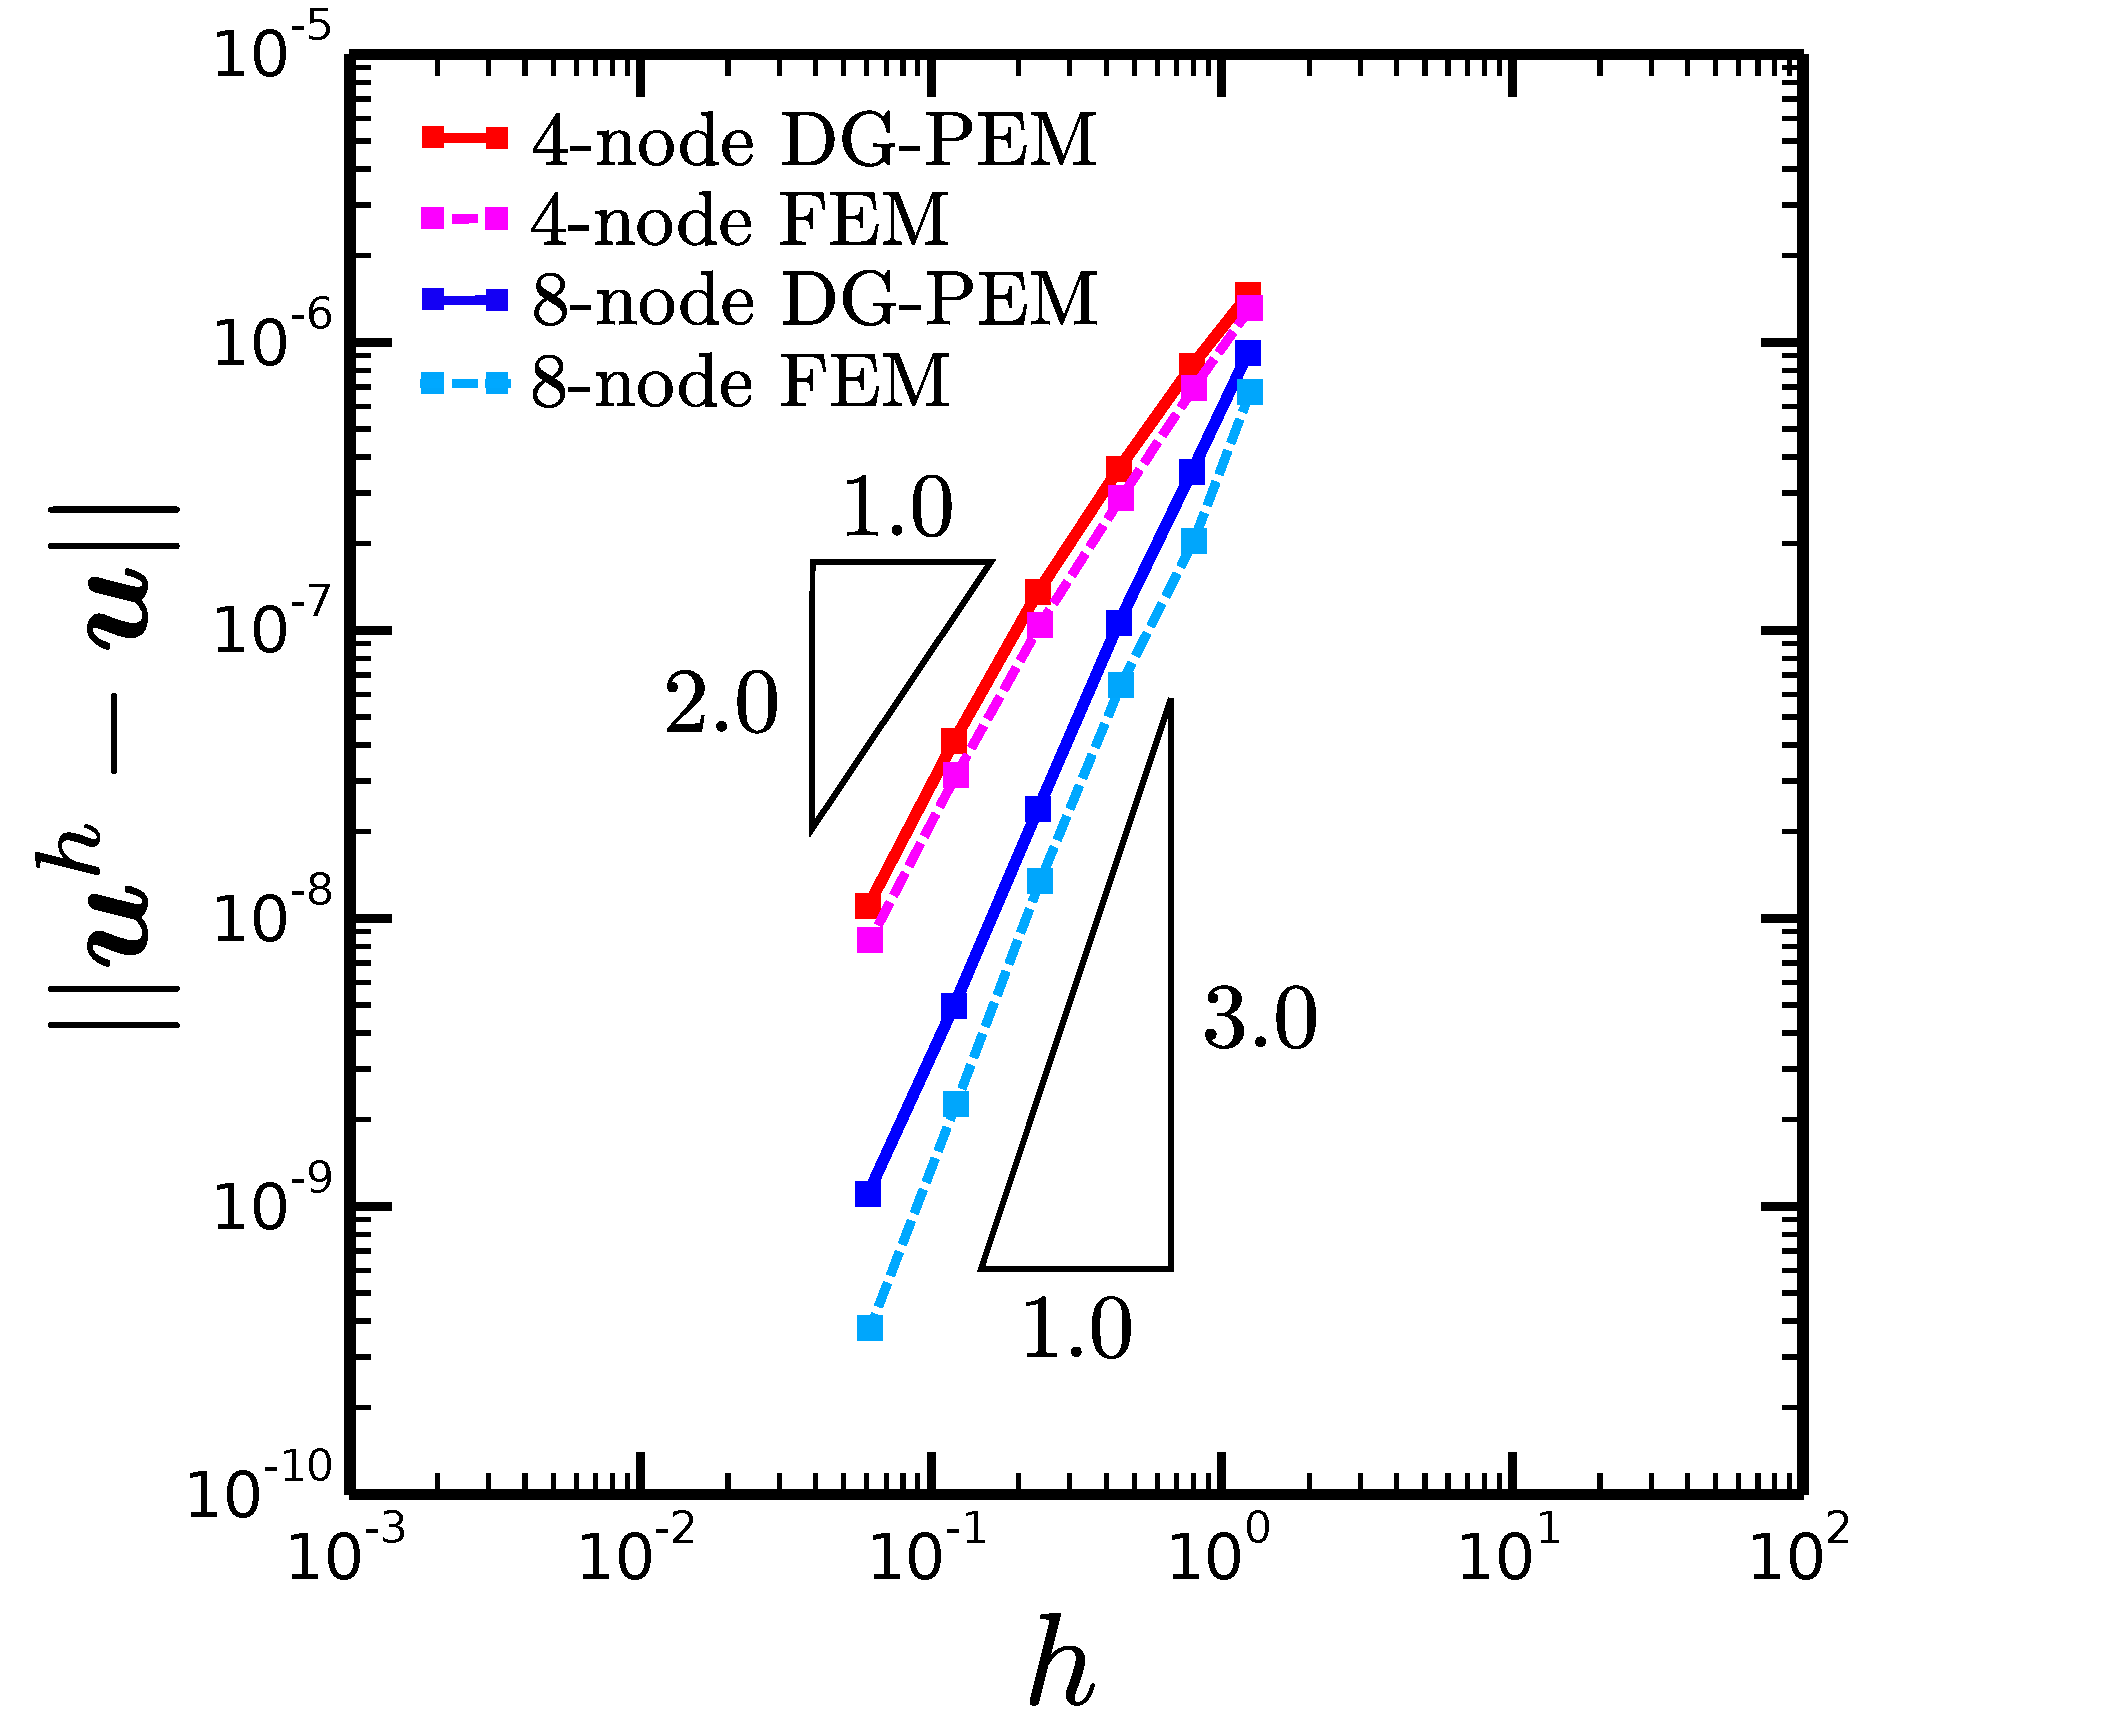
\includegraphics[width=3.3in]{figures/plate_with_hole_l2_errors.pdf}
    			\caption{displacement errors \label{fig:plate_with_hole_l2_errors}}
    \end{subfigure}
	\begin{subfigure}[b]{0.49\linewidth}
            \centering
            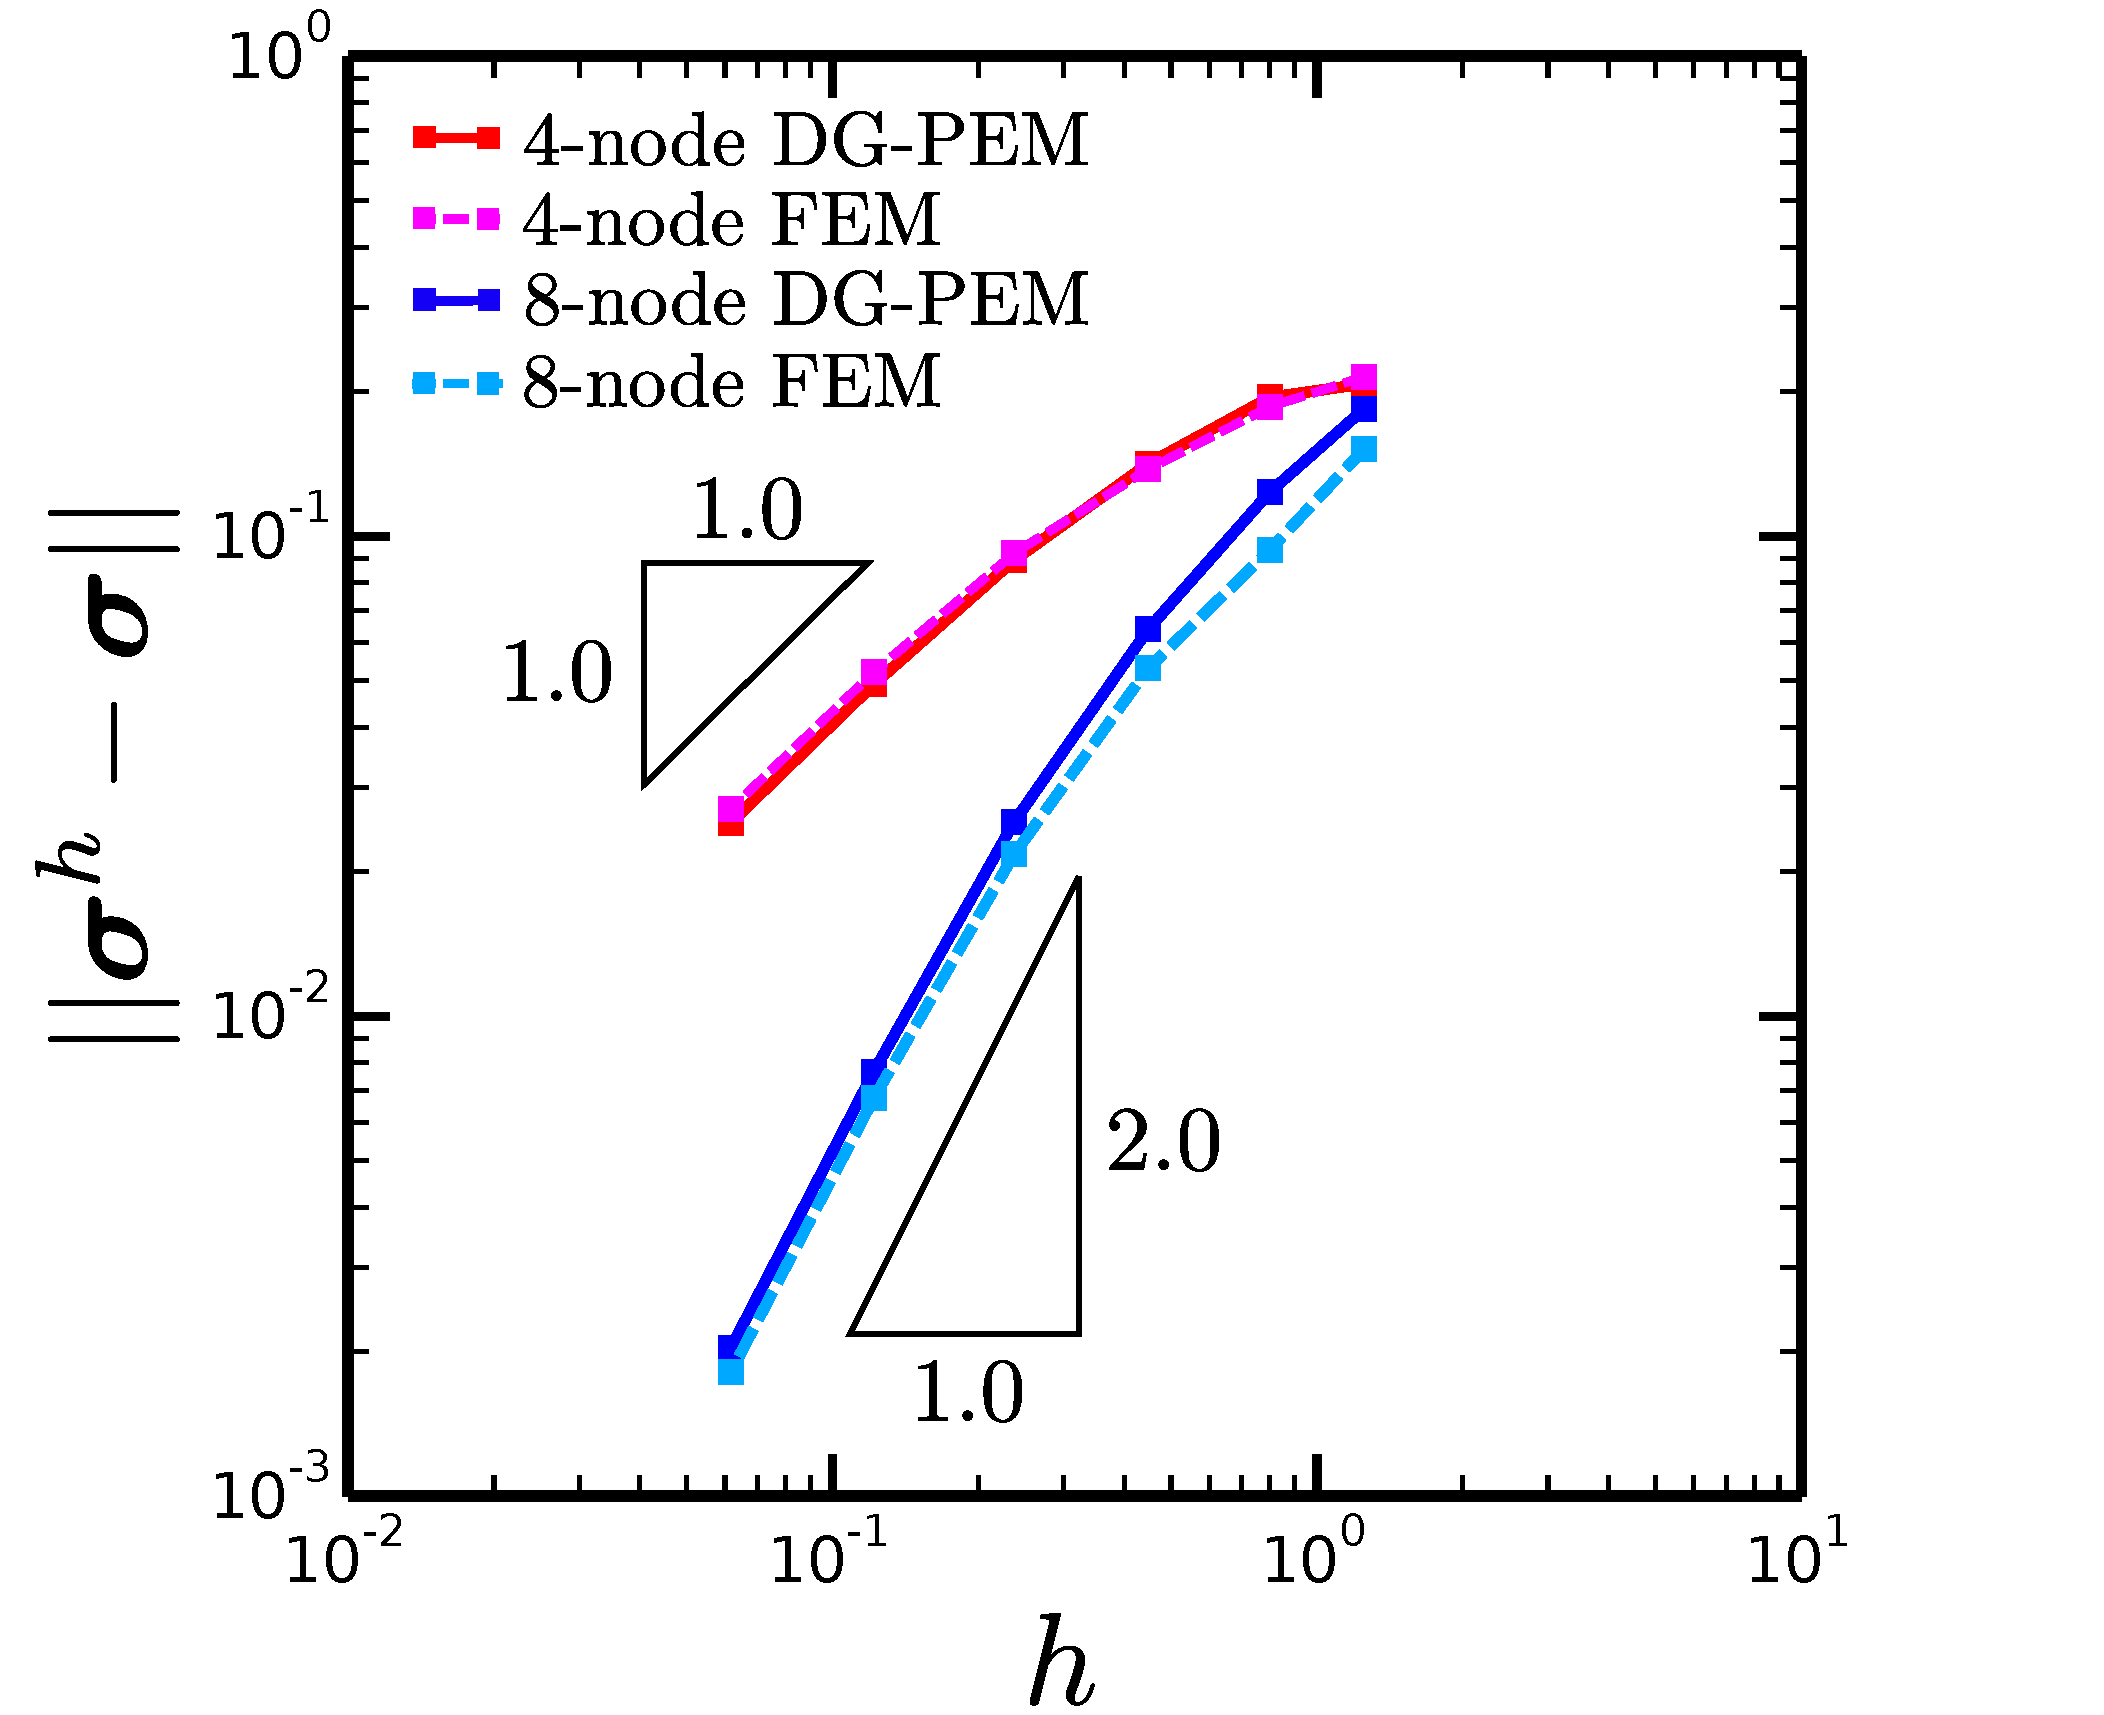
\includegraphics[width=3.3in]{figures/plate_with_hole_h1_errors.pdf}
    			\caption{stress errors \label{fig:plate_with_hole_h1_errors}}
    \end{subfigure} \caption{Convergence plots for the plate with hole problem using FEM and DG-PEM.}
  \label{fig:plate_with_hole_errors}
\end{figure}

For a given element formulation, the \textit{rate} of convergence in the two error metrics
\begin{equation}
	|| \mathbf{u}^h - \mathbf{u} || \leq C h^p || \mathbf{u} ||, \quad || \boldsymbol{\sigma}^h - \boldsymbol{\sigma} || \leq C h^q || \boldsymbol{\sigma} ||,
\end{equation}
is characterized by the powers $p$ and $q$, respectively. The average and maximal rates of convergence for each element formulation across all levels of mesh refinement are displayed in Table \ref{tab:plate_with_hole_convergence_rates}.

\begin{table}[!ht]
  \begin{center}
    \begin{tabular}{| l || c | c || c | c |}
    \hline
           & $p_{\text{avg}}$ & $p_{\text{max}}$ & $q_{\text{avg}}$ & $q_{\text{max}}$ \\ \hline \hline
    FEM (4-node quadrilateral)    & 1.66 (2.0) & 1.94 (2.0) & 0.66 (1.0) & 0.96 (1.0) \\ \hline
    DG-PEM (4-node quadrilateral) & 1.88 (2.0) & 2.13 (2.0) & 0.73 (1.0) & 0.99 (1.0) \\ \hline
    FEM (8-node quadrilateral)    & 2.48 (3.0) & 2.68 (3.0) & 1.43 (2.0) & 1.93 (2.0) \\ \hline
    DG-PEM (8-node quadrilateral) & 2.34 (3.0) & 3.02 (3.0) & 1.71 (2.0) & 2.42 (2.0) \\
    \hline
    \end{tabular}
    \caption{Average and maximal convergence rates for each method. The optimal rates are shown in parentheses.}
    \vspace{-5pt}
    \label{tab:plate_with_hole_convergence_rates}
    \vspace{-10pt}
  \end{center}
\end{table}

It should be noted that part of the solution error incurred for the coarse meshes may be attributable to the inexact representation of the problem geometry (the circular hole). This would explain why the observed convergence rates are lower at coarser levels of refinement, but approach the optimal rates as the mesh is further refined.

In the limit as $h \rightarrow 0$, the linear and quadratic DG-PEM converge at the optimal rates in both the displacement and stress error norms. Because the quadrilateral meshes in Figure \ref{fig:plate_with_hole_meshes} consist of non-affinely distorted elements, the FEM using 8-node serendipity elements does not achieve the optimal rates of convergence. Overall, the DG-PEM appears to converge at slightly faster rates than the FEM. However, the solution errors at coarser levels of refinement tend to be smaller for the FEM, in general.

Future work will seek to investigate the measured error and convergence rates of the PEM when the elements take on arbitrary shape, and for a variety of different formulations and penalization parameter settings.

\subsection*{Incompressible Twisting Annulus}

\begin{figure}[!h]
  \centering
  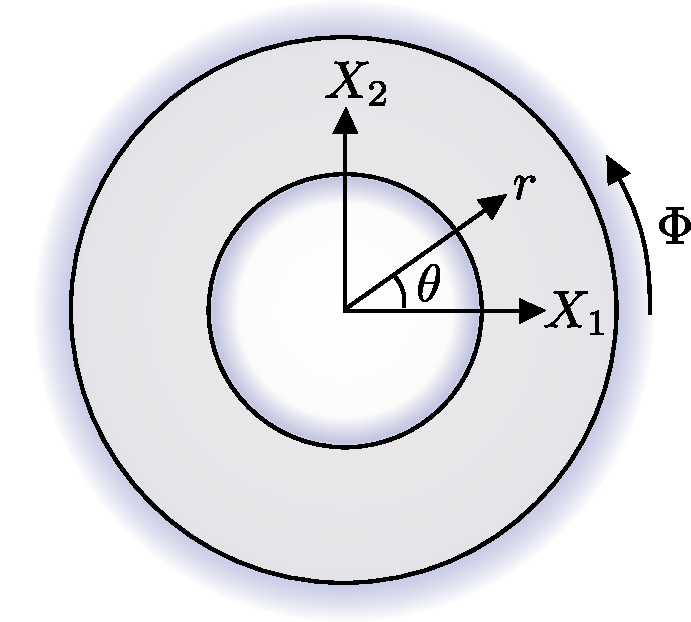
\includegraphics[width=3.0in]{figures/twisting_annulus_problem.pdf}  		\caption{Depiction of the twisting annulus problem.}
  \label{fig:twisting_annulus_problem}
\end{figure}
Consider the elastic annulus depicted in Figure \ref{fig:twisting_annulus_problem}, whose inner radius at $r = R_i$ is fixed, and whose outer radius $r = R_o$ rigidly rotates at an angular velocity of $\Phi$. The radially symmetric displacement boundary conditions for this motion are described by
\begin{equation}
	u_r (R_i,t) = u_r (R_o,t) = 0, \quad u_z (R_i,t) = u_z (R_o,t) = 0,
\end{equation}
\begin{equation}
	u_\theta (R_i,t) = 0, \quad u_\theta (R_o,t) = R_o \, \Phi \, t,
\end{equation}
for all $t \geq 0$.

Let the elastic material be characterized by the isotropic hypoelastic model of grade zero, consistent with the Jaumann rate of stress:
\begin{equation}
  \dot{\boldsymbol{\sigma}} = \mathbb{C} : \mathbf{D} + \mathbf{W} \boldsymbol{\sigma} - \boldsymbol{\sigma} \mathbf{W}.
\end{equation}
If the material is incompressible (if $\text{tr} (\mathbf{D}) = 0$), an analytical solution may be determined which is valid for finite deformations. The solutions for the displacement and stress fields are derived in the Appendix. The resulting expressions are given below:
\begin{equation}
  u_r = u_z = 0, \quad u_\theta = \frac{R_o^2}{r} \frac{r^2 - R_i^2}{R_o^{2} - R_i^{2}} \Phi t,
  	\label{eq:annulus_u_exact}
\end{equation}
\begin{equation}
  \sigma_{rr} = - \sigma_{\theta \theta} = \mu \frac{R_i^{2}}{r^{2}} \left[ \cos \left( 2 \frac{R_o^{2}}{R_o^{2} - R_i^{2}} \Phi t \right) - 1 \right], \quad \sigma_{r \theta} = \mu \frac{R_i^{2}}{r^{2}} \sin \left( 2 \frac{R_o^{2}}{R_o^{2} - R_i^{2}} \Phi t \right).
  	\label{eq:annulus_s_exact}
\end{equation}

Because the element formulations used herein possess only displacement degrees of freedom, it is not possible to run an analysis for a truly incompressible material. It suffices to examine numerical solutions in the near-incompressible regime (i.e. $\nu = 0.4999$). To combat the issue of volumetric locking, the kinematic enhancement suggested in \cite{Rashid:06} was implemented, and utilized in conjunction with each of the element formulations considered herein. Element formulations which have been ``enhanced'' in this manner are henceforth indicated as such.

Additionally, because an accurate prediction of the pressure field would otherwise require the use of a mixed formulation, the stress error metric in (\ref{eq:normalized_stress_error}) will be dominated by errors in the pressure field. For this reason, only the errors in the deviatoric stress field will be examined:
\begin{equation}
	\frac{||\mathbf{s}^h - \mathbf{s}||}{||\mathbf{s}||} = \sqrt{\frac{\int_{\mathcal{B}_0} (\mathbf{s}^h - \mathbf{s}) \colon (\mathbf{s}^h - \mathbf{s}) \, dV}{\int_{\mathcal{B}_0} \mathbf{s} \colon \mathbf{s} \, dV}},
	\label{eq:deviator_stress_error}
\end{equation}
where $s_{ij} = \sigma_{ij} - \frac{1}{3} \sigma_{kk} \delta_{ij}$ denotes the stress deviator.

\begin{figure}[!h]
  \centering
  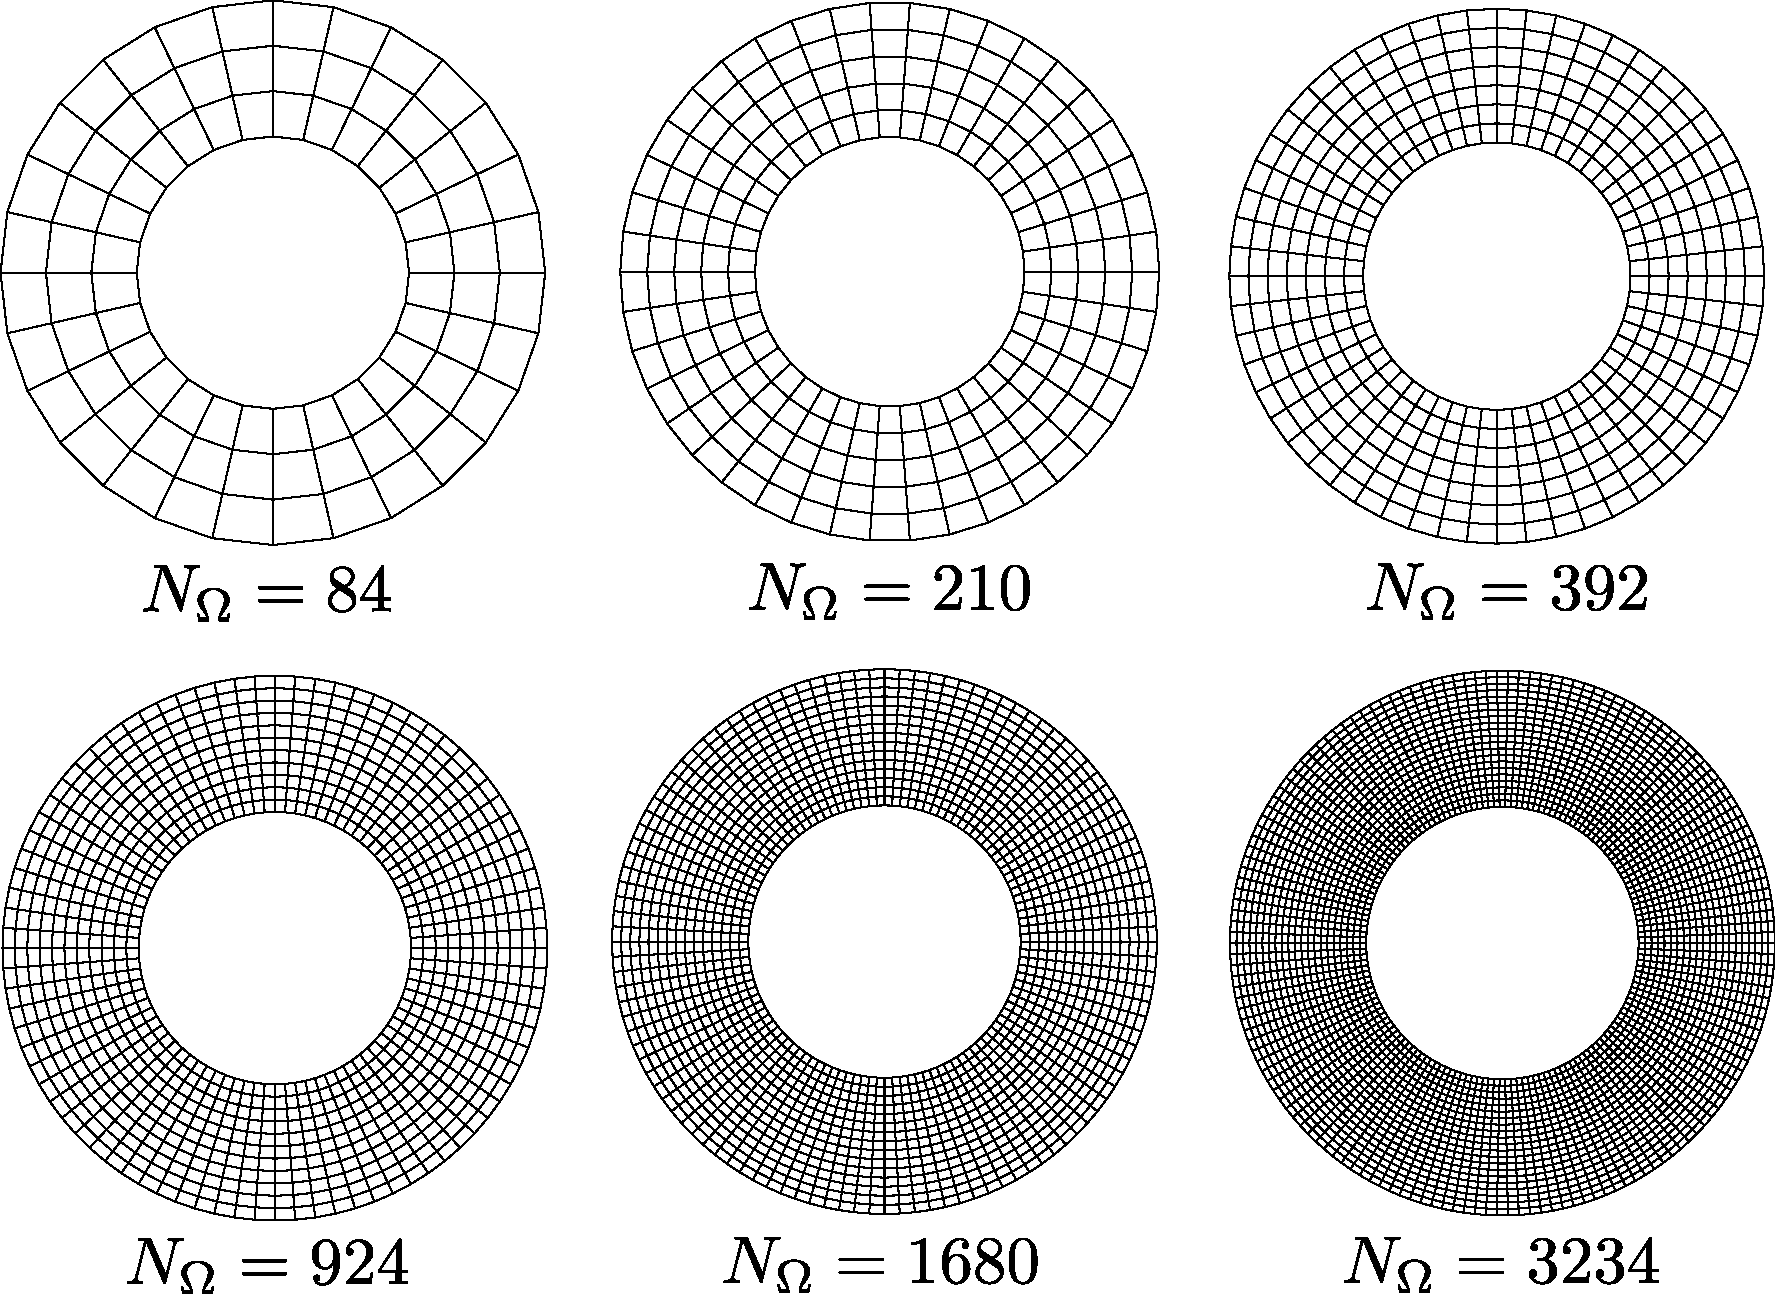
\includegraphics[width=5.0in]{figures/hex_annulus_meshes.pdf}
  \caption{Hexahedral meshes with varying levels of refinement for the twisting annulus problem.}
  \label{fig:hex_annulus_meshes}
\end{figure}

\begin{figure}[!h]
  \centering
  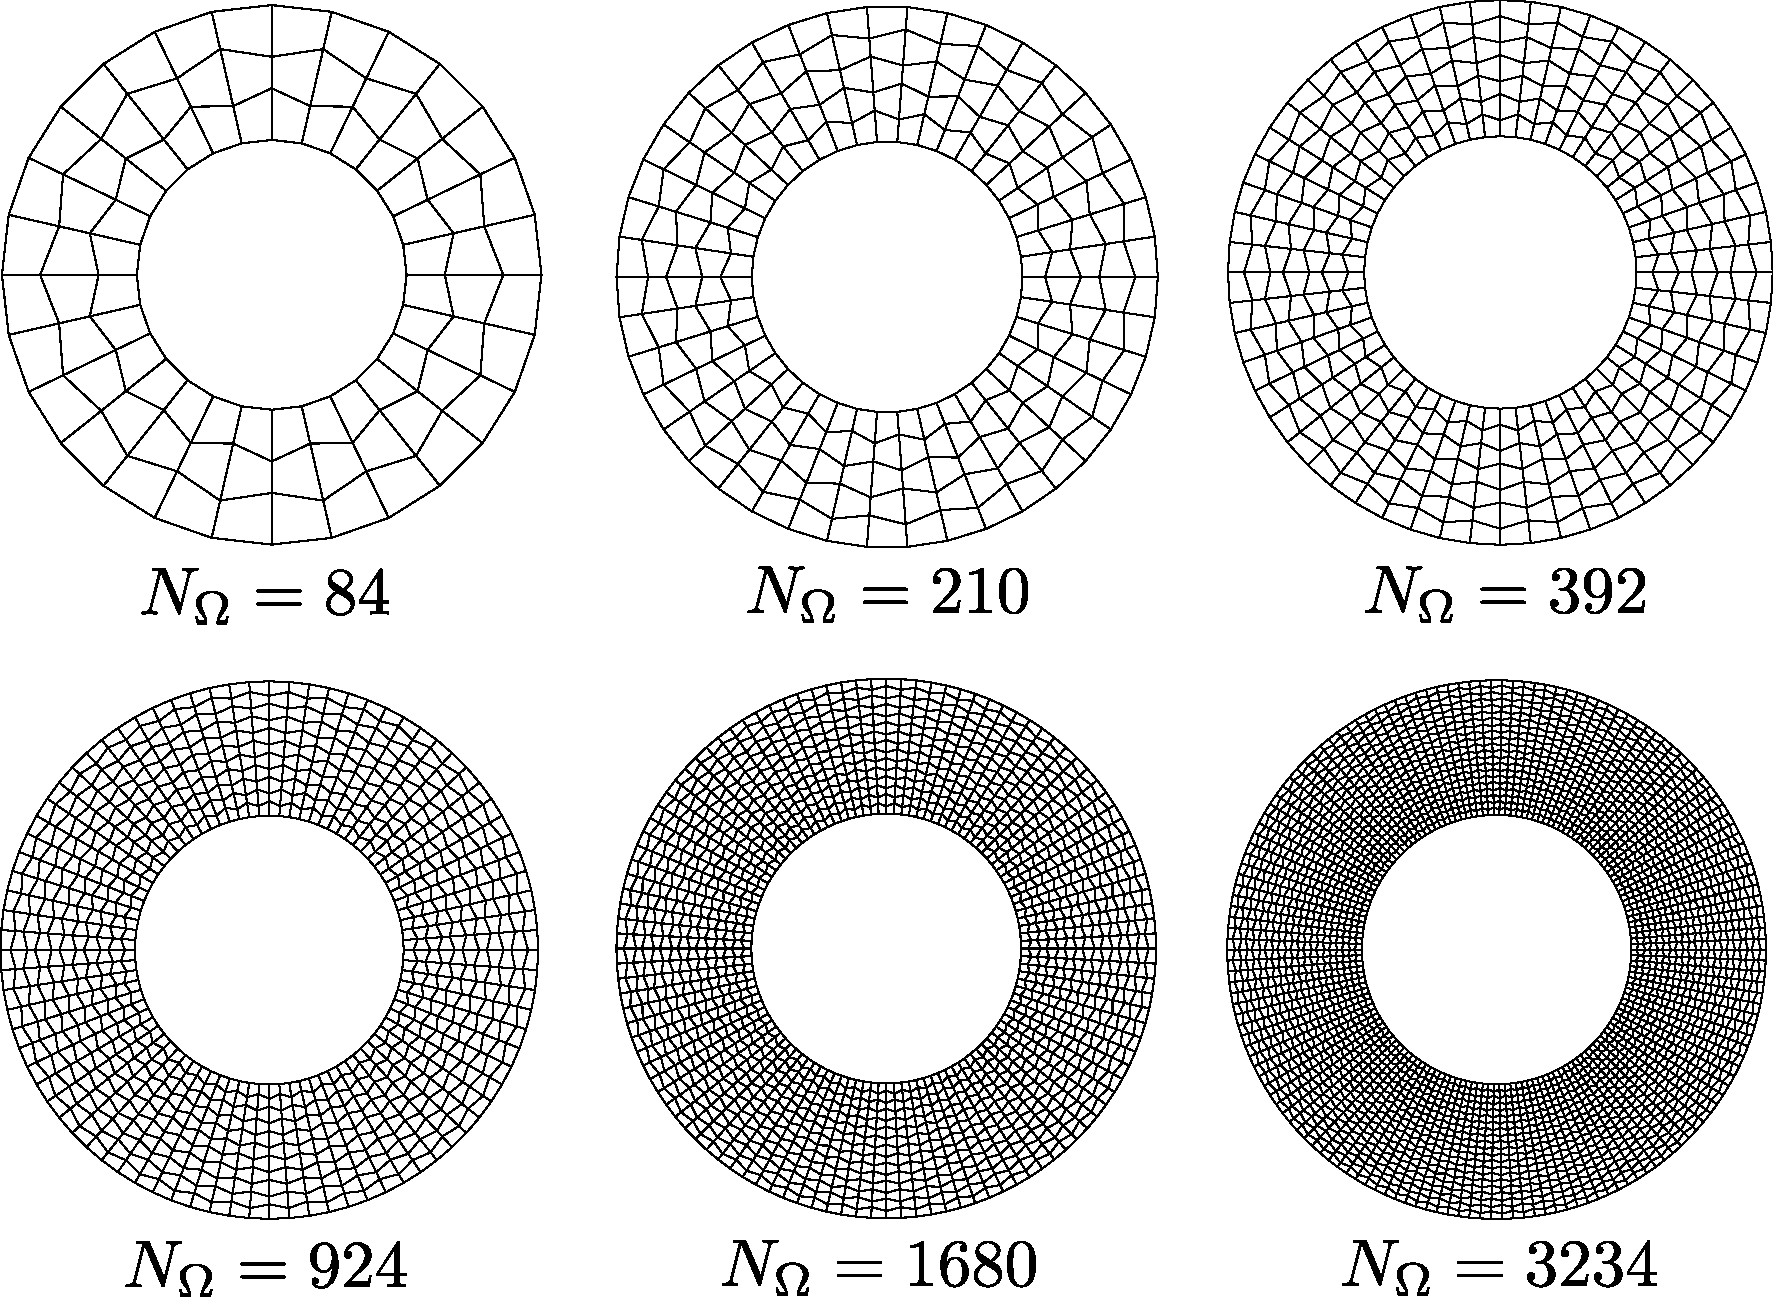
\includegraphics[width=5.0in]{figures/hexp_annulus_meshes.pdf}
  \caption{Distorted hexahedral meshes with varying levels of refinement for the twisting annulus problem.}
  \label{fig:hexp_annulus_meshes}
\end{figure}

\begin{figure}[!h]
  \centering
  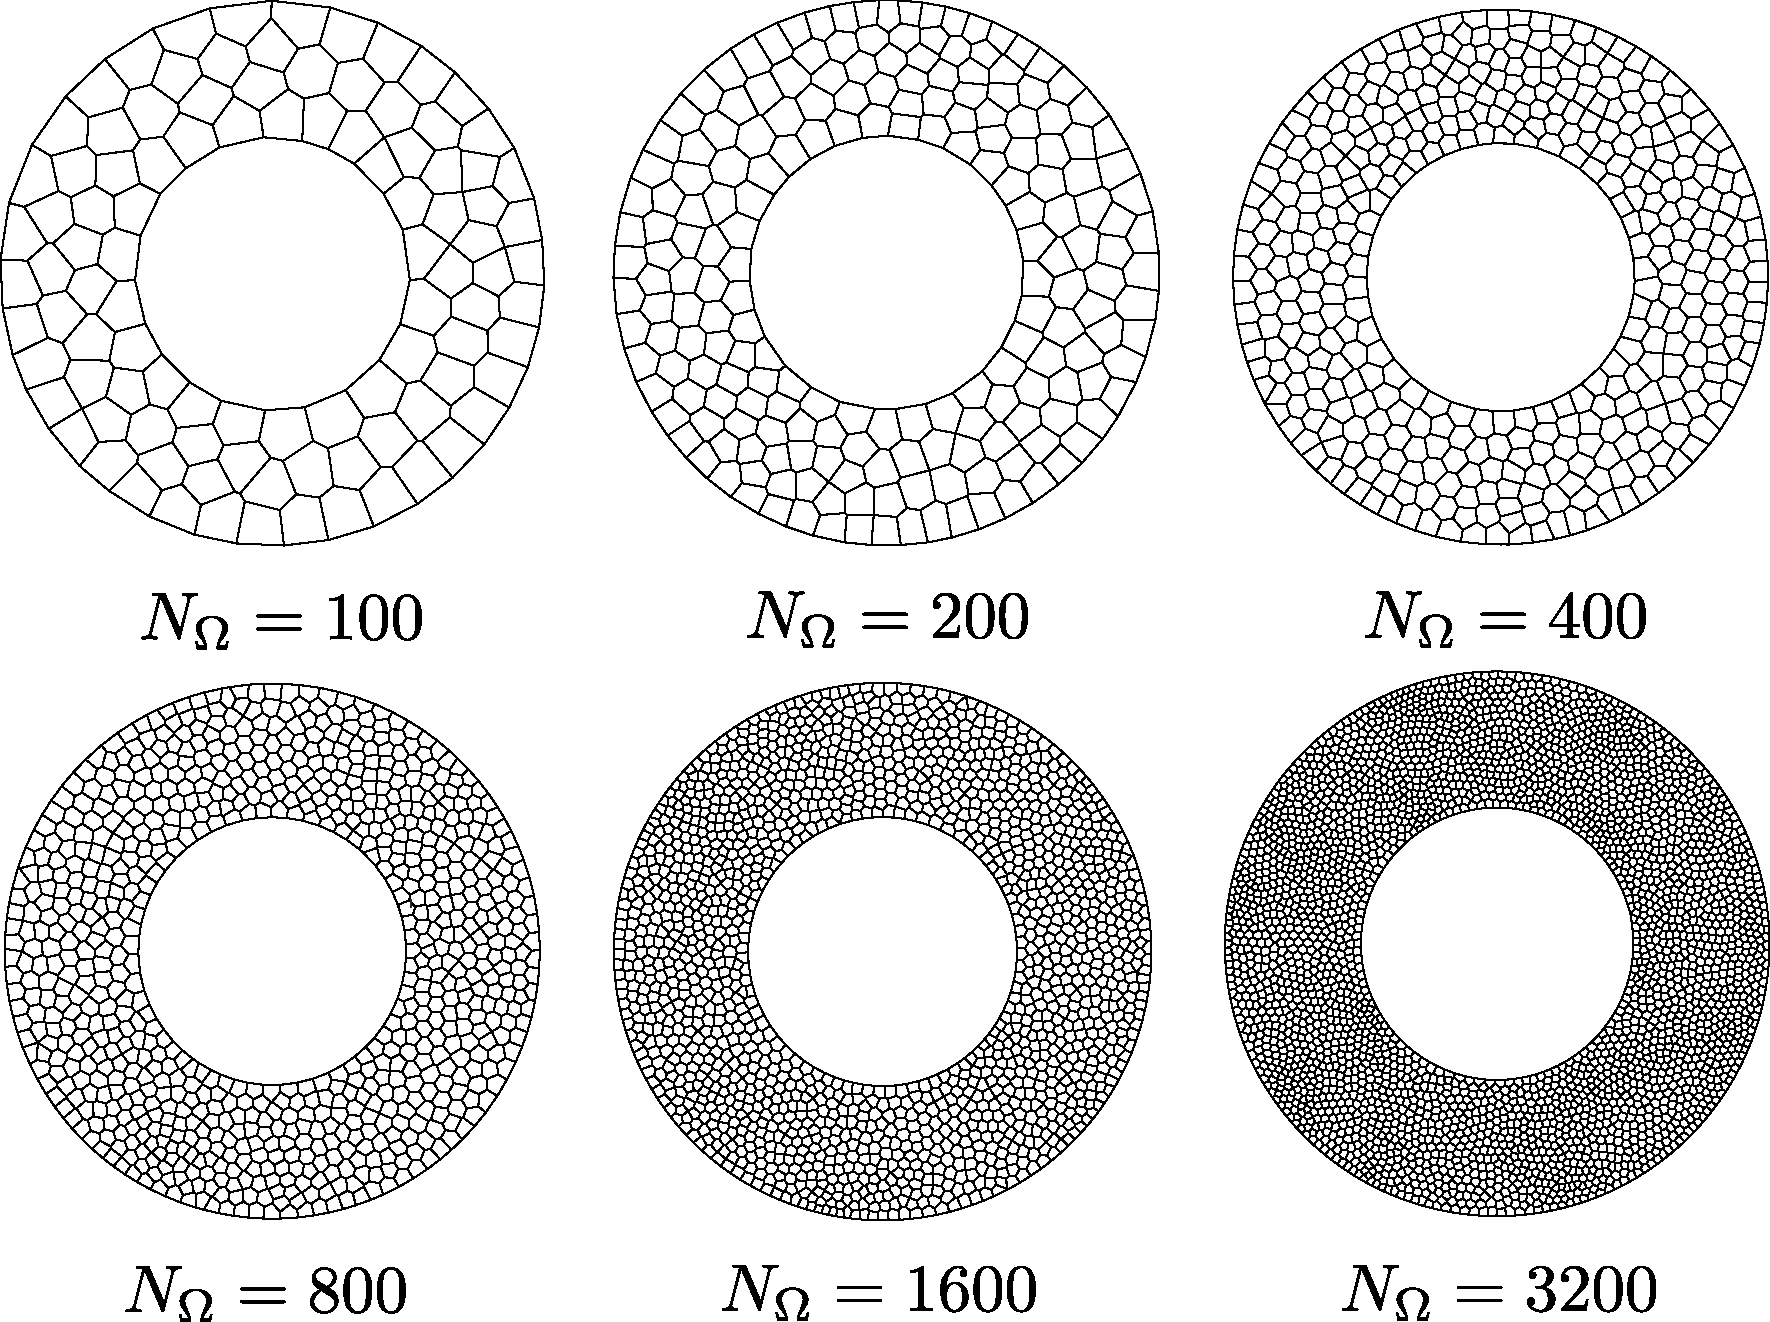
\includegraphics[width=5.0in]{figures/poly_annulus_meshes.pdf}
  \caption{Polyhedral meshes with varying levels of refinement for the twisting annulus problem.}
  \label{fig:poly_annulus_meshes}
\end{figure}

Convergence studies were carried out using the hexahedral and polyhedral meshes depicted in Figures \ref{fig:hex_annulus_meshes}, \ref{fig:hexp_annulus_meshes}, and \ref{fig:poly_annulus_meshes}. The hexahedral meshes were used in conjunction with the FEM, whereas the polyhedral meshes were used in conjunction with the DG-PEM. Each mesh consisted of a single layer of elements in the $z$-direction. All $z$-displacements were constrained, consistent with the assumptions of plane strain.

Finite deformations were considered in the analysis, albeit at relatively small strains (roughly 0.26\%). Error norms were computed with reference to the exact solution using the following problem parameters: $R_i = 0.5$, $R_o = 1.0$, $\Phi = 0.001$, $E = 1.0$, $\nu = 0.4999$, $t \in [0.0, \, 1.0]$.

For a given element formulation, the rate of convergence in the two error metrics
\begin{equation}
	|| \mathbf{u}^h - \mathbf{u} || \leq C h^p || \mathbf{u} ||, \quad || \mathbf{s}^h - \mathbf{s} || \leq C h^q || \mathbf{s} ||,
\end{equation}
is characterized by the powers $p$ and $q$, respectively. The average and maximal rates of convergence for each element type across all levels of mesh refinement are displayed in Table \ref{tab:twisting_annulus_convergence_rates}. A convergence plot is provided in Figure \ref{fig:twisting_annulus_errors} for the purposes of comparison.

%\begin{table}[!ht]
%  \begin{center}
%    \begin{tabular}{| c || c | c |}
%    \hline
%           & $q_{\text{avg}}$ & $q_{\text{max}}$ \\ \hline \hline
%    4-node FEM       & 1.13 (1.0) & 1.22 (1.0) \\ \hline
%    linear DG-PEM    & 1.02 (1.0) & 1.17 (1.0) \\ \hline
%    8-node FEM       & 2.34 (2.0) & 2.40 (2.0) \\ \hline
%    quadratic DG-PEM & 1.71 (2.0) & 2.42 (2.0) \\
%    \hline
%    \end{tabular}
%    \caption{Average and maximal convergence rates and for each method. The optimal rates are shown in parentheses.}
%    \vspace{-5pt}
%    \label{tab:twisting_annulus_convergence_rates}
%    \vspace{-10pt}
%  \end{center}
%\end{table}

\begin{table}[!ht]
  \begin{center}
    \begin{tabular}{| l || c | c || c | c |}
    \hline
           & $p_{\text{avg}}$ & $p_{\text{max}}$ & $q_{\text{avg}}$ & $q_{\text{max}}$ \\ \hline \hline
    Hexahedra (FEM)                & 1.61 (2.0) & 2.72 (2.0) & 1.01 (1.0) & 1.01 (1.0) \\ \hline
    Hexahedra (enhanced)           & 1.91 (2.0) & 2.66 (2.0) & 1.01 (1.0) & 1.01 (1.0) \\ \hline
    Distorted Hexahedra (FEM)      & -0.66 (2.0) & 0.57 (2.0) & -0.03 (1.0) & 0.35 (1.0) \\ \hline
    Distorted Hexahedra (enhanced) & 0.51 (2.0) & 0.66 (2.0) & 0.28 (1.0) & 0.39 (1.0) \\ \hline
    Polyhedra (DG-PEM)             & 0.23 (2.0) & 0.92 (2.0) & 0.67 (1.0) & 1.04 (1.0) \\ \hline
    Polyhedra (enhanced)           & 2.05 (2.0) & 2.74 (2.0) & 1.11 (1.0) & 1.20 (1.0) \\
    \hline
    \end{tabular}
    \caption{Average and maximal convergence rates for each element type/formulation. The optimal rates are shown in parentheses.}
    \vspace{-5pt}
    \label{tab:twisting_annulus_convergence_rates}
    \vspace{-10pt}
  \end{center}
\end{table}

\begin{figure}[!h]
  \centering
    \begin{subfigure}[b]{0.49\linewidth}
            \centering
            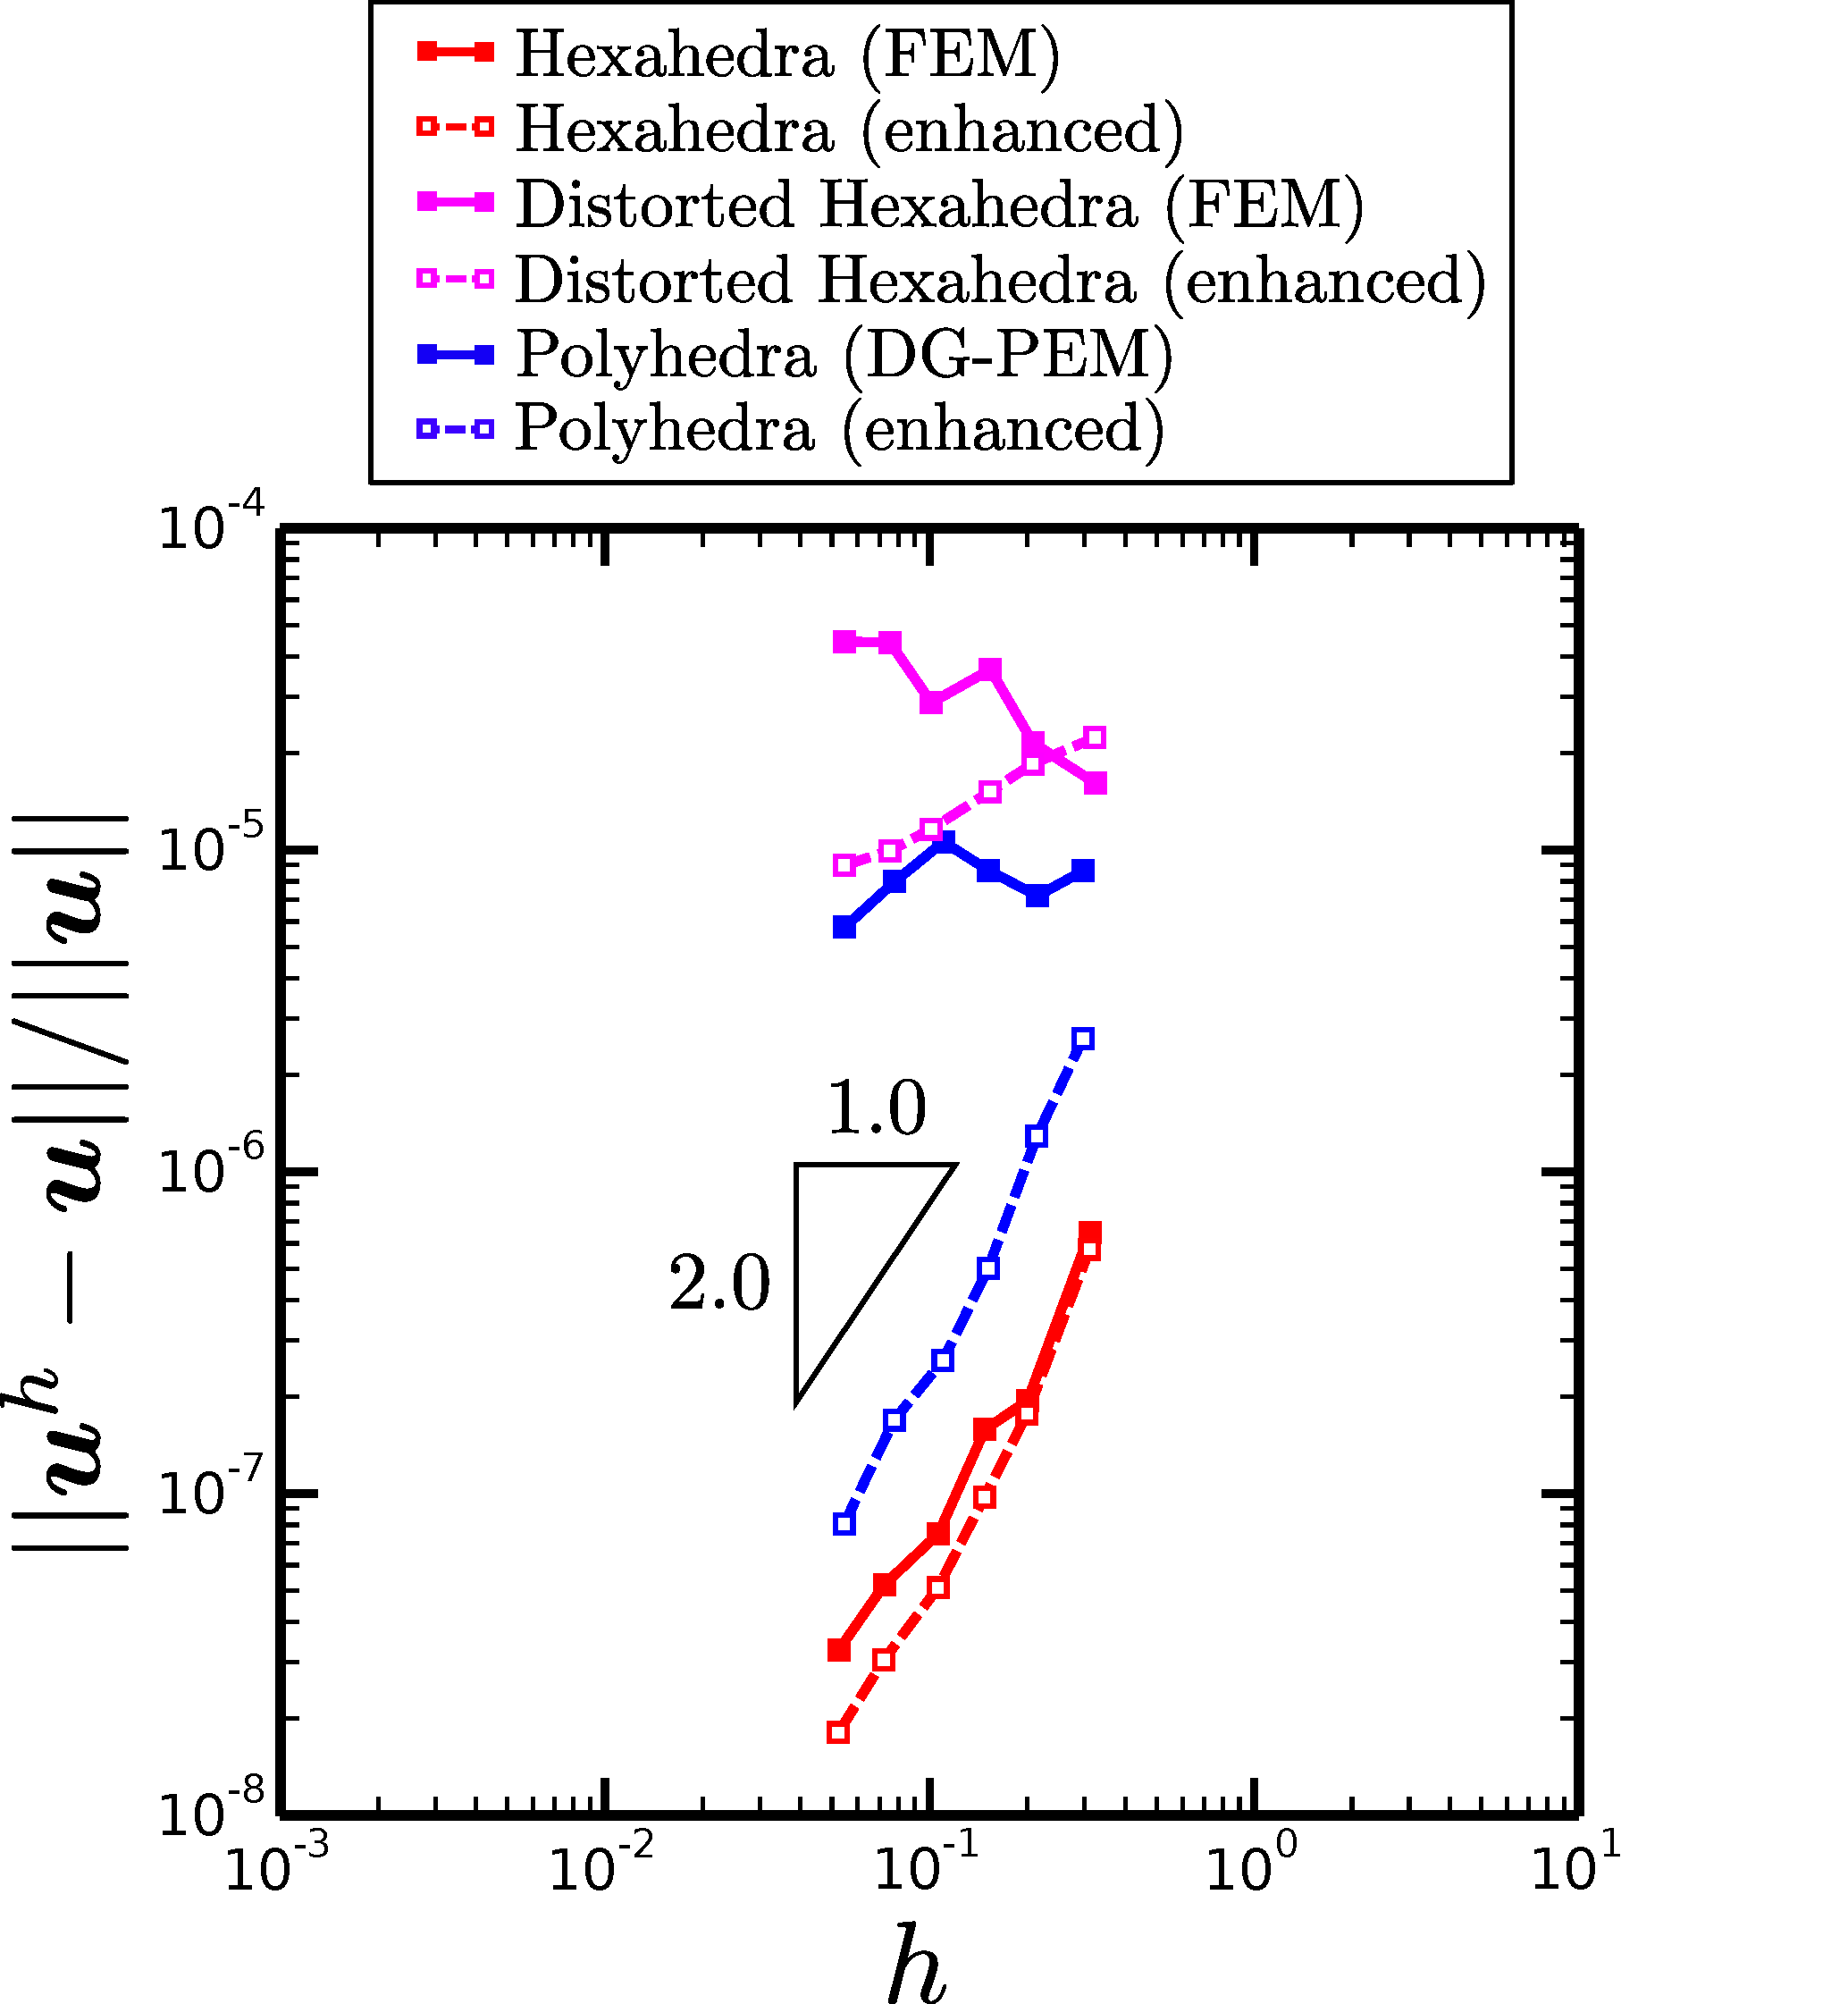
\includegraphics[width=3.3in]{figures/twisting_annulus_l2_errors.pdf}
    			\caption{displacement errors \label{fig:twisting_annulus_l2_errors}}
    \end{subfigure}
	\begin{subfigure}[b]{0.49\linewidth}
            \centering
            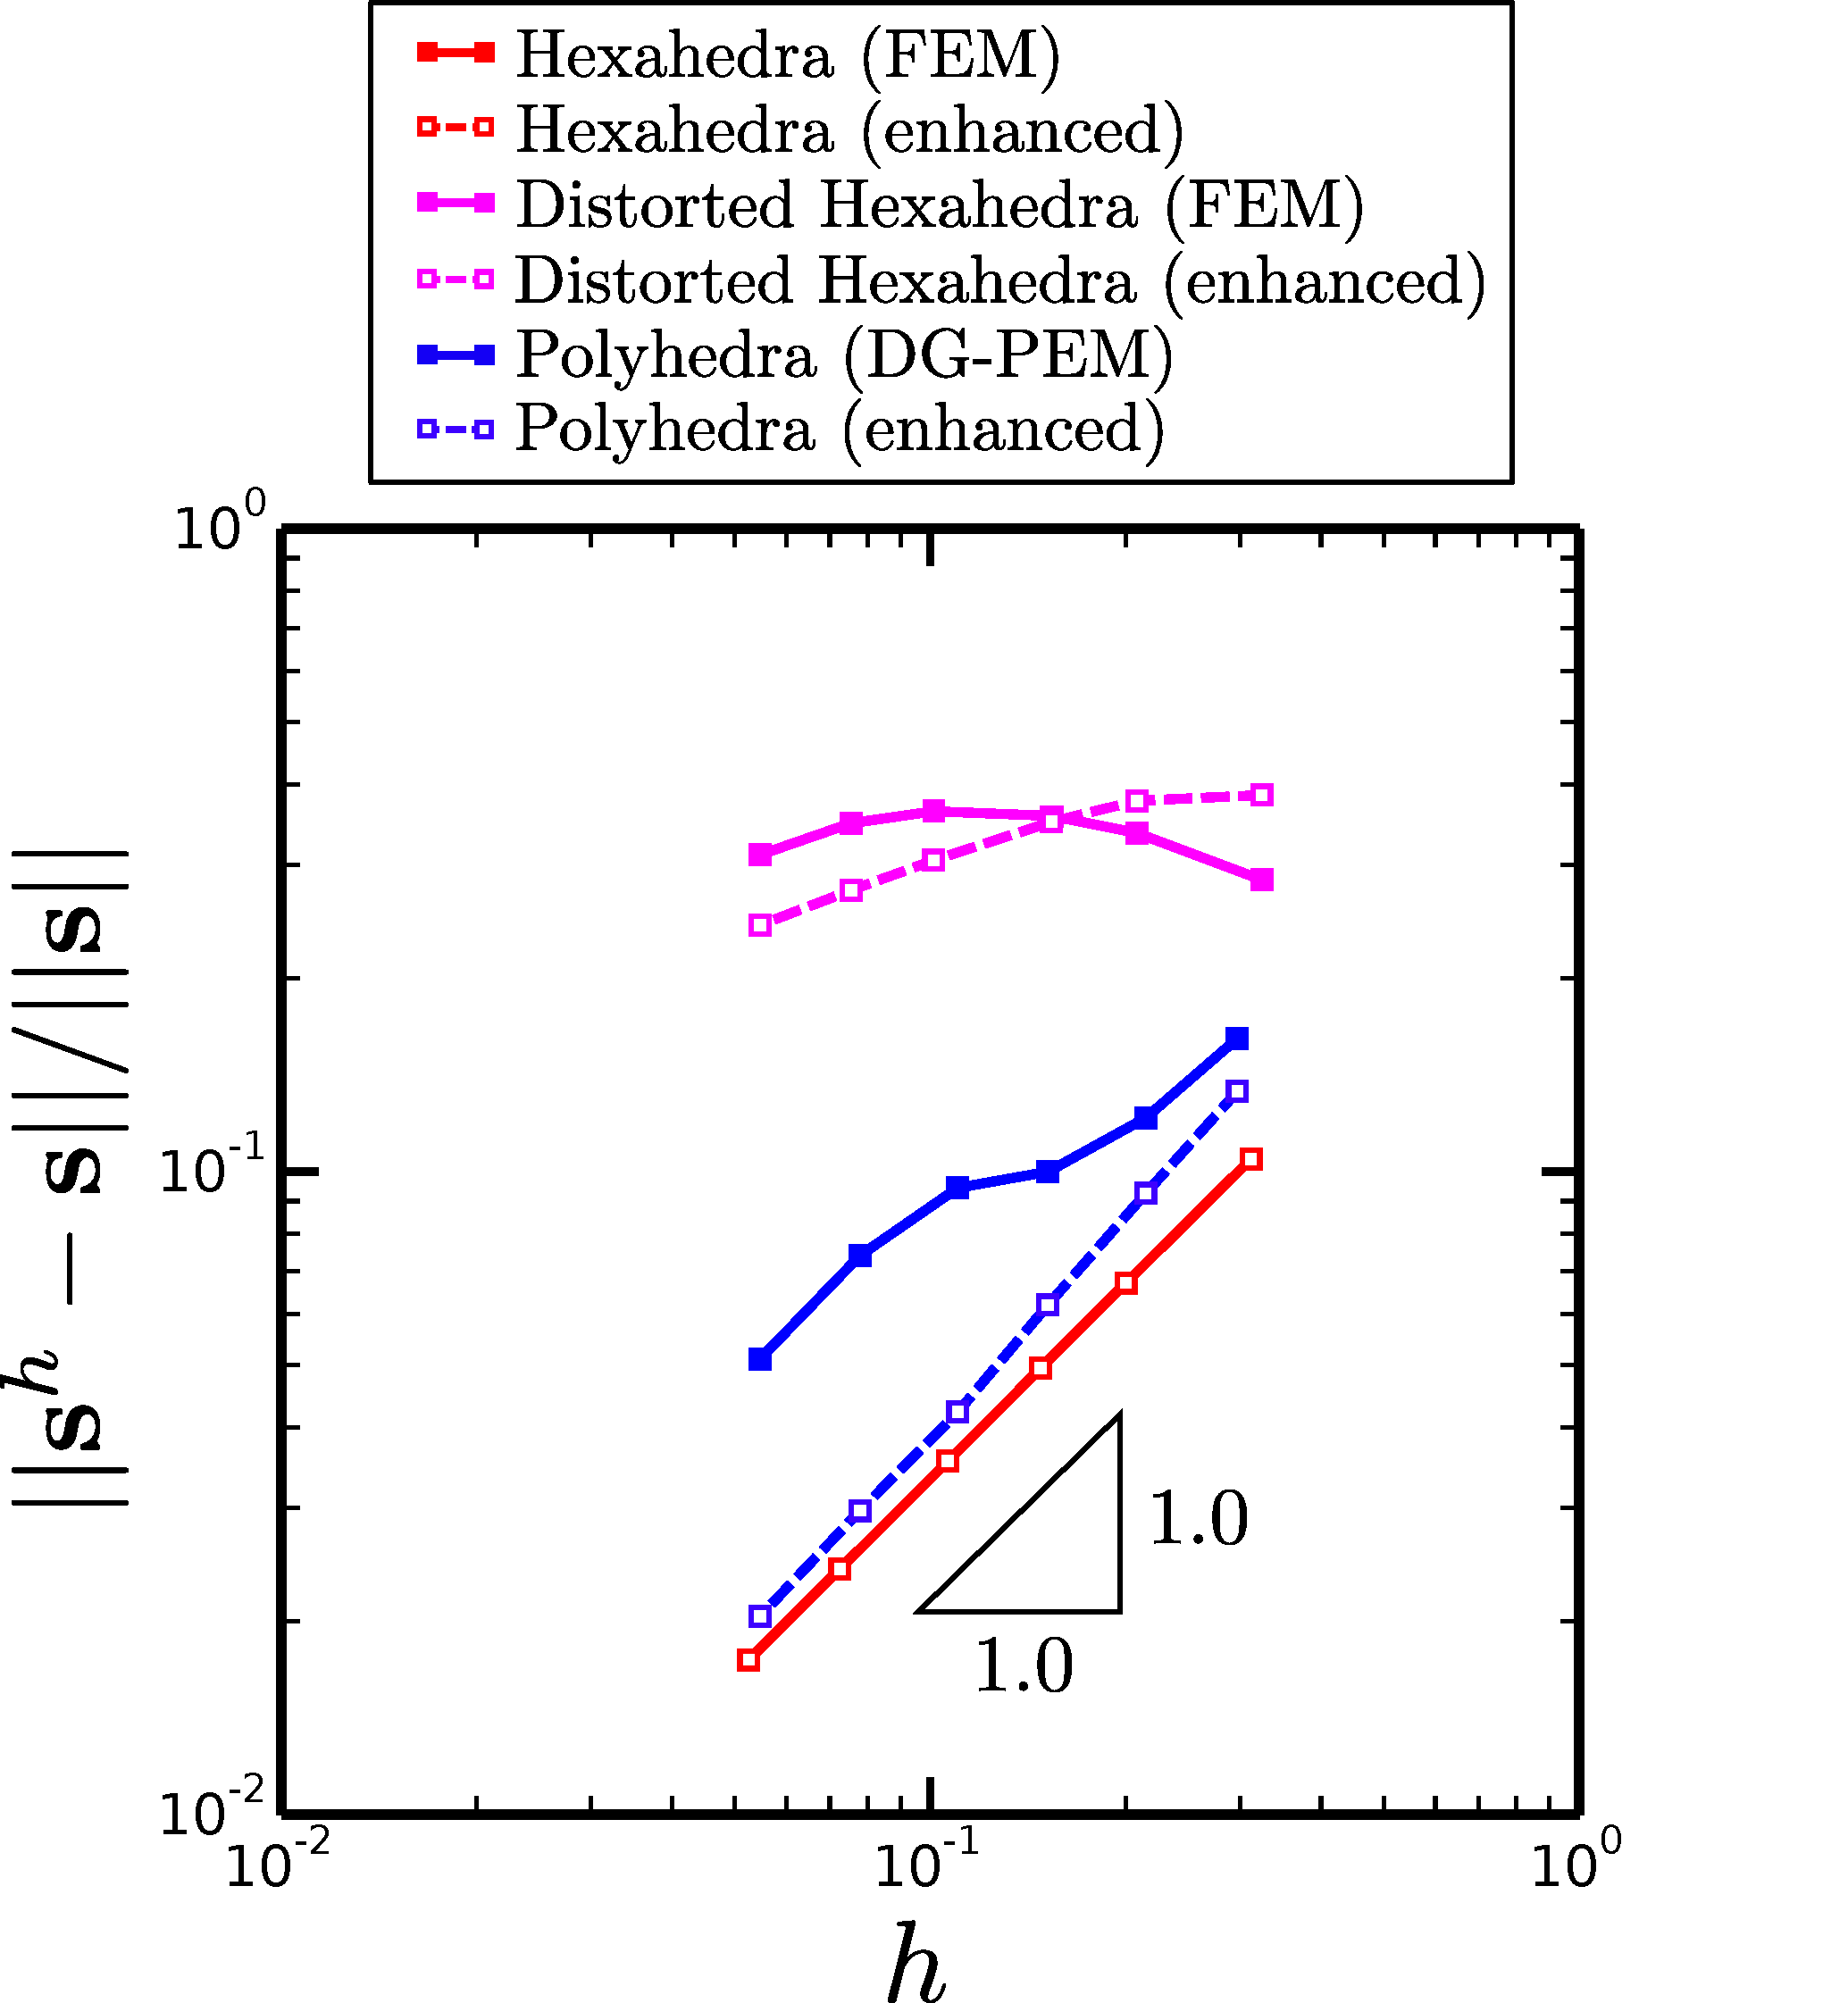
\includegraphics[width=3.3in]{figures/twisting_annulus_h1_errors.pdf}
    			\caption{stress deviator errors \label{fig:twisting_annulus_h1_errors}}
    \end{subfigure} \caption{Convergence plots for the twisting annulus problem using FEM for hexahedra and DG-PEM for polyhedra.}
  \label{fig:twisting_annulus_errors}
\end{figure}

Interestingly, the undistorted hexahedral meshes of Figure \ref{fig:hex_annulus_meshes} do not present symptoms of volumetric locking. On these meshes, both the standard and enhanced element formulations converge at roughly the same rates in the displacement and stress error norms.

In contrast, the distorted hexahedral meshes of Figure \ref{fig:hexp_annulus_meshes} succumb to spurious oscillations in the pressure field, regardless of whether the kinematic enhancement of \cite{Rashid:06} is employed. Figures \ref{fig:hexp_pressure} and \ref{fig:hexp_fbar_pressure} illustrate the characteristic ``checkerboard'' pattern in the pressure field that arises for the distorted meshes. The corresponding rates of convergence are only slightly improved for the enhanced formulation.

\begin{figure}[!h]
  \centering
    \begin{subfigure}[b]{0.32\linewidth}
            \centering
            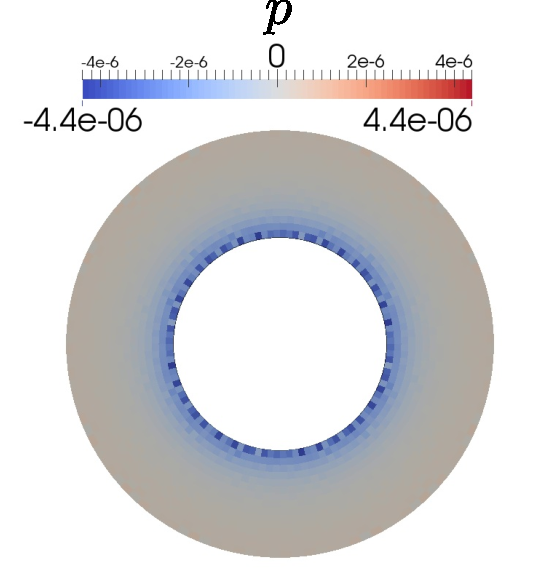
\includegraphics[width=2.1in]{figures/hex_pressure.pdf}
    			\caption{Hexahedra \label{fig:hex_pressure}}
    \end{subfigure}
	\begin{subfigure}[b]{0.32\linewidth}
            \centering
            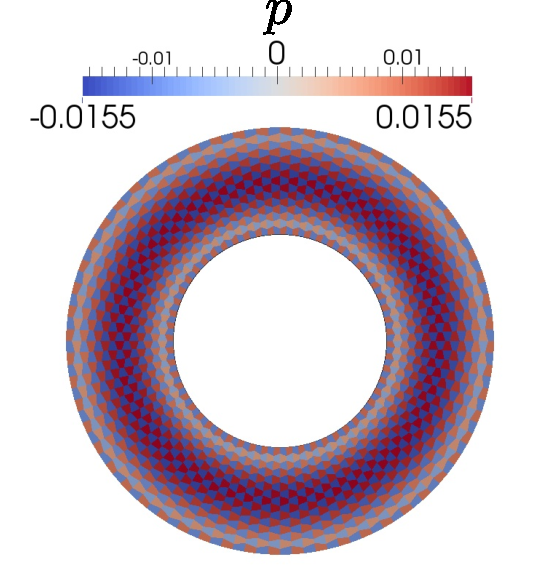
\includegraphics[width=2.1in]{figures/hexp_pressure.pdf}
    			\caption{Distorted \label{fig:hexp_pressure}}
    \end{subfigure} 
    \begin{subfigure}[b]{0.32\linewidth}
            \centering
            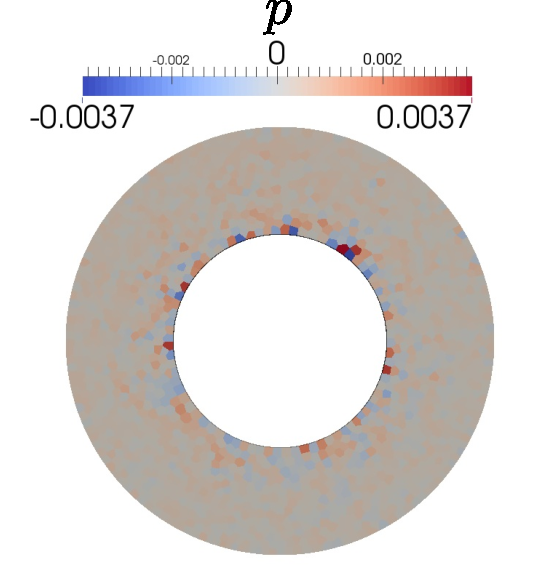
\includegraphics[width=2.1in]{figures/poly_pressure.pdf}
    			\caption{Polyhedra \label{fig:poly_pressure}}
    \end{subfigure}
    \begin{subfigure}[b]{0.32\linewidth}
            \centering
            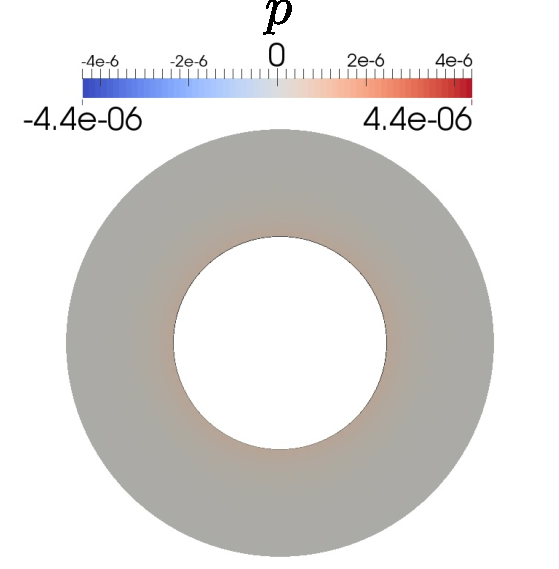
\includegraphics[width=2.1in]{figures/hex_fbar_pressure.pdf}
    			\caption{Hexahedra (enhanced) \label{fig:hex_fbar_pressure}}
    \end{subfigure}
	\begin{subfigure}[b]{0.32\linewidth}
            \centering
            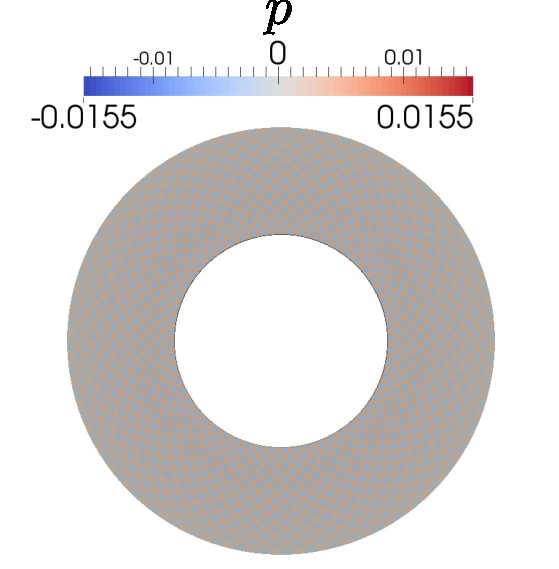
\includegraphics[width=2.1in]{figures/hexp_fbar_pressure.pdf}
    			\caption{Distorted (enhanced) \label{fig:hexp_fbar_pressure}}
    \end{subfigure} 
    \begin{subfigure}[b]{0.32\linewidth}
            \centering
            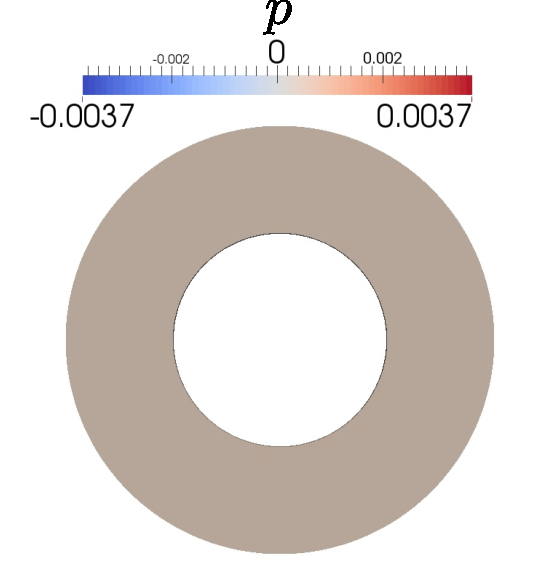
\includegraphics[width=2.1in]{figures/poly_fbar_pressure.pdf}
    			\caption{Polyhedra (enhanced) \label{fig:poly_fbar_pressure}}
    \end{subfigure} 
    \caption{Comparison of pressure fields for various element types and formulations. Color scales are kept consistent between similar mesh types.}
  \label{fig:twisting_annulus_stresses}
\end{figure}

The arbitrary polyhedral meshes of Figure \ref{fig:poly_annulus_meshes} are less sensitive to the effects of volumetric locking. Optimal rates of convergence are fully restored when the kinematic enhancement is utilized.

If the DG-PEM is utilized on either of the two series of hexahedral meshes shown in Figures \ref{fig:hex_annulus_meshes} and \ref{fig:hexp_annulus_meshes}, the resulting convergence rates match those of the FEM. This illustrates an important point: the particular choice of \textit{discretization} (the shape of the elements) controls mesh sensitivity to volumetric locking, more so than the underlying element formulation. Consider the extreme case of a mesh consisting entirely of linear tetrahedra. Such a mesh will produce identical results for the FEM, and all variants of the PEM. In the aforementioned scenario, volumetric locking will persist, regardless of which element formulation is utilized. The same rationale is true for the distorted hexahedral meshes. As such, the PEM should not be viewed as a direct remedy to volumetric locking. Rather, the PEM simply enables the use of more general discretizations, which may themselves be less suceptible to locking.

These observations lead to a related line of inquiry: can a given discretization be designed in such a fashion as to obviate locking altogether? Do random Voronoi meshes produce ``better'' results (in some statistical sense) over hexahedral meshes, and can such improvements be adequately quantified? With the geometric flexibility of the PEM in hand, the answers to these questions are within reach. The continued pursuit of such questions remains the subject of ongoing work.

%\subsection*{Thin Corner-Supported Plate}
%
%Consider a thin plate 
%(Description of the corner-supported plate problem).
%
%\begin{figure}[!h]
%  \centering
%  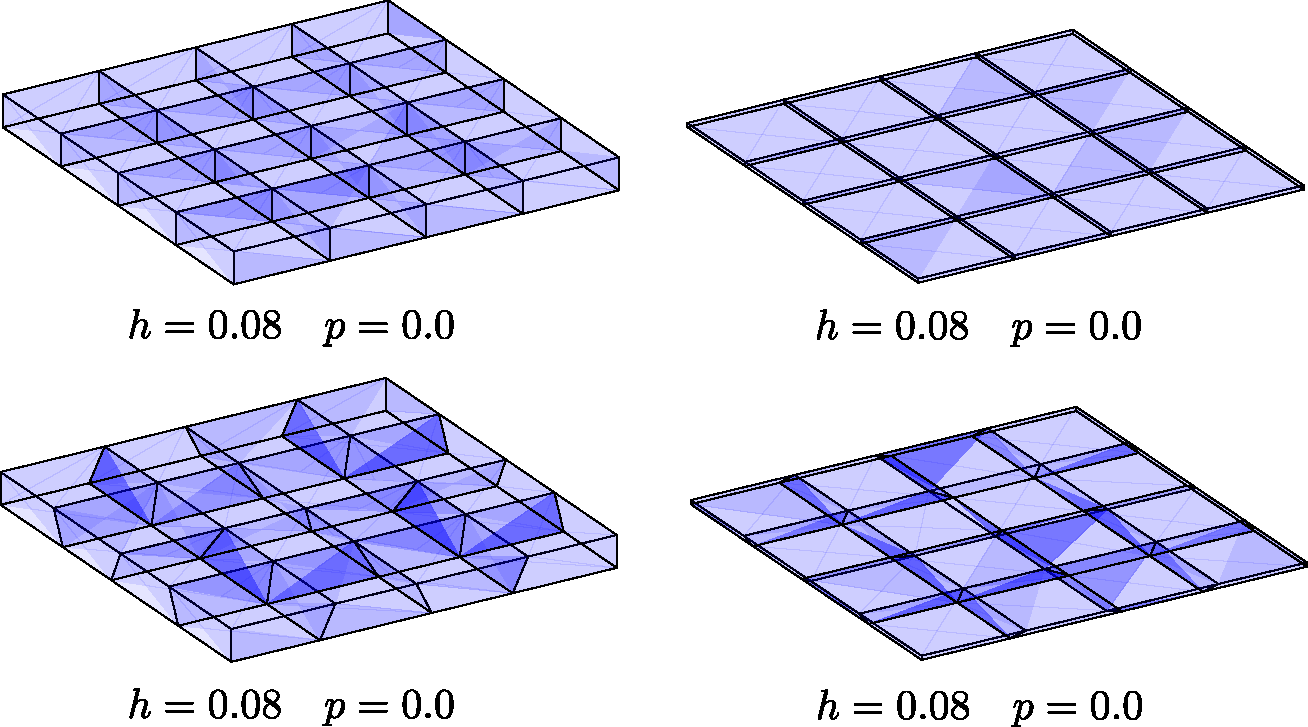
\includegraphics[width=6.0in]{figures/plate_meshes.pdf}
%  \caption{Hexahedral meshes with variable plate thickness $h$ and mesh perturbations $p$ for the corner-supported plate problem.}
%  \label{fig:plate_meshes}
%\end{figure}
%
%\subsubsection{Exact Solution}
%
%An exact solution for the vertical displacement field of the plate prob

%\section{Computational Efficiency}

%\subsection{Performance Comparison}

\section{Large Deformation Problems with Elasto-plastic Material Behavior}

A set of examples were explored to examine the behavior of the DG-PEM in the context of both geometric and material nonlinearity. The primary motivation for the present study is to evaluate the DG-PEM's ability to handle problems involving high plastic flow. Such problems pose two primary, yet opposing challenges: excessive plastic deformation may lead to mesh tangling and element inversion, and certain element types may succumb to volumetric locking, thereby preventing plastic deformation from occurring. To combat the latter problem, the kinematic enhancement suggested in \cite{Rashid:06} is utilized in conjunction with the element formulations considered herein. Unless noted otherwise, the DG-PEM employed the standard parameter settings utilized in previous problems.

A simple $J_2$ model for hypo-elasto-plasticity with linear isotropic hardening was implemented, employing the canonical radial return algorithm discussed in \cite{LSDYNA}. This model is utilized in the two problems considered in this section, entailing the specification of the following material parameters: Young's modulus $E$, Poisson's ratio $\nu$, an initial yield stress $Y_0$, and a linear hardening modulus $E_h$.

\subsection*{Necking of a Ductile Steel Tensile Specimen}

A tensile test for a 4130 steel plate specimen with square cross-section was simulated under isothermal conditions. The test setup was based in part upon the experimental procedures discussed in \cite{Gerberich:62}. The dimensions of the plate specimen illustrated in Figure \ref{fig:tensile_specimen_dimensions} conform with the ASTM 2008 standard \cite{ASTM:08}. The $J_2$ elasto-plasticity model was utilized with the following model parameters chosen based upon the data provided by \cite{ASM:18}: $E =$ 29,700 ksi, $\nu = 0.29$, $Y_0 = 63.1$ ksi, and $E_h = 0.0$ ksi. Perfect plasticity was assumed to induce the immediate onset of necking within the specimen, as suggested in \cite{Kim:05}.

\begin{figure}[!h]
  \centering
  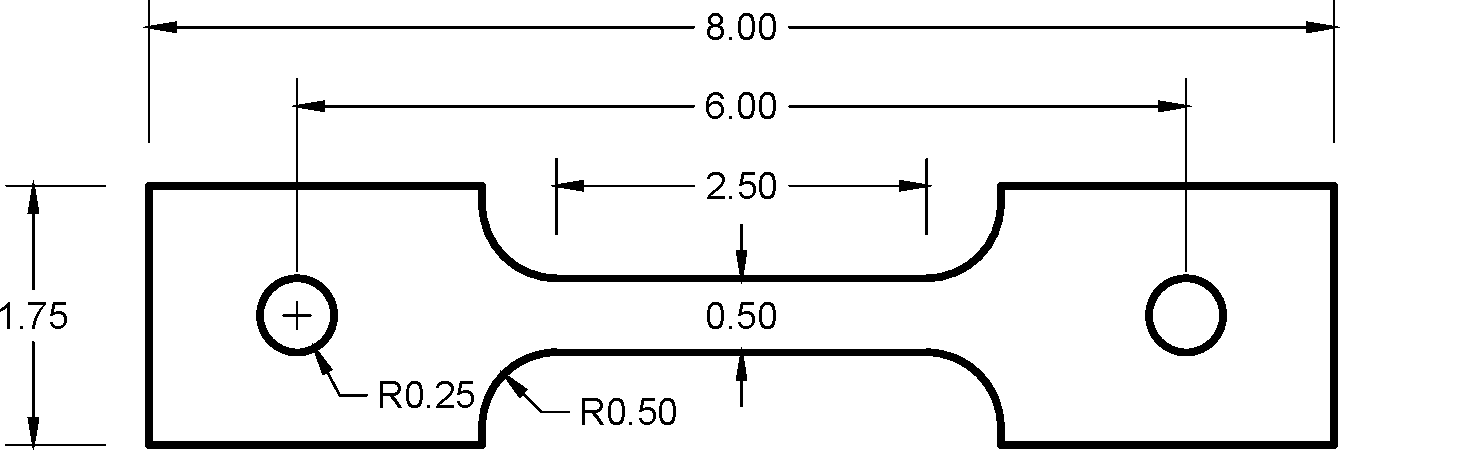
\includegraphics[width=6.0in]{figures/tensile_specimen_dimensions.pdf}
  \caption{Tensile specimen dimensions, in inches. The thickness of the plate specimen shown is $0.5$ in., resulting in a square cross-section along the gage length. The area shown in grey represents the eighth-symmetric modeling domain.}
  \label{fig:tensile_specimen_dimensions}
\end{figure}

The tests were simulated under quasi-static loading conditions. The (reflected) eighth-symmetric meshes shown in Figures \ref{fig:necking_hex_mesh} and \ref{fig:necking_poly_mesh} were used in conjunction with the FEM and DG-PEM, respectively. Both meshes consisted of roughly 400 elements. To assist with the initiation of necking, each mesh also contained a small geometric defect mid-way along the gage length: a 1\% reduction in the cross-sectional area of the specimen.

\begin{figure}[!h]
  \centering
    \begin{subfigure}[b]{0.49\linewidth}
            \centering
            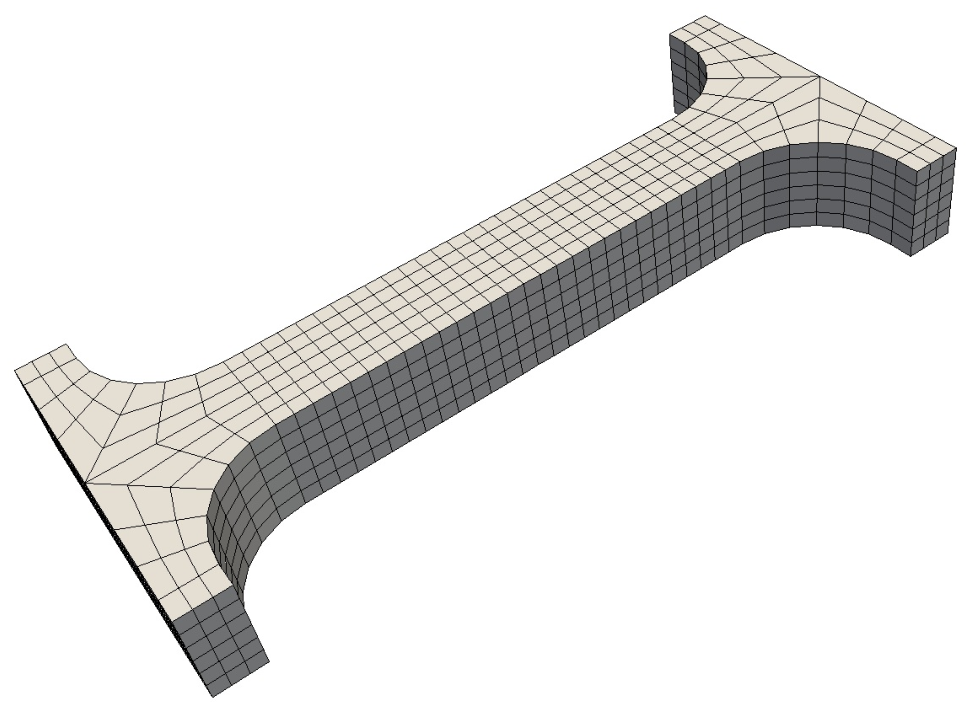
\includegraphics[width=3.0in]{figures/neck_hex_mesh.pdf}
    			\caption{Hexahedral mesh \label{fig:necking_hex_mesh}}
    \end{subfigure}
	\begin{subfigure}[b]{0.49\linewidth}
            \centering
            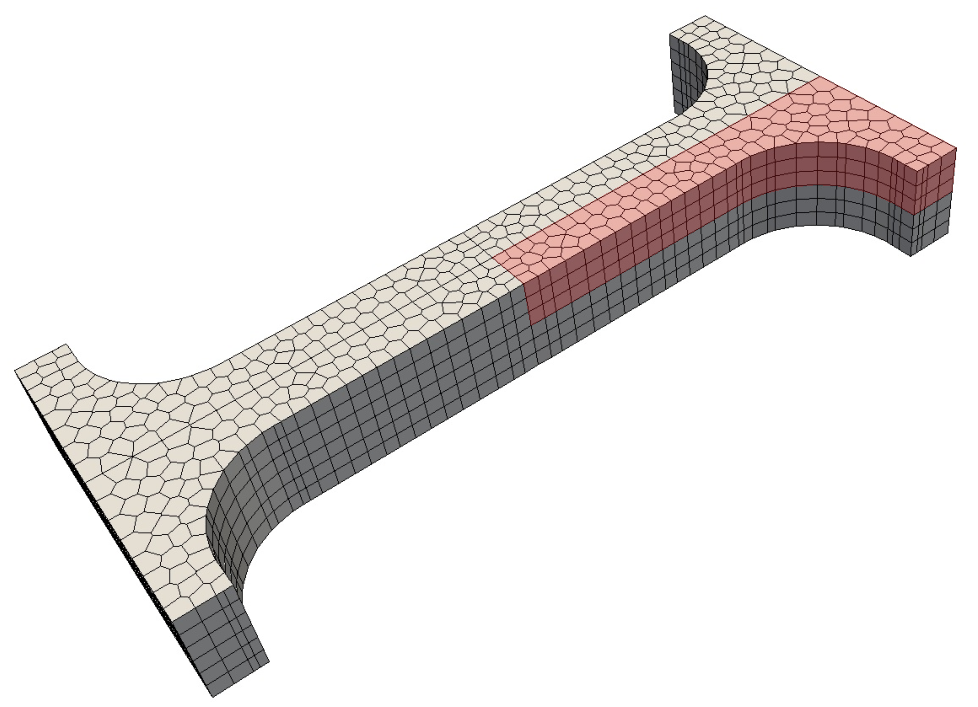
\includegraphics[width=3.0in]{figures/neck_poly_mesh.pdf}
    			\caption{Polyhedral mesh \label{fig:necking_poly_mesh}}
    \end{subfigure} \caption{Plate specimen meshes used for the tensile necking problem, modeled as an eighth-symmetric problem.}
  \label{fig:necking_meshes}
\end{figure}

Values of true (Cauchy) stress and engineering strain were measured from the analysis results via the post-processing tools available in ParaView \cite{ParaView}. The vertical component of Cauchy stress was averaged over the necked area of the specimen to determine an average tensile stress. To maintain consistency with the experimental procedures in \cite{Gerberich:62}, the engineering strain and percent elongation of the specimen were measured over a gage length of 2 inches. The \% reduction in area of the specimen was also recorded at the location of necking.

% listed in Table \ref{tab:tensile_specimen_properties}.
%\begin{table}[!ht]
%  \begin{center}
%    \begin{tabular}{| c || c | c |}
%    \hline
%      & 4130 steel (800$^{\circ}$F temper) & 4130 steel (1050$^{\circ}$F temper) \\ \hline \hline
%    $E$ (ksi) & 28000 & 28600 \\ \hline
%    	$\nu$ (in/in) & 0.29 & 0.29 \\ \hline
%    $Y_0$ (ksi) & 173 & 129 \\ \hline
%    $E_h$ (ksi) & 741 & 500 \\
%    \hline
%    \end{tabular}
%    \caption{Tensile specimen properties.}
%    \vspace{-5pt}
%    \label{tab:tensile_specimen_properties}
%    \vspace{-25pt}
%  \end{center}
%\end{table}

The visualized results of the simulations are depicted in Figure \ref{fig:necking_comparison}. When the kinematic enhancement is utilized, the results obtained using the FEM and the DG-PEM are comparable to one another. Both formulations succumb to volumetric locking if the enhancement is omitted. However, the polyhedral discretization used with the DG-PEM is less sensitive to the effects of locking, consistent with previous observations.

\begin{figure}[!h]
  \centering
    \begin{subfigure}[b]{1.0\linewidth}
            \centering
            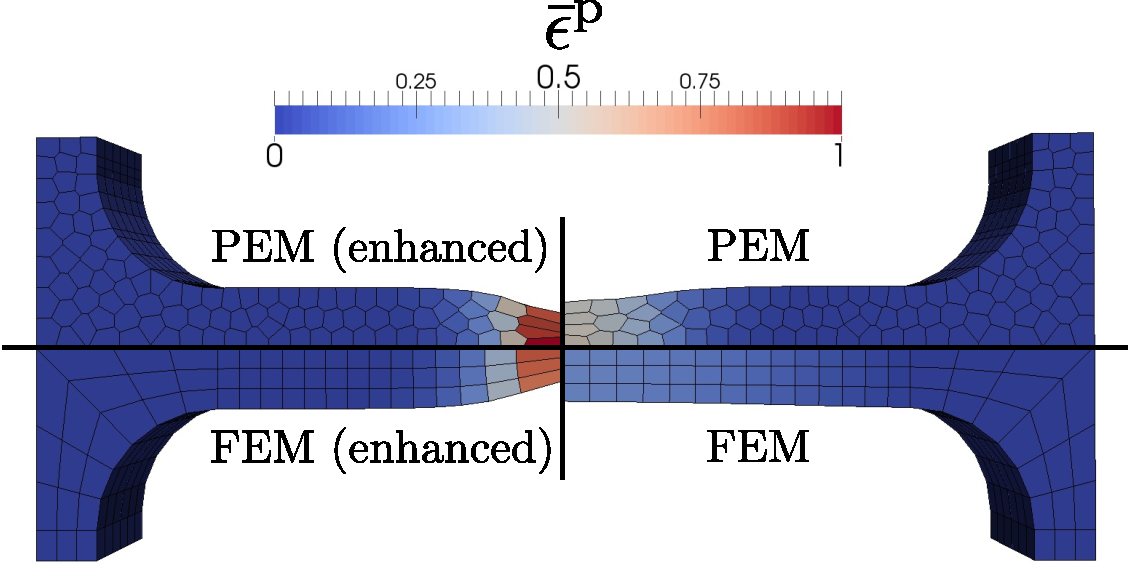
\includegraphics[width=6.0in]{figures/necking_comparison.pdf}
    			\caption{equivalent plastic strain $\bar{\epsilon}^p$ \label{fig:necking_eqps}}
    \end{subfigure}
	\begin{subfigure}[b]{1.0\linewidth}
            \centering
            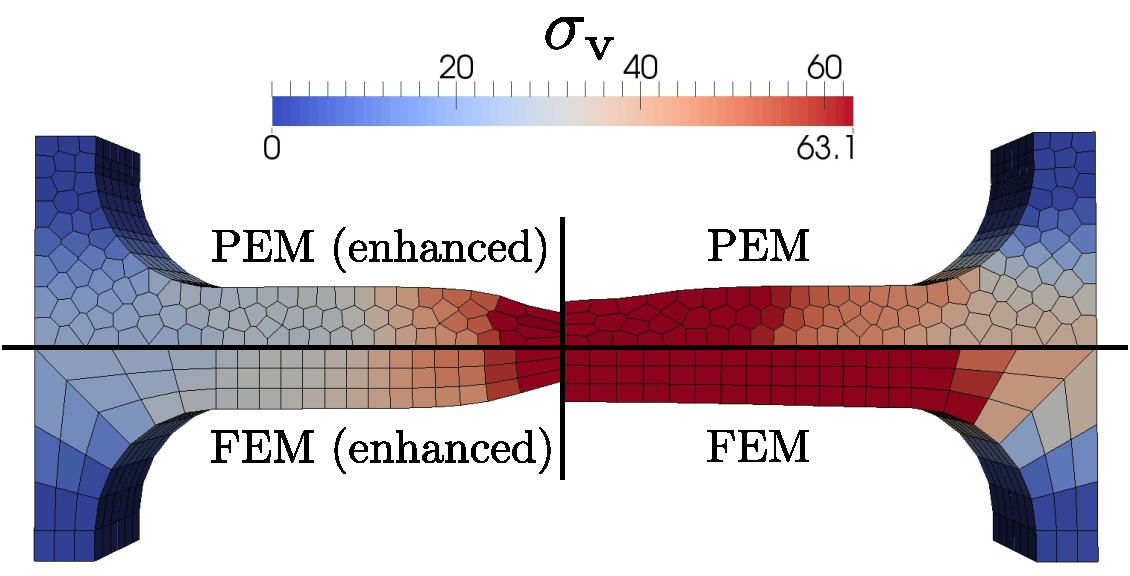
\includegraphics[width=6.0in]{figures/necking_vonMises.pdf}
    			\caption{von Mises stress $\sigma_v$ (ksi) \label{fig:necking_vonMises}}
    \end{subfigure} \caption{Comparison of necking behavior at 16.5\% elongation, depicting deformed shapes and color map values of equivalent plastic strain $\bar{\epsilon}^p$ and von Mises stress $\sigma_v$ (ksi).}
  \label{fig:necking_comparison}
\end{figure}

Plots of the computed (Cauchy) stress vs. engineering strain curves from each simulation are depicted in Figure \ref{fig:necking_stress_strain}. Additionally, Figure \ref{fig:necking_area_reduction} compares the decrease in the necked area of the specimen vs. engineering strain. In each plot, the results for the FEM and the DG-PEM provide comparable accuracy if the kinematic enhancement is employed. If the enhancement is not utilized, the FEM performs more poorly than the DG-PEM, exhibiting little to no necking behavior.

\begin{figure}[!h]
  \centering
    \begin{subfigure}[b]{0.49\linewidth}
            \centering
            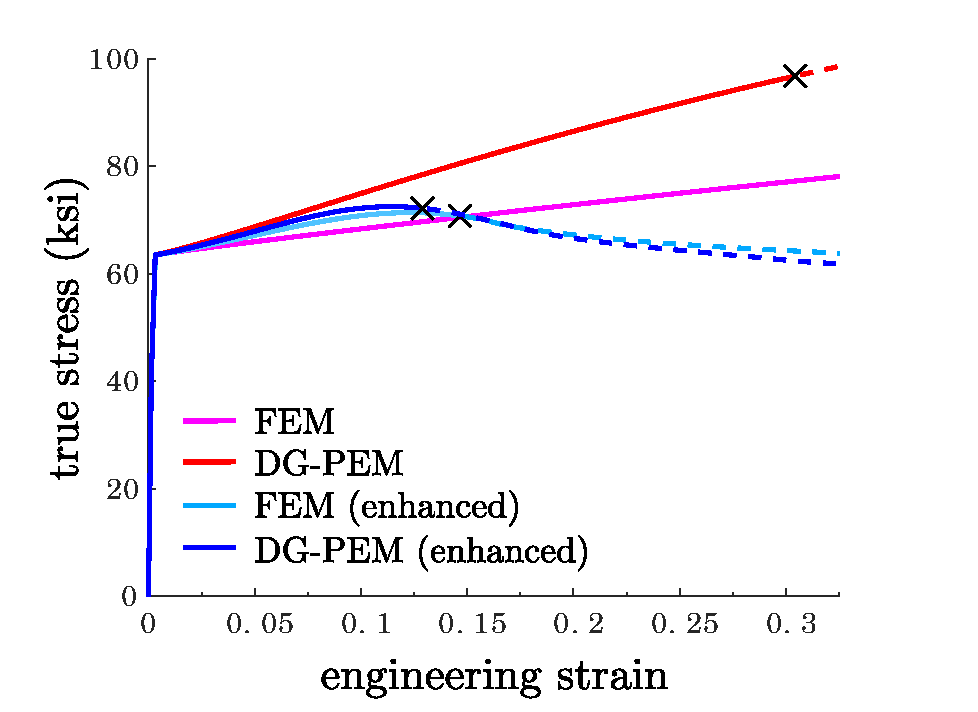
\includegraphics[width=3.5in]{figures/necking_stress_strain.pdf}
    			\caption{True stress vs. engineering strain \label{fig:necking_stress_strain}}
    \end{subfigure}
	\begin{subfigure}[b]{0.49\linewidth}
            \centering
            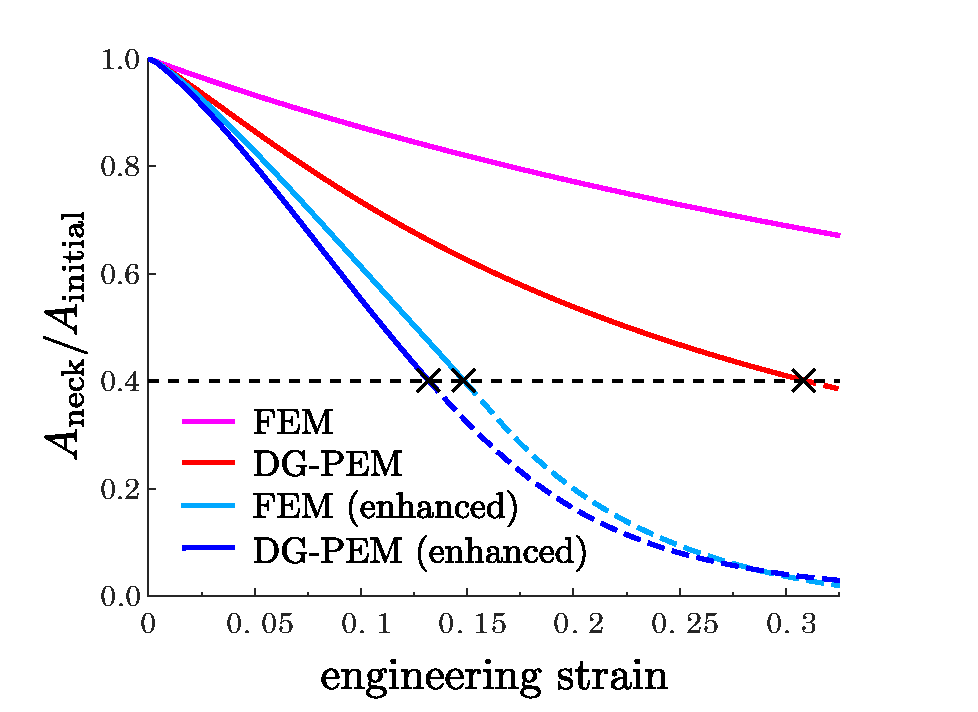
\includegraphics[width=3.5in]{figures/necking_area_reduction.pdf}
    			\caption{Reduced area vs. engineering strain \label{fig:necking_area_reduction}}
    \end{subfigure} \caption{Plotted results for the FEM and DG-PEM models, both with and without the kinematic enhancement discussed in \cite{Rashid:06}. The estimated point of rupture is indicated by an X in each plot.}
  \label{fig:necking_plots}
\end{figure}

%\begin{figure}[!h]
%    \centering
%    \begin{subfigure}[b]{0.49\linewidth}
%            \centering
%            \includegraphics[width=3.0in]{figures/necking_eqps_0.pdf}
%    			\caption{$t=0.0$ \label{fig:necking_eqps_0}}
%    \end{subfigure}
%	\begin{subfigure}[b]{0.49\linewidth}
%            \centering
%            \includegraphics[width=3.0in]{figures/necking_eqps_1.pdf}
%    			\caption{$t=0.5$ \label{fig:necking_eqps_1}}
%    \end{subfigure}
%    \begin{subfigure}[b]{0.49\linewidth}
%            \centering
%            \includegraphics[width=3.0in]{figures/necking_eqps_2.pdf}
%    			\caption{$t=0.75$ \label{fig:necking_eqps_2}}
%    \end{subfigure}
%	\begin{subfigure}[b]{0.49\linewidth}
%            \centering
%            \includegraphics[width=3.0in]{figures/necking_eqps_3.pdf}
%    			\caption{$t=1$ \label{fig:necking_eqps_3}}
%    \end{subfigure}
%    \caption{Comparison of necking behavior at various times during the analysis, depicting deformed shape, and values of equivalent plastic strain.}
%    \label{fig:necking_eqps}
%\end{figure}

%\begin{table}
%\centering
%\begin{subtable}{1.0\textwidth}
%\centering
%\begin{tabular}{| c || c | c | c |}
%    \hline
%               & \% elongation (2 in) & \% area reduction & UTS (ksi) \\ \hline \hline
%    FEM        &  &  &  \\ \hline
%    DG-PEM     &  &  &  \\ \hline
%    Experiment & 6 & 36.7 & 182 \\
%    \hline
%    \end{tabular}
%    \caption{4130 steel (800$^\circ$F temper)}
%    \label{tab:tensile_test_data_results800}
%\end{subtable}% <---- don't forget this %
%\\
%\begin{subtable}{1.0\textwidth}
%\centering
%\begin{tabular}{| c || c | c | c |}
%    \hline
%               & \% elongation (2 in) & \% area reduction & UTS (ksi) \\ \hline \hline
%    FEM        &  &  &  \\ \hline
%    DG-PEM     &  &  &  \\ \hline
%    Experiment & 10 & 49.7 & 136 \\
%    \hline
%    \end{tabular}
%    \caption{4130 steel (1050$^\circ$F temper)}
%    \label{tab:tensile_test_data_results1050}
%\end{subtable}
%\caption{Tensile test data results comparison.}
%\label{tab:tensile_test_data_results}
%\end{table}

Without the use of an adequate model for ductile fracture, it is not possible to predict when rupture will occur within the specimen. Nonetheless, an ad hoc metric of 60\% reduction in area is used herein to \textit{estimate} the point of rupture, with the \% elongation at failure recorded at this point in the analysis. Table \ref{tab:tensile_test_data_results} shows the recorded values of \% elongation at failure and maximum tensile stress for the FEM and DG-PEM simulations. These results were compared against a more refined solution obtained using the FEM, showing that the DG-PEM performs comparatively well on the polyhedral mesh at coarser levels of refinement.

\begin{table}
\centering
\begin{tabular}{| l || c | c |}
    \hline
               & \% elongation at failure & max tensile stress (ksi) \\ \hline \hline
    FEM (enhanced)    & 14.65 & 70.74 \\ \hline
    DG-PEM (enhanced) & 12.89 & 72.15 \\ \hline
    FEM (refined)     & 13.35 & 75.58 \\
    \hline
\end{tabular}
\caption{Tensile test data results comparison. The values of \% elongation were recorded after reaching 60\% reduction in area.}
\label{tab:tensile_test_data_results}
\end{table}

If the PEM is employed on the hexahedral mesh in Figure \ref{fig:necking_hex_mesh}, the results are comparable with those of the FEM. As noted in the twisting annulus problem, this suggests that arbitrary polyhedral discretizations may be less sensitive to the effects of volumetric locking. The consequences of this decreased sensitivity are further explored in the subsequent problem.

\subsection*{Taylor Bar Impact Problem}

A standard problem in the literature entailing high plastic flow is the Taylor bar impact test. For the present study, an impact test for an OFHC copper rod will be investigated. The HTT-$\alpha$ implicit dynamics time integration algorithm \cite{Hilber&Hughes&Taylor:77} is utilized with $\alpha = -0.1$.

For high impact velocities, the Taylor impact test is canonically modeled as a coupled thermo-mechanical problem. Moreover, many finite element simulations (\cite{Heinstein:05}, \cite{Banerjee:05}) employ temperature- and strain-rate-dependent material models (such as the model of Johnson and Cook \cite{Johnson&Cook:83}). To avoid over-complicating the subsequent analyses, however, isothermal conditions are assumed. Additionally, the simple (rate-independent) $J_2$ elasto-plasticity model described previously will be utilized. The following model parameters were taken from \cite{Erhart:11}: $E = 117$ GPa, $\nu = 0.35$, $Y_0 = 0.4$ GPa, $E_h = 0.1$ GPa, and $\rho_0=$ 8,930 kg/$\text{m}^3$.

The experimental procedures detailed in \cite{Johnson&Cook:83} and \cite{Gust:82} are emulated. As in \cite{Johnson&Cook:83}, the impact specimen was a cylindrical copper rod with an initial height of 30 mm, and an initial diameter of 6 mm. Prior to impact, the rod was given an initial velocity of $200$ m/s.

Frictionless contact between the rod and a rigid surface corresponding to $X_3 = 0.0$ was modeled via the inclusion of a penalty traction of the form:
\begin{equation}
	\bar{t}_1 = \bar{t}_2 = 0, \quad \bar{t}_3 = p \langle -u_3|u_3|  \rangle.
	\label{eq:penalty_traction}
\end{equation}
In (\ref{eq:penalty_traction}), $u_3$ corresponds to the vertical displacement of a given point on the bottom face of the rod, $\langle \cdot \rangle$ denote the Macaulay brackets, and $p$ is a penalty stiffness parameter. For the problem at hand, an ad hoc value of $p = 6.0 \times 10^{10} \, \text{GPa}/\text{mm}^2$ was chosen (following a process of trial-and-error).

The (reflected) quarter-symmetric meshes shown in Figures \ref{fig:taylor_bar_hex_mesh} and \ref{fig:taylor_bar_poly_mesh} were used in conjunction with the FEM and DG-PEM, respectively. Both meshes consisted of roughly 1000 elements, each.

\begin{figure}[!h]
  \centering
    \begin{subfigure}[b]{0.49\linewidth}
            \centering
            \includegraphics[width=3.0in]{figures/taylor_bar_hex_mesh.pdf}
    			\caption{Hexahedral mesh \label{fig:taylor_bar_hex_mesh}}
    \end{subfigure}
	\begin{subfigure}[b]{0.49\linewidth}
            \centering
            \includegraphics[width=3.0in]{figures/taylor_bar_poly_mesh.pdf}
    			\caption{Prismatic polyhedral mesh \label{fig:taylor_bar_poly_mesh}}
    \end{subfigure} \caption{Impact specimen meshes used for the Taylor bar problem, modeled using quarter-symmetry.}
  \label{fig:taylor_bar_meshes}
\end{figure}

Because high plastic flow is expected, volumetric locking is a concern. Once again, the kinematic enhancement of \cite{Rashid:06} is employed to address this issue. However, an interesting result occurs for the Taylor impact problem if the kinematic enhancement is applied to the polyhedral mesh in Figure \ref{fig:taylor_bar_poly_mesh}. Specifically, the polyhedral mesh becomes tangled, as illustrated in Figure \ref{fig:element_inversion}. The elements become overly flexible with respect to the isochoric modes of deformation, and inertial effects are sufficient to cause the elements to ultimately invert after just a few time steps. For this reason, a complete analysis could not be run for the DG-PEM using the kinematic enhancement.

\begin{figure}[!h]
  \centering
    \begin{subfigure}[b]{0.49\linewidth}
            \centering
            \includegraphics[width=2.0in]{figures/before_distortion.pdf}
    			\caption{$t = 0.0$ ms \label{fig:before_distortion}}
    \end{subfigure}
	\begin{subfigure}[b]{0.49\linewidth}
            \centering
            \includegraphics[width=2.0in]{figures/after_distortion.pdf}
    			\caption{$t = 0.002$ ms \label{fig:after_distortion}}
    \end{subfigure} \caption{DG-PEM element inversion when using the kinematic enhancement of \cite{Rashid:06}, viewed from the bottom of the mesh (the impacting surface).}
  \label{fig:element_inversion}
\end{figure}

Figures \ref{fig:taylor_bar_eqps} and \ref{fig:taylor_bar_stresses} provide illustrations of the results of each simulation. Without the kinematic enhancement, the hexahedral FEM mesh clearly suffers from volumetric locking. Interestingly, the polyhedral DG-PEM mesh does not appear to exhibit any serious symptoms of volumetric locking, yielding comparable results to the kinematically enhanced FEM solution.

\begin{figure}[!h]
    \centering
    \begin{subfigure}[b]{0.49\linewidth}
            \centering
            \includegraphics[width=3.0in]{figures/taylor_bar_unmodified_eqps.pdf}
    			\caption{FEM vs. PEM \label{fig:taylor_bar_unmodified_eqps}}
    \end{subfigure}
	\begin{subfigure}[b]{0.49\linewidth}
            \centering
            \includegraphics[width=3.0in]{figures/taylor_bar_fbar_eqps.pdf}
    			\caption{(enhanced) FEM vs. (unenhanced) PEM \label{fig:taylor_bar_fbar_eqps}}
    \end{subfigure}
    \caption{Comparison of results between the FEM and PEM models at the final time $t = 0.08$ ms, depicting deformed shape and color map values of equivalent plastic strain $\bar{\epsilon}^p$.}
    \label{fig:taylor_bar_eqps}
\end{figure}

\begin{figure}[!h]
  \centering
    \begin{subfigure}[b]{0.32\linewidth}
            \centering
            \includegraphics[width=2.1in]{figures/taylor_bar_fem_unmodified.pdf}
    			\caption{FEM \label{fig:taylor_bar_fem_unmodified}}
    \end{subfigure}
	\begin{subfigure}[b]{0.32\linewidth}
            \centering
            \includegraphics[width=2.1in]{figures/taylor_bar_pem_unmodified.pdf}
    			\caption{DG-PEM \label{fig:taylor_bar_pem_unmodified}}
    \end{subfigure} 
    \begin{subfigure}[b]{0.32\linewidth}
            \centering
            \includegraphics[width=2.1in]{figures/taylor_bar_fem_fbar.pdf}
    			\caption{FEM (enhanced) \label{fig:taylor_bar_fem_fbar}}
    \end{subfigure} 
    \caption{Comparison of von Mises stress $\sigma_v$ (in Pascals) within the FEM and PEM models at the final time $t = 0.08$ ms.}
  \label{fig:taylor_bar_stresses}
\end{figure}

To provide a more quantitative comparison of the results obtained for each method, two canonical deformation metrics are considered: the rod's final base diameter $D_{\text{final}}$ and compressed length $L_{\text{final}}$, measured after the rod has achieved full impact. The results are displayed in Table \ref{tab:change_in_length_measurements}, and compared against a more refined solution obtained using the FEM. Despite the apparent stability issues pertaining to the kinematic enhancement, the data indicate that the DG-PEM performs favorably in comparison with the FEM.

\begin{table}[!ht]
  \begin{center}
    \begin{tabular}{| l || c | c |}
    \hline
                & $D_{\text{final}}$ (mm) & $L_{\text{final}}$ (mm) \\ \hline \hline
    FEM               & 11.37 & 23.04 \\ \hline
    DG-PEM            & 13.47 & 23.38 \\ \hline
    FEM (enhanced)    & 13.91 & 23.60 \\ \hline
    DG-PEM (enhanced) & (unstable) & (unstable) \\ \hline
    FEM (refined)     & 13.87 & 23.61 \\
    \hline
    \end{tabular}
    \caption{Measurements of the rod's final base diameter $D_{\text{final}}$ and overall length $L_{\text{final}}$.}
    \vspace{-5pt}
    \label{tab:change_in_length_measurements}
    \vspace{-10pt}
  \end{center}
\end{table}

The issue of element inversion when using arbitrary polyhedral discretizations for highly dynamic problems warrants further investigation. Evidently, the kinematic enhancement of \cite{Rashid:06} is not adequate for general element shapes. Because arbitrary polyhedra possess more nodes (degrees of freedom) than traditional hexahedra, a ``mean'' dilatation formulation is likely to result in under-constrained modes of deformation. A more intricate, and element-specific enhancement is needed. This issue is left as the subject of future work.